\documentclass[11pt,a4paper]{article}
\usepackage[utf8]{inputenc}
\usepackage[margin=0.8in]{geometry}
\setlength{\headheight}{14pt}
\usepackage{graphicx}
\usepackage{amsmath,amssymb}
\usepackage{booktabs}
\usepackage{longtable}
\usepackage{array}
\usepackage{hyperref}
\usepackage{float}
\usepackage{caption}
\usepackage{subcaption}
\usepackage{fancyhdr}
\usepackage{titlesec}
\usepackage{xcolor}

% Custom Colors
\definecolor{primary}{RGB}{0, 51, 102}
\definecolor{secondary}{RGB}{70, 130, 180}

\hypersetup{
    colorlinks=true,
    linkcolor=primary,
    citecolor=primary,
    urlcolor=secondary
}

% Header and Footer setup
\pagestyle{fancy}
\fancyhf{}
\rhead{\textcolor{primary}{\textbf{EDC Laboratory --- Experiment 2}}}
\lhead{\textcolor{primary}{\textbf{EE25BTECH11056 \& EE25BTECH11049}}}
\rfoot{Page \thepage}

\titleformat{\section}{\large\bfseries\color{primary}}{\thesection.}{0.5em}{}
\titleformat{\subsection}{\normalfont\bfseries\color{secondary}}{\thesubsection}{0.5em}{}
\titleformat{\subsubsection}{\normalfont\bfseries}{\thesubsubsection}{0.5em}{}

\begin{document}

% Title Page / Header Block
\begin{center}
    {\LARGE \textbf{\color{primary} DEPARTMENT OF ELECTRICAL ENGINEERING}}\\[0.2cm]
    {\large \textbf{Electronic Devices \& Circuits Laboratory (EDC LAB)}}\\[0.4cm]
    \rule{\linewidth}{1pt}\\[0.3cm]
    {\Large \textbf{EXPERIMENT 2: Input \& Output Characteristics of BJT in Common Emitter (CE), Common Base (CB), and Common Collector (CC) Configurations}}\\[0.3cm]
    \rule{\linewidth}{1pt}\\[0.4cm]
    
    \begin{tabular}{ll}
      \textbf{Prepared By:} & \textbf{Suraj.N (EE25BTECH11056)} \\
                            & \textbf{Sai Krishna Bakki (EE25BTECH11049)} \\
        \textbf{Course:} & Electronic Devices \& Circuits Lab \\
        \textbf{Date:} & \today
    \end{tabular}
\end{center}

\vspace{0.3cm}

\section{Aim}
\begin{enumerate}
    \item To study and plot the input and output characteristics of a BJT (BC547 NPN Transistor) in the \textbf{Common Emitter (CE)} configuration, and to determine the common-emitter current gain ($\beta$), input resistance ($r_i$), and output resistance ($r_o$).
    \item To study and plot the input and output characteristics of a BJT in the \textbf{Common Base (CB)} configuration, and to determine the common-base current gain ($\alpha$), input resistance ($r_i$), and output resistance ($r_o$).
    \item To study and plot the input and output characteristics of a BJT in the \textbf{Common Collector (CC)} configuration, and to determine the common-collector current gain ($\gamma$), input resistance ($r_i$), and output resistance ($r_o$).
    \item To verify the mathematical relationships between current gains: $\beta = \frac{\alpha}{1-\alpha}$ and $\gamma = \beta + 1$ using measured parameters.
\end{enumerate}

\section{Apparatus and Software Tools Required}
\begin{table}[H]
\centering
\caption{Equipment, Components, and Software Specifications}
\begin{tabular}{cllc}
\toprule
\textbf{S.No.} & \textbf{Component / Equipment} & \textbf{Specification} & \textbf{Quantity} \\
\midrule
1 & NPN Transistor & BC547 (TO-92 package) & 1 \\
2 & Resistors & $1\text{ k}\Omega$, $10\text{ k}\Omega$ & 1 each \\
3 & Regulated DC Power Supplies & Variable $0\text{--}30\text{ V}$ Dual Output & 2 \\
4 & Digital Ammeters / Microammeters & $0\text{--}500\ \mu\text{A}$, $0\text{--}10\text{ mA}$ & As required \\
5 & Digital Voltmeters & $0\text{--}1\text{ V}$, $0\text{--}30\text{ V}$ & As required \\
6 & Simulation Software & LTspice XVII & -- \\
\bottomrule
\end{tabular}
\end{table}

\section{Overall Theoretical Background}
A Bipolar Junction Transistor (BJT) is a three-terminal, current-controlled semiconductor device consisting of two PN junctions (emitter-base junction $J_{EB}$ and collector-base junction $J_{CB}$). The behavior of the transistor in any circuit configuration depends primarily on the biasing conditions of these two junctions:
\begin{itemize}
    \item \textbf{Cut-off Region:} Both $J_{EB}$ and $J_{CB}$ are reverse-biased. Transistor is OFF, $I_C \approx 0$.
    \item \textbf{Active Region:} $J_{EB}$ is forward-biased and $J_{CB}$ is reverse-biased. Transistor operates as an amplifier.
    \item \textbf{Saturation Region:} Both $J_{EB}$ and $J_{CB}$ are forward-biased. Transistor acts as a closed switch, $V_{CE} \approx V_{CE(\text{sat})}$.
\end{itemize}
Depending on which terminal is kept common to both input and output ports, BJTs are analyzed in three distinct configurations: Common Emitter (CE), Common Base (CB), and Common Collector (CC).

\clearpage

\section{Part A \& B: Common Emitter (CE) Configuration}

\subsection{Theoretical Background}
In the Common Emitter (CE) configuration, the emitter terminal is common to both the input (base-emitter) and output (collector-emitter) circuits. 
\begin{itemize}
    \item \textbf{Input Characteristics:} Plot of Base Current ($I_B$) vs Base-Emitter Voltage ($V_{BE}$) at constant Collector-Emitter Voltage ($V_{CE}$). It behaves like a forward-biased diode curve. As $V_{CE}$ increases, the effective base width decreases (Early effect / Base-width modulation), shifting the input curve slightly to the right.
    \item \textbf{Output Characteristics:} Plot of Collector Current ($I_C$) vs $V_{CE}$ at constant $I_B$. In the active region, $I_C = \beta I_B$, showing flat curves with high output resistance.
    \item \textbf{Key Parameters:}
    \begin{align}
        \text{Input Resistance: } r_i &= \left. \frac{\Delta V_{BE}}{\Delta I_B} \right|_{V_{CE} = \text{const}} \quad (\approx 1\text{ k}\Omega\text{ -- }5\text{ k}\Omega) \\
        \text{Output Resistance: } r_o &= \left. \frac{\Delta V_{CE}}{\Delta I_C} \right|_{I_B = \text{const}} \quad (\approx 50\text{ k}\Omega\text{ -- }100\text{ k}\Omega) \\
        \text{Current Gain: } \beta &= \left. \frac{\Delta I_C}{\Delta I_B} \right|_{V_{CE} = \text{const}} \quad (\approx 50\text{ -- }300)
    \end{align}
\end{itemize}

\subsection{Circuit Schematic and Simulation Waveforms}
\begin{figure}[H]
    \centering
    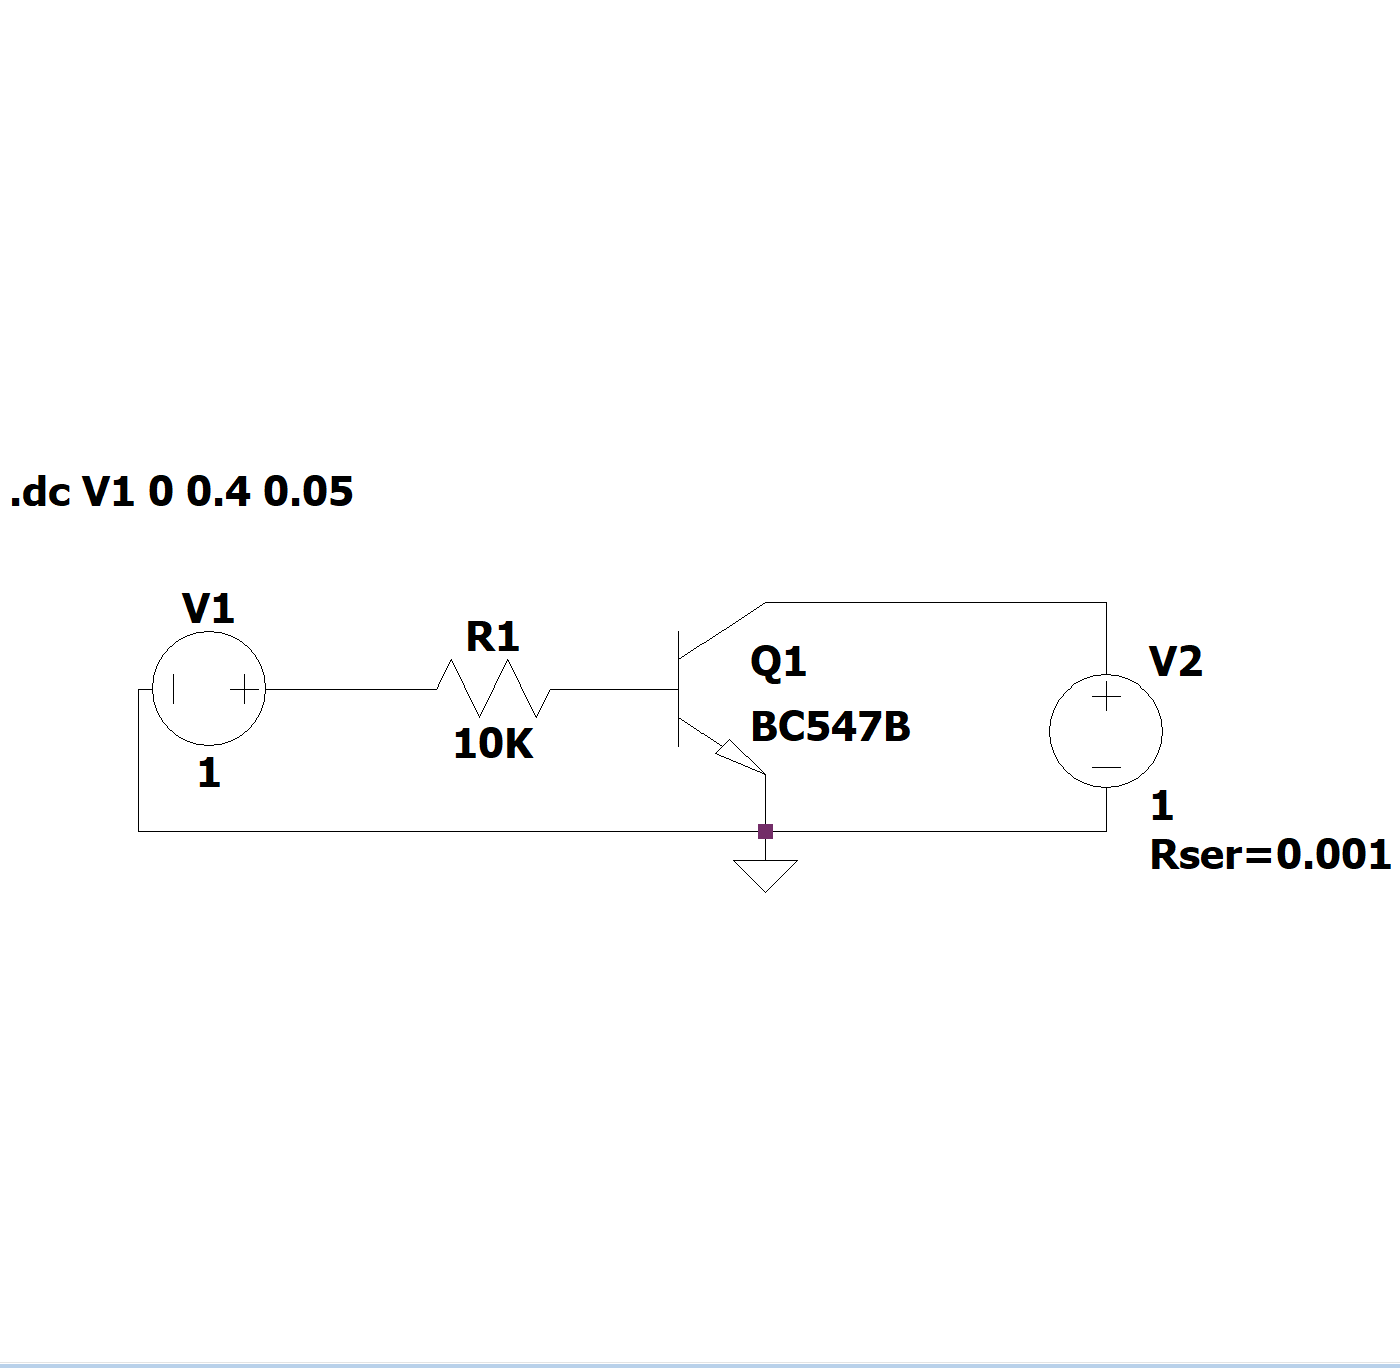
\includegraphics[width=0.55\textwidth]{../CE-Configuration/schematic.png}
    \caption{LTspice Circuit Schematic for Common Emitter (CE) Configuration.}
    \label{fig:ce_schematic}
\end{figure}

\subsubsection{CE Input Characteristics Simulation}
\begin{figure}[H]
    \centering
    \begin{subfigure}[b]{0.31\textwidth}
        \centering
        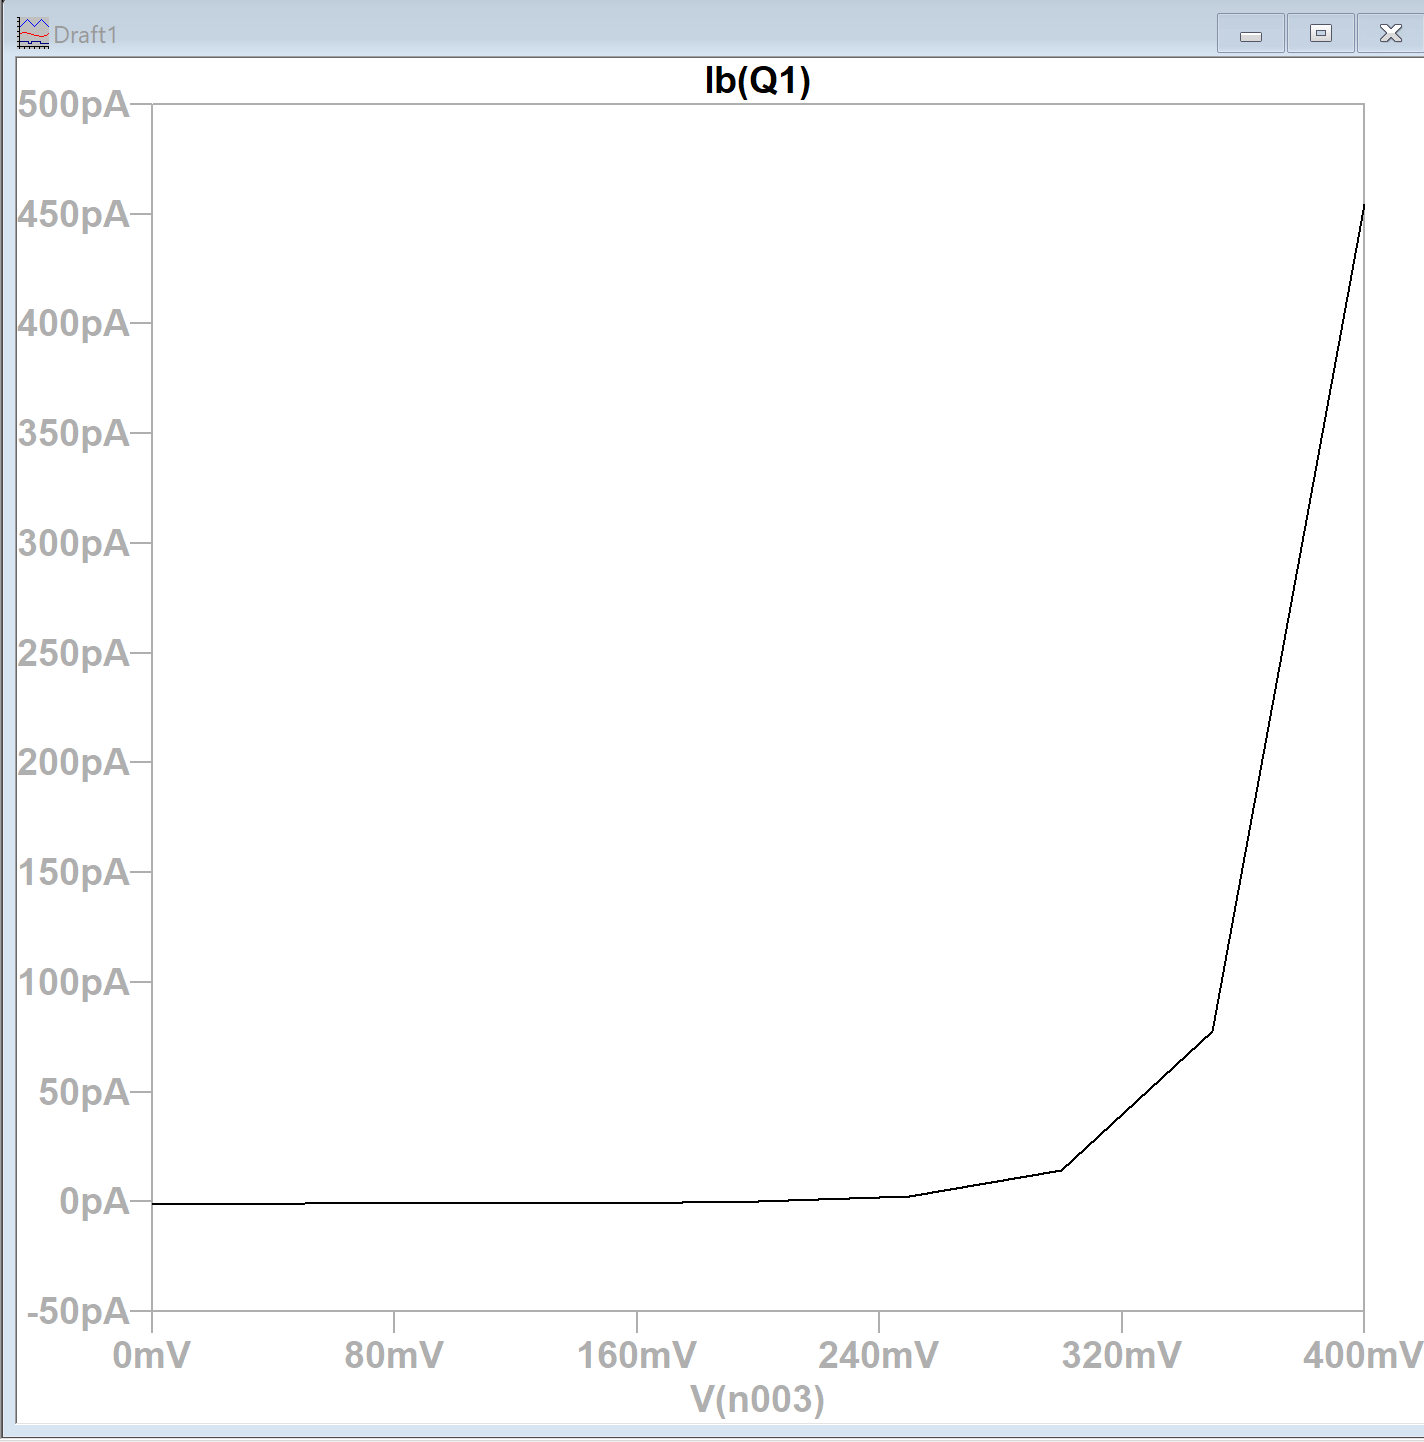
\includegraphics[width=\textwidth]{../CE-Configuration/input/input_0-0.4V_VCE=1.png}
        \caption{$0\text{--}0.4\text{ V}$ ($V_{CE} = 1\text{ V}$)}
    \end{subfigure}
    \hfill
    \begin{subfigure}[b]{0.31\textwidth}
        \centering
        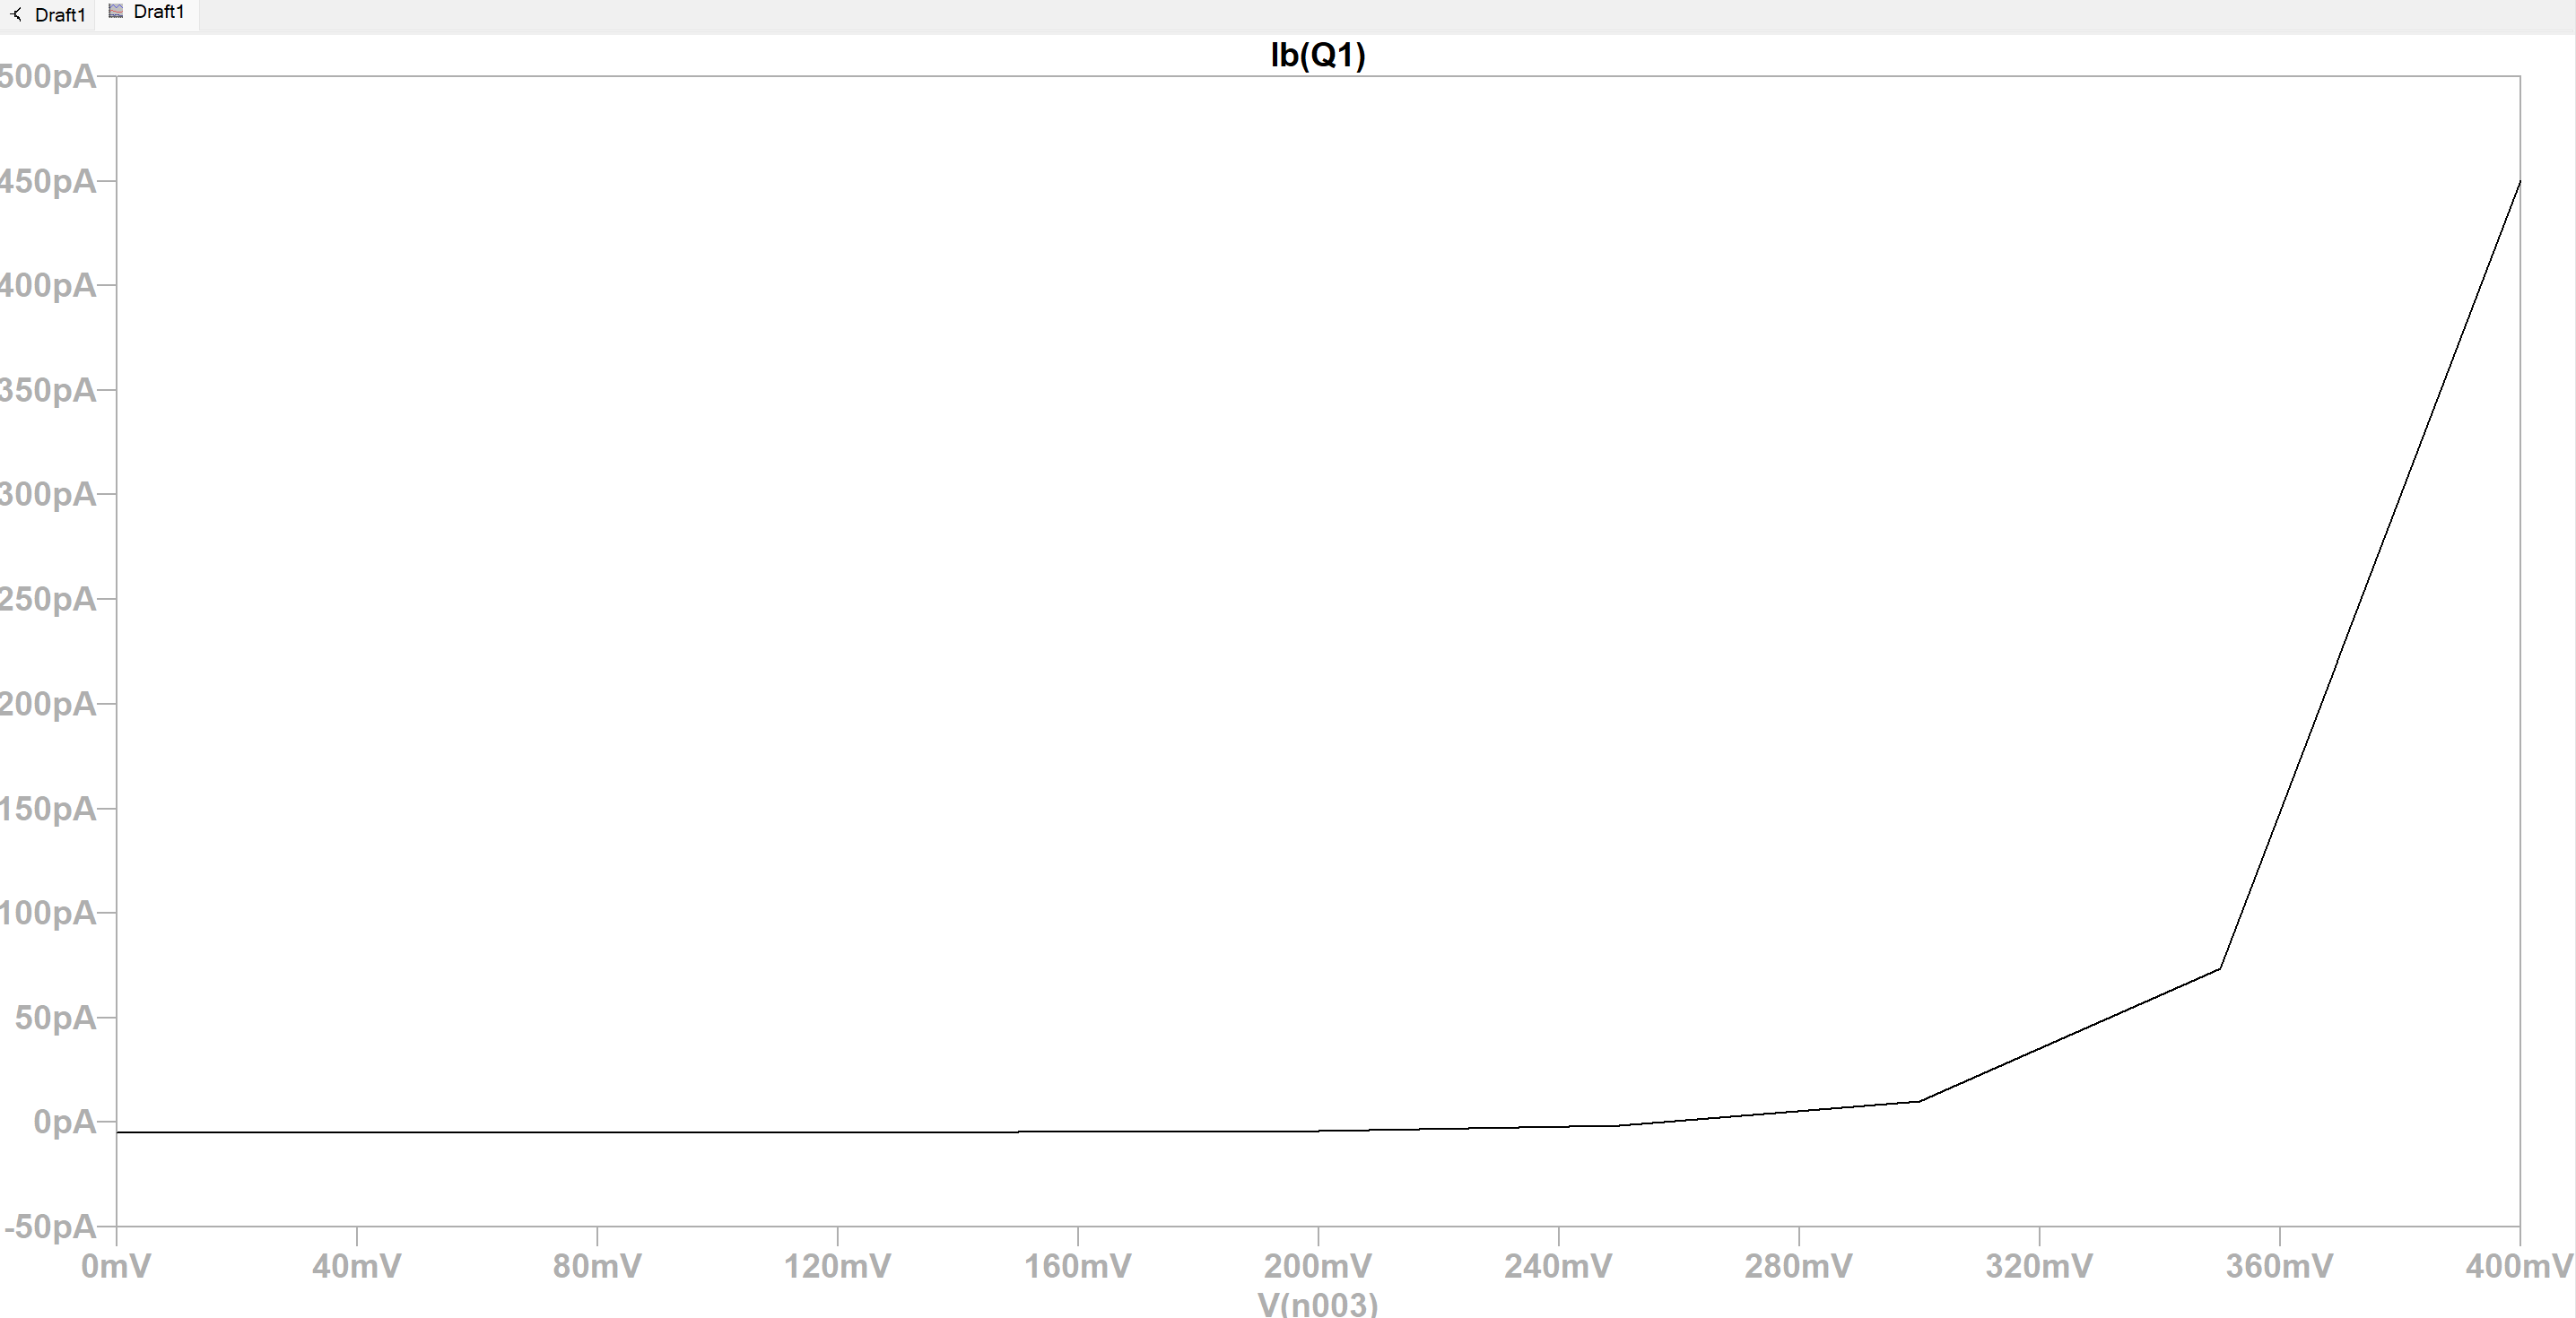
\includegraphics[width=\textwidth]{../CE-Configuration/input/input_0-0.4_VCE=5.png}
        \caption{$0\text{--}0.4\text{ V}$ ($V_{CE} = 5\text{ V}$)}
    \end{subfigure}
    \hfill
    \begin{subfigure}[b]{0.31\textwidth}
        \centering
        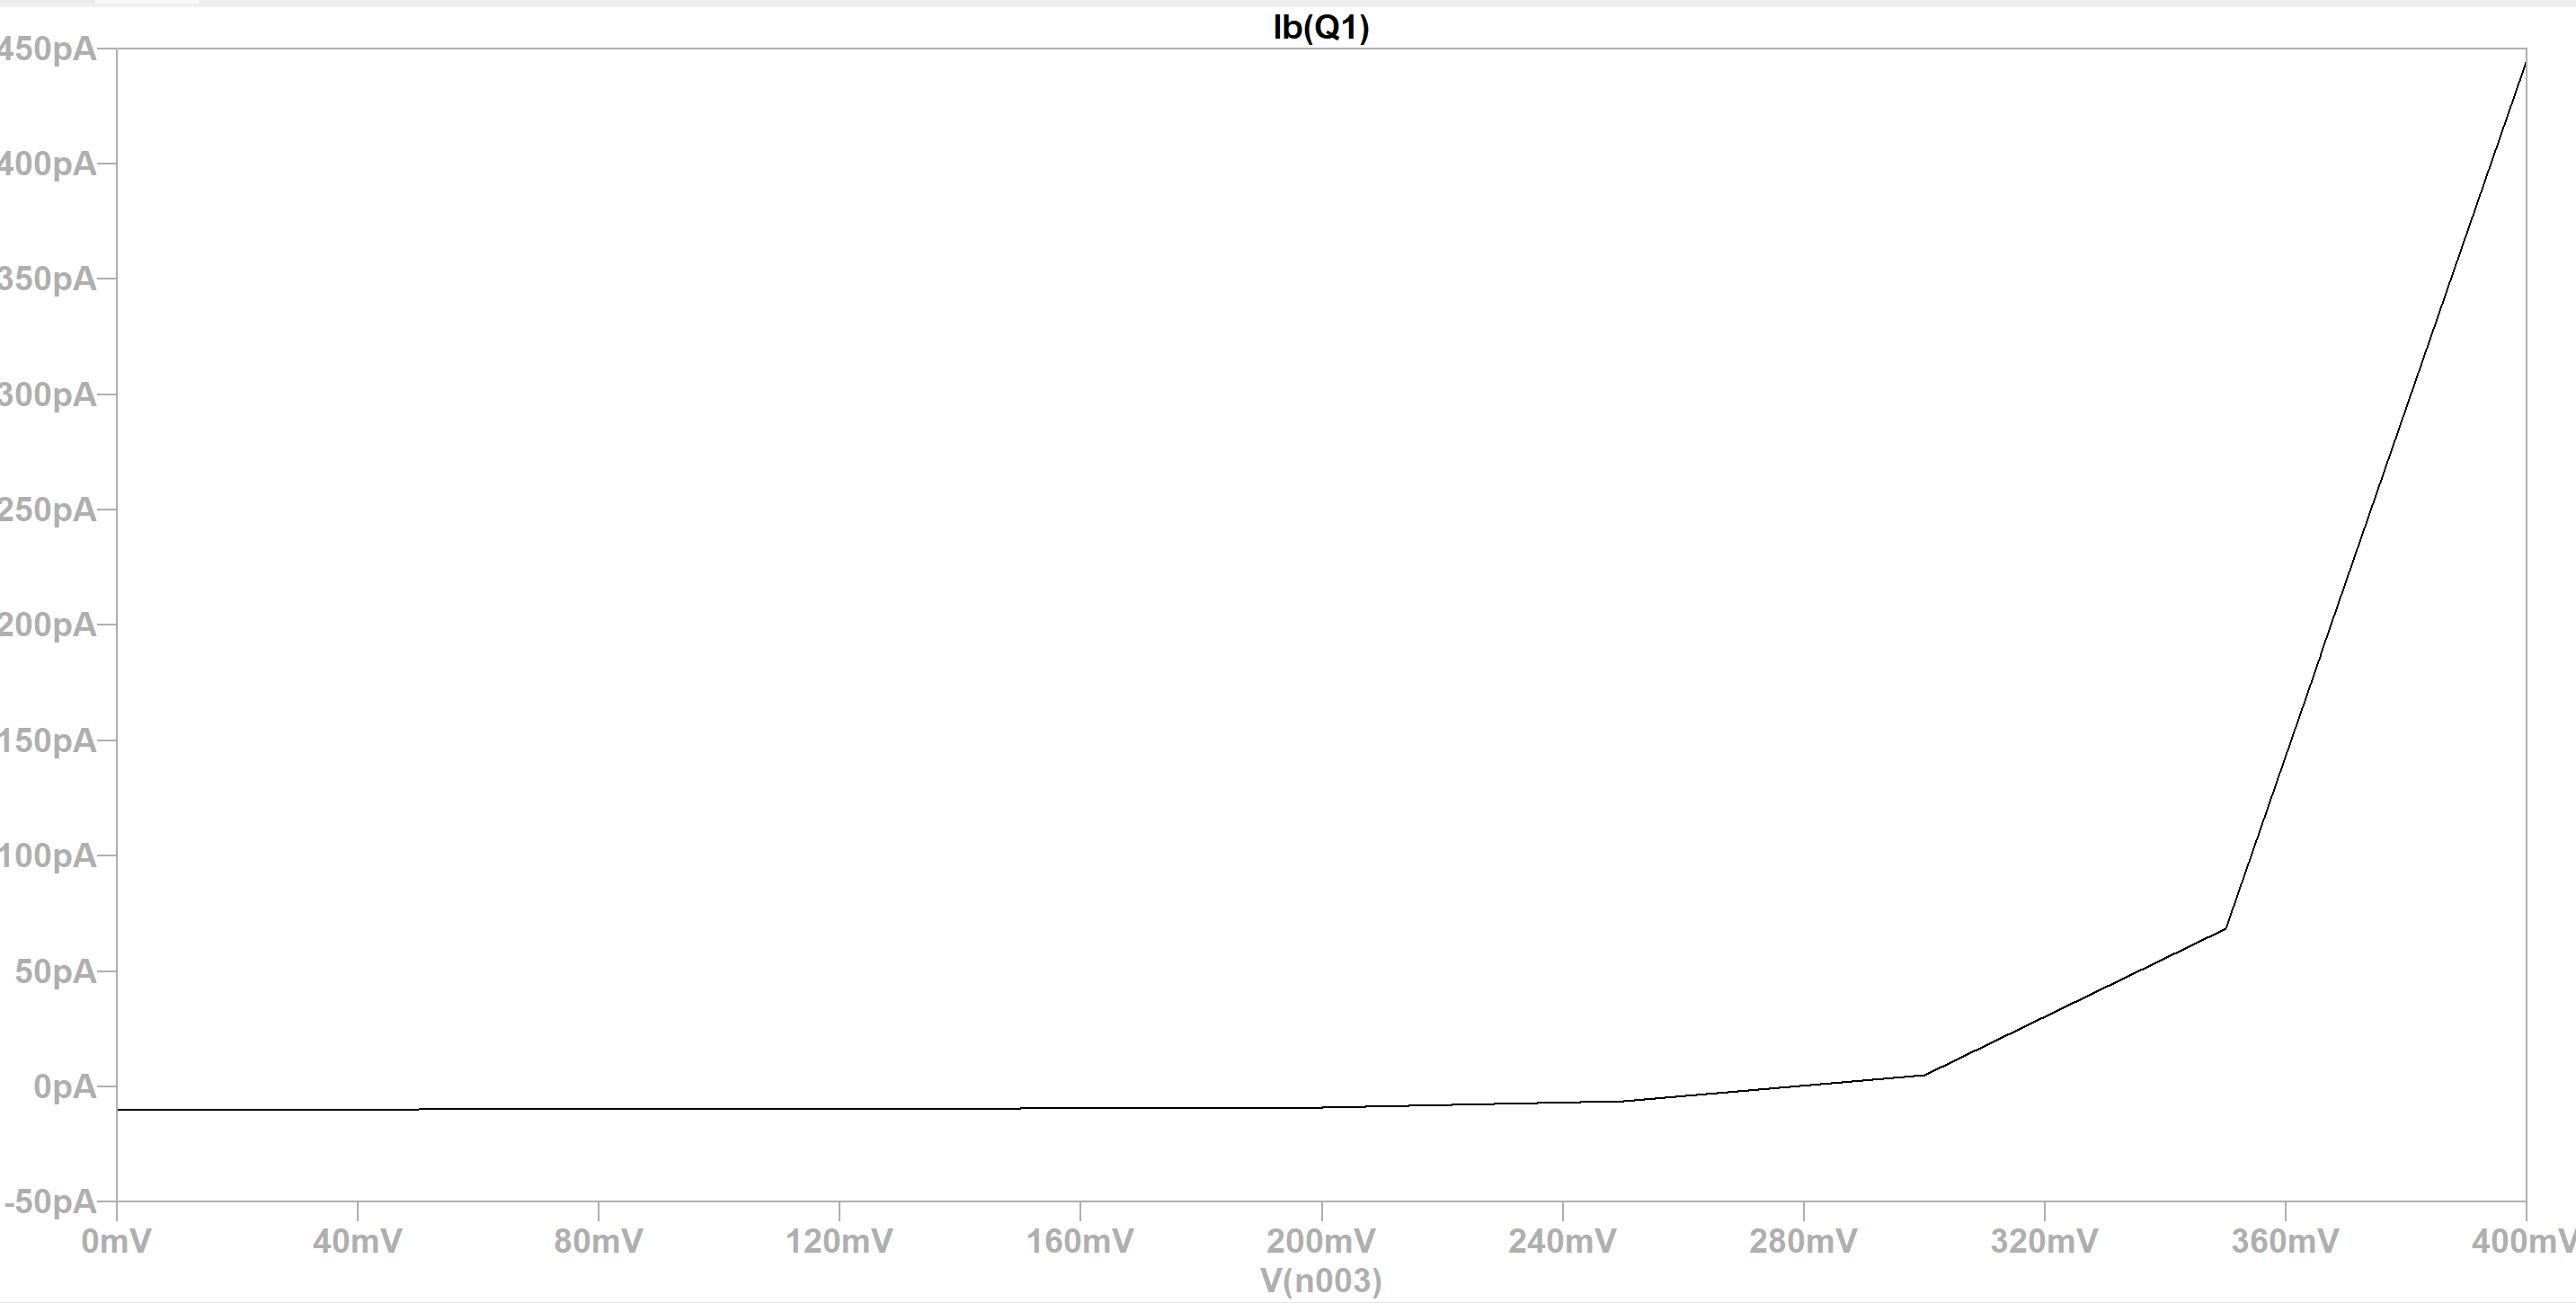
\includegraphics[width=\textwidth]{../CE-Configuration/input/input_0-0.4_VCE=10.png}
        \caption{$0\text{--}0.4\text{ V}$ ($V_{CE} = 10\text{ V}$)}
    \end{subfigure}
    
    \vspace{0.2cm}
    \begin{subfigure}[b]{0.31\textwidth}
        \centering
        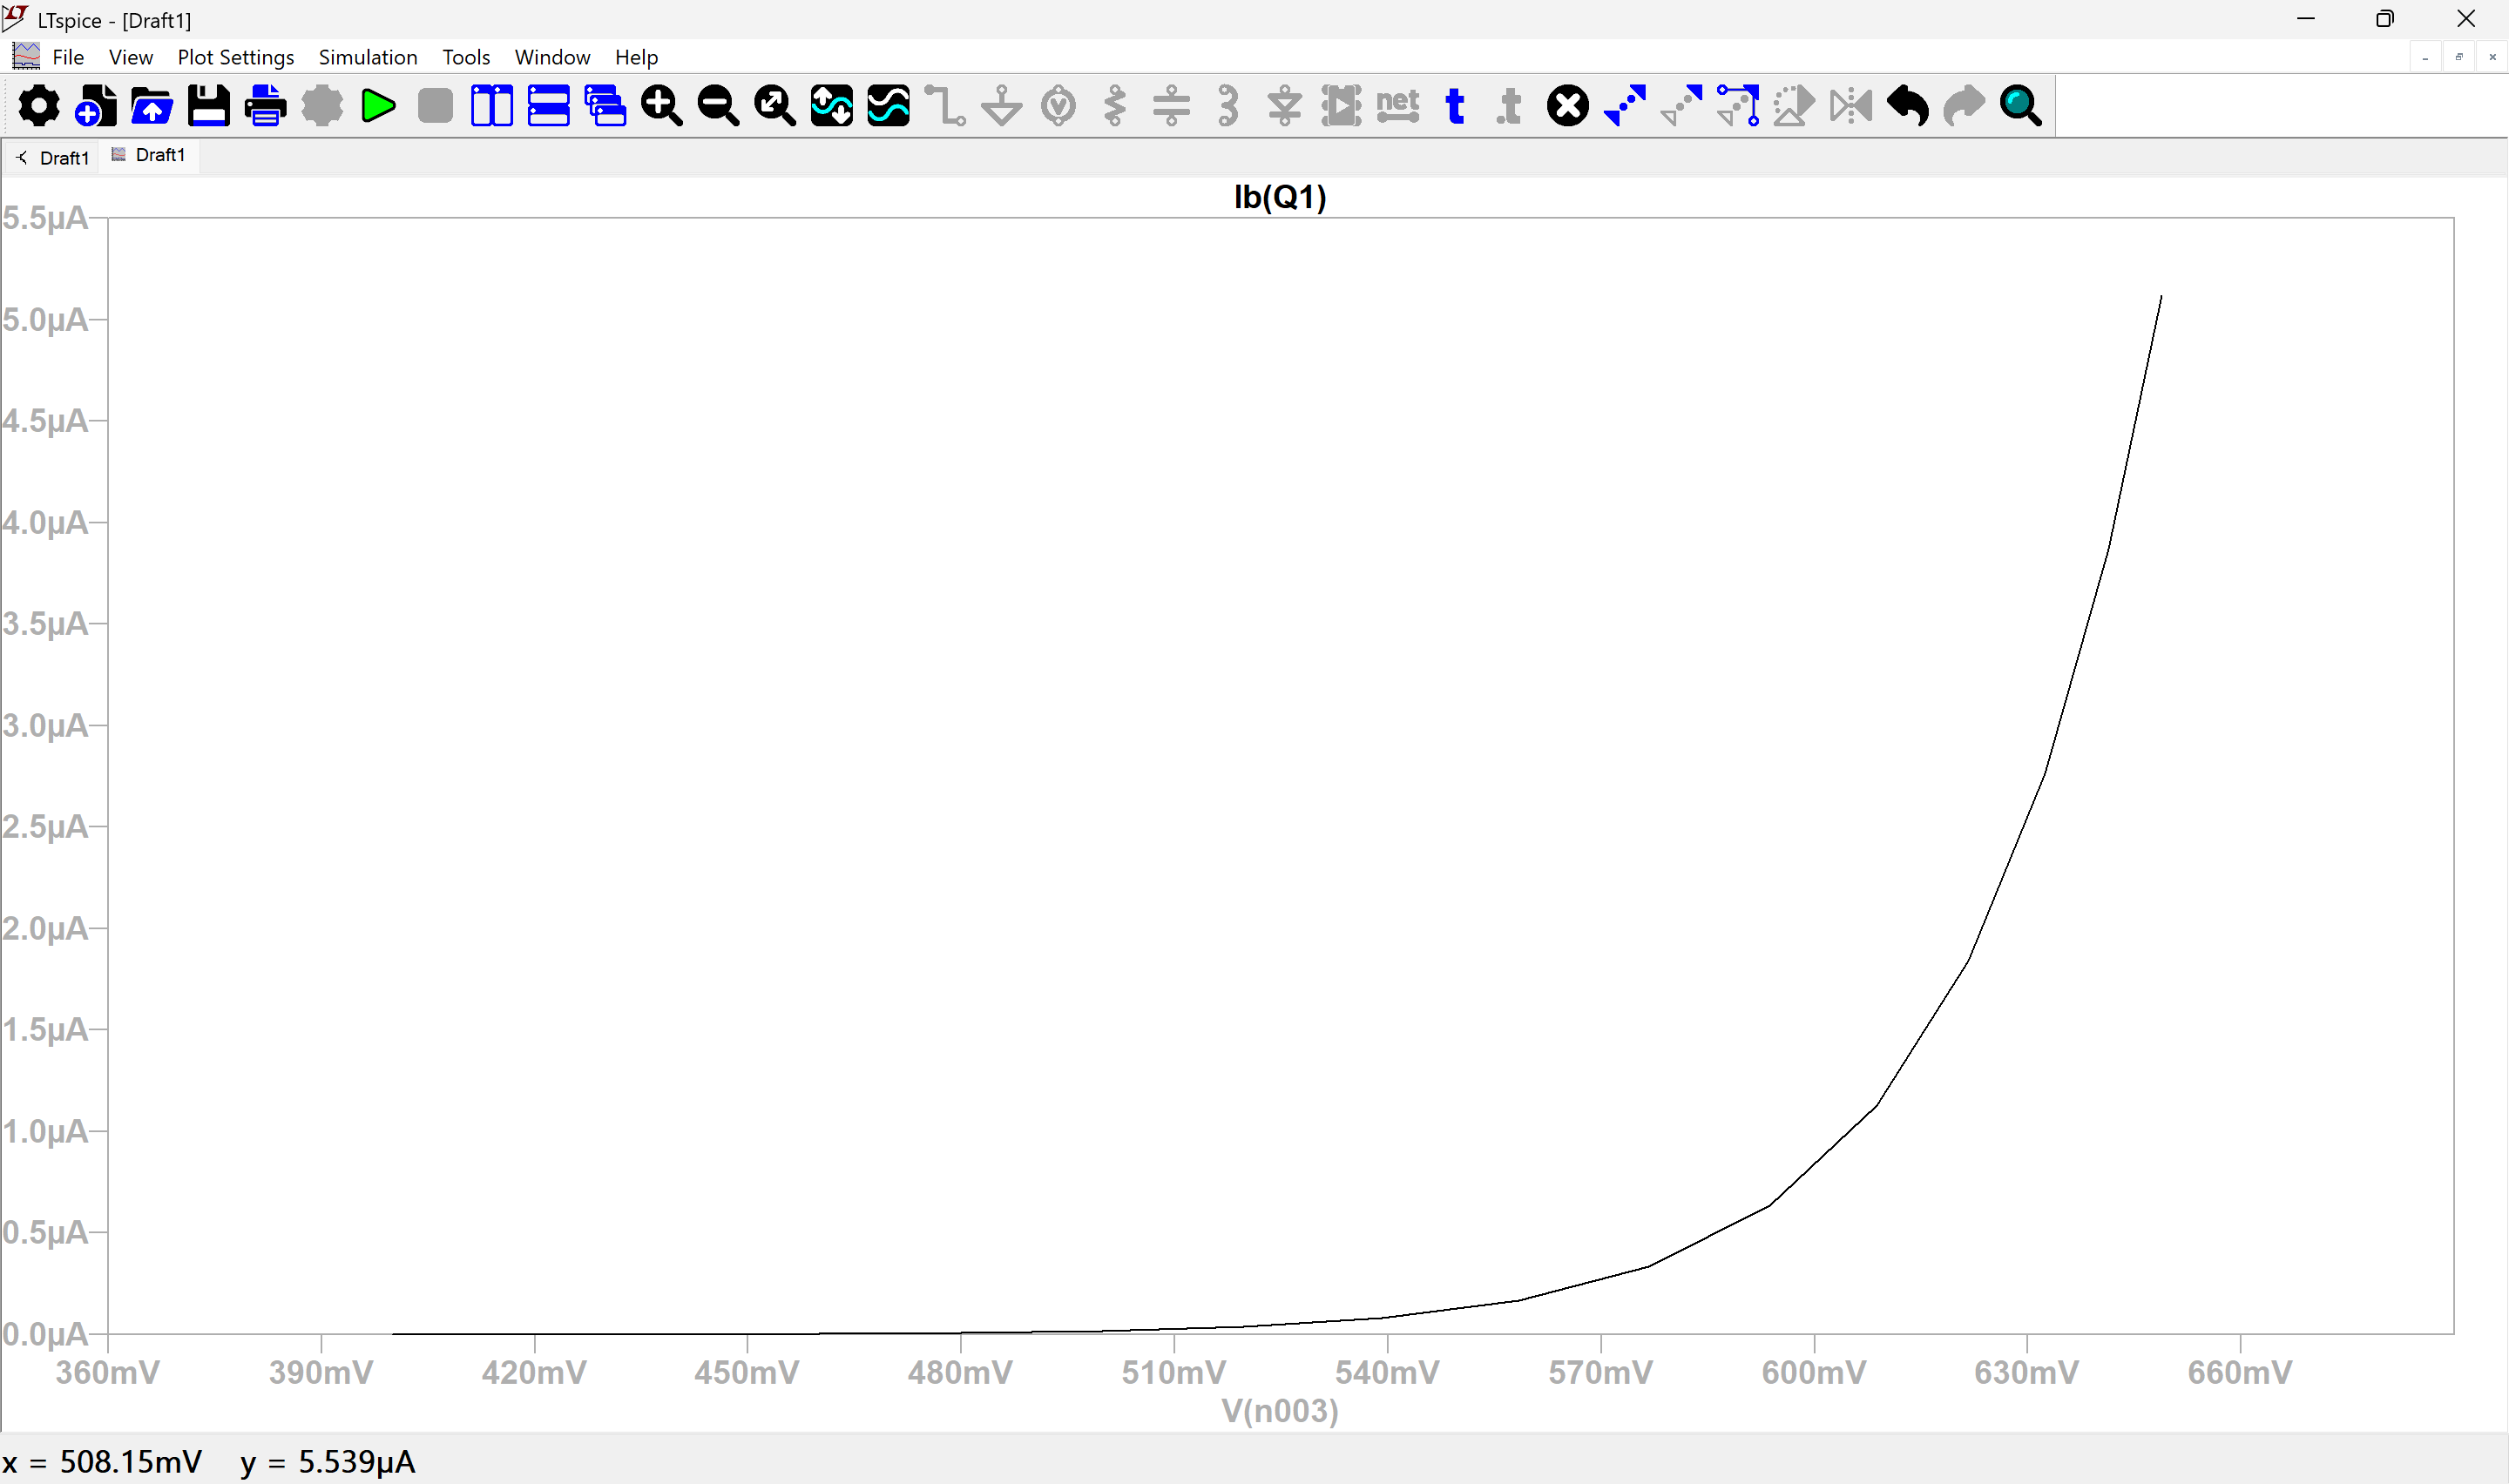
\includegraphics[width=\textwidth]{../CE-Configuration/input/input_0.4-0.7_VCE=1.png}
        \caption{$0.4\text{--}0.7\text{ V}$ ($V_{CE} = 1\text{ V}$)}
    \end{subfigure}
    \hfill
    \begin{subfigure}[b]{0.31\textwidth}
        \centering
        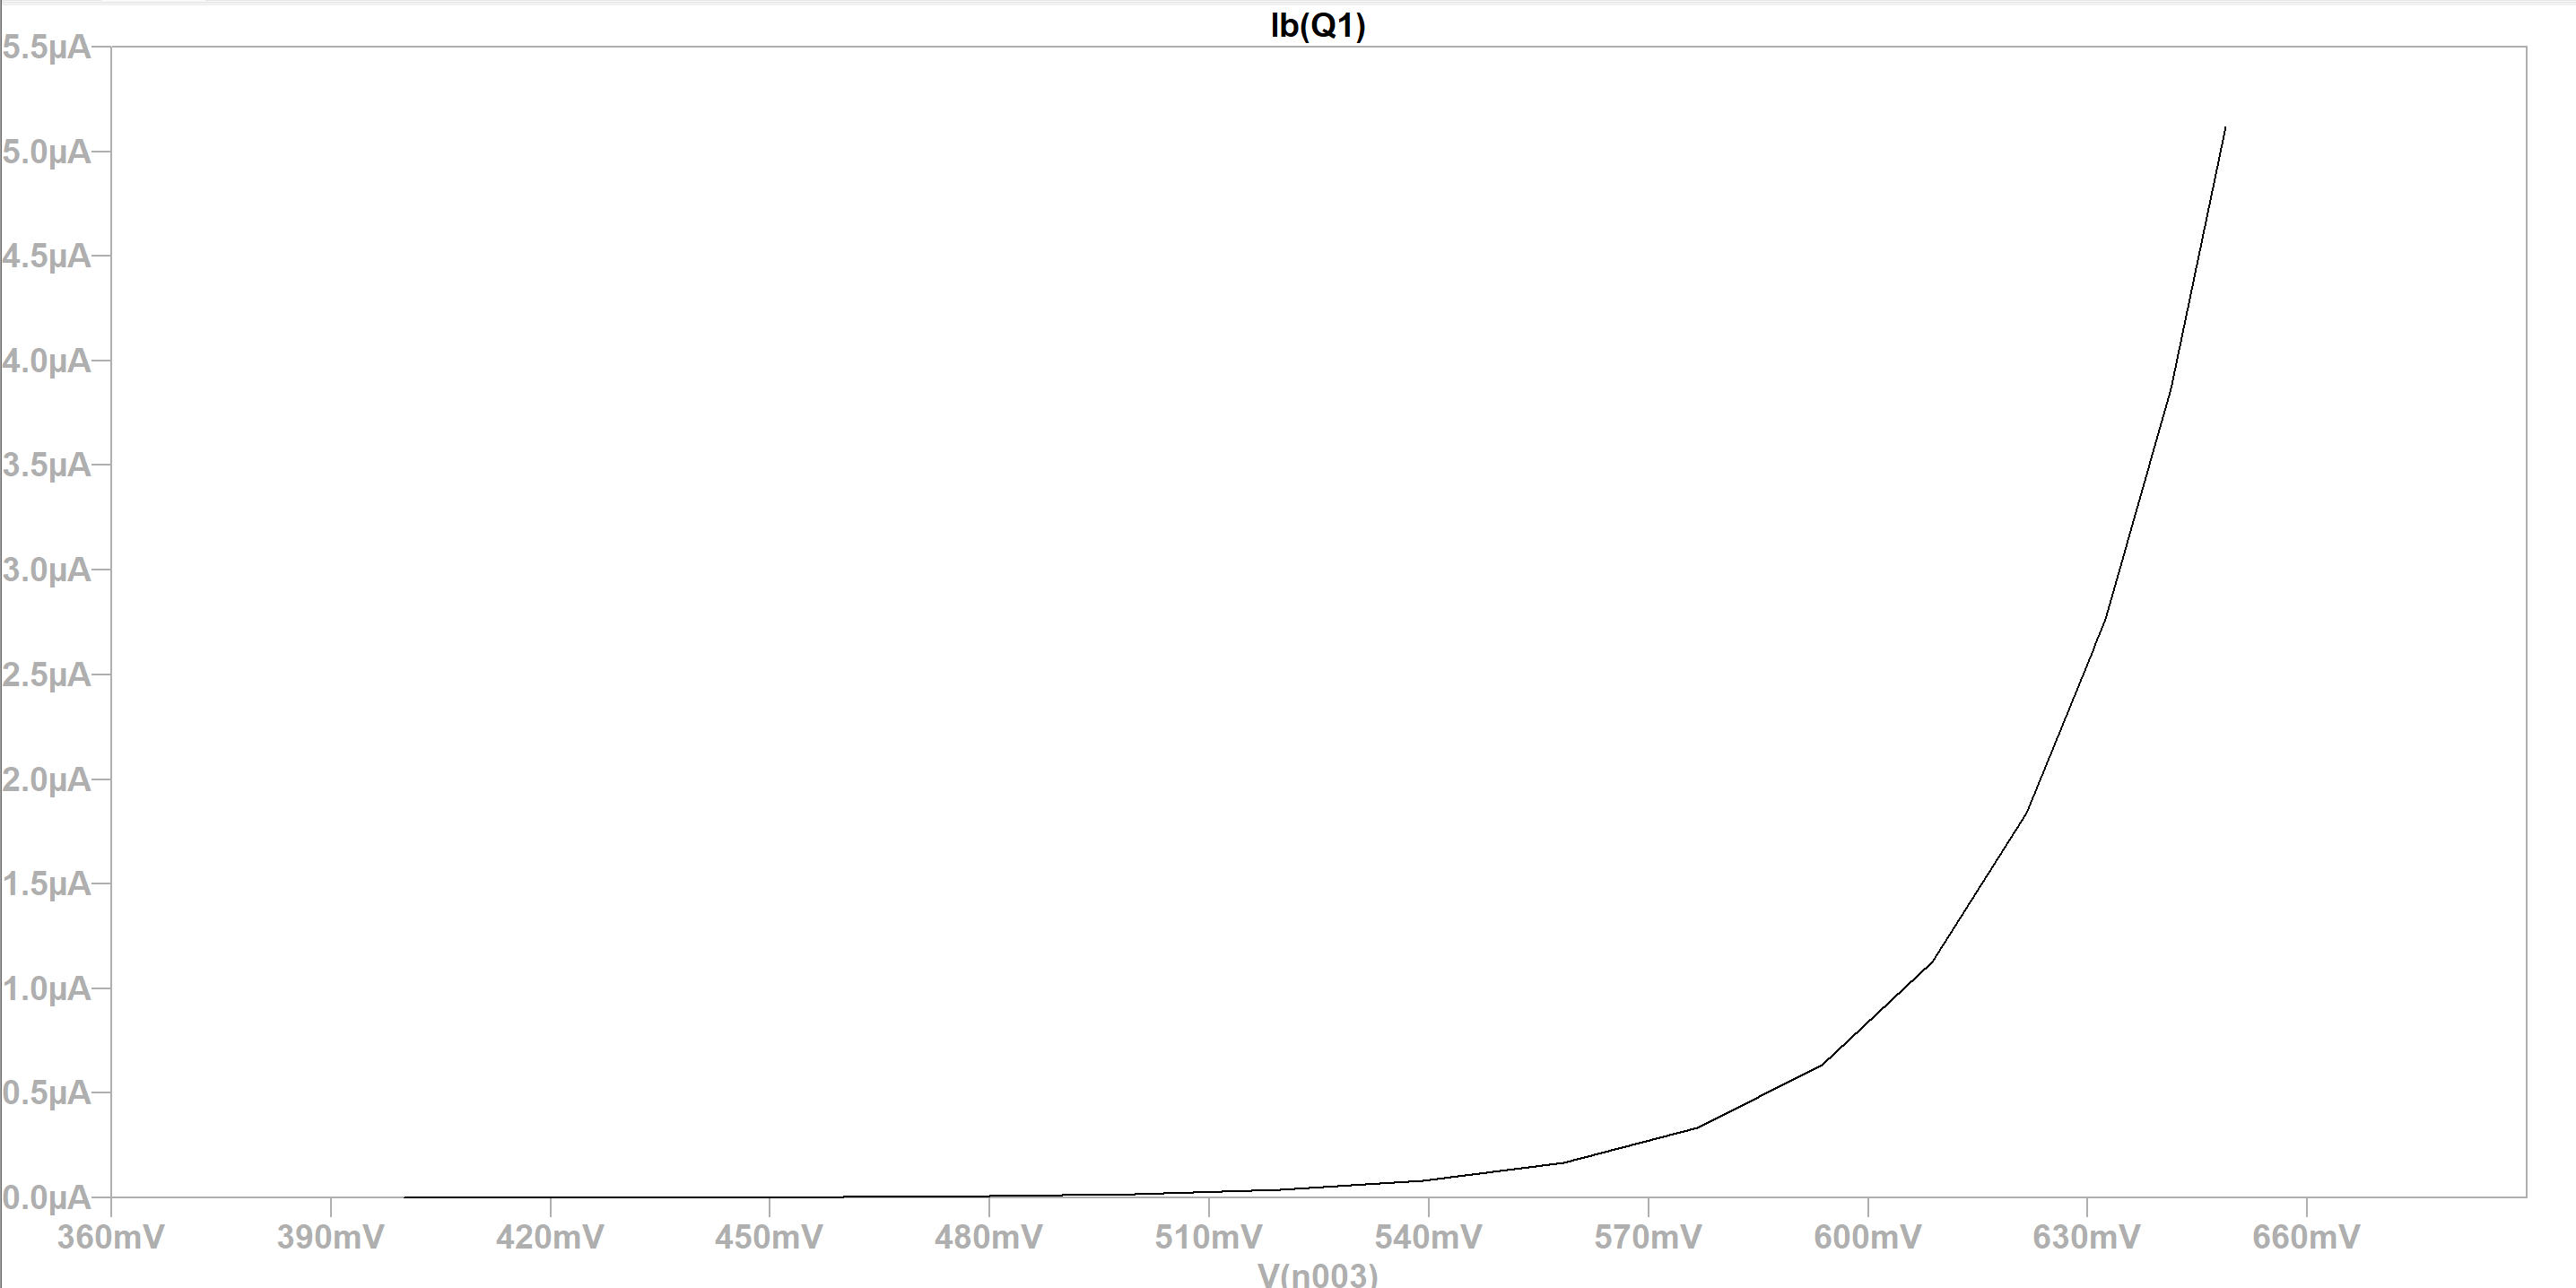
\includegraphics[width=\textwidth]{../CE-Configuration/input/input_0.4-0.7_VCE=5.png}
        \caption{$0.4\text{--}0.7\text{ V}$ ($V_{CE} = 5\text{ V}$)}
    \end{subfigure}
    \hfill
    \begin{subfigure}[b]{0.31\textwidth}
        \centering
        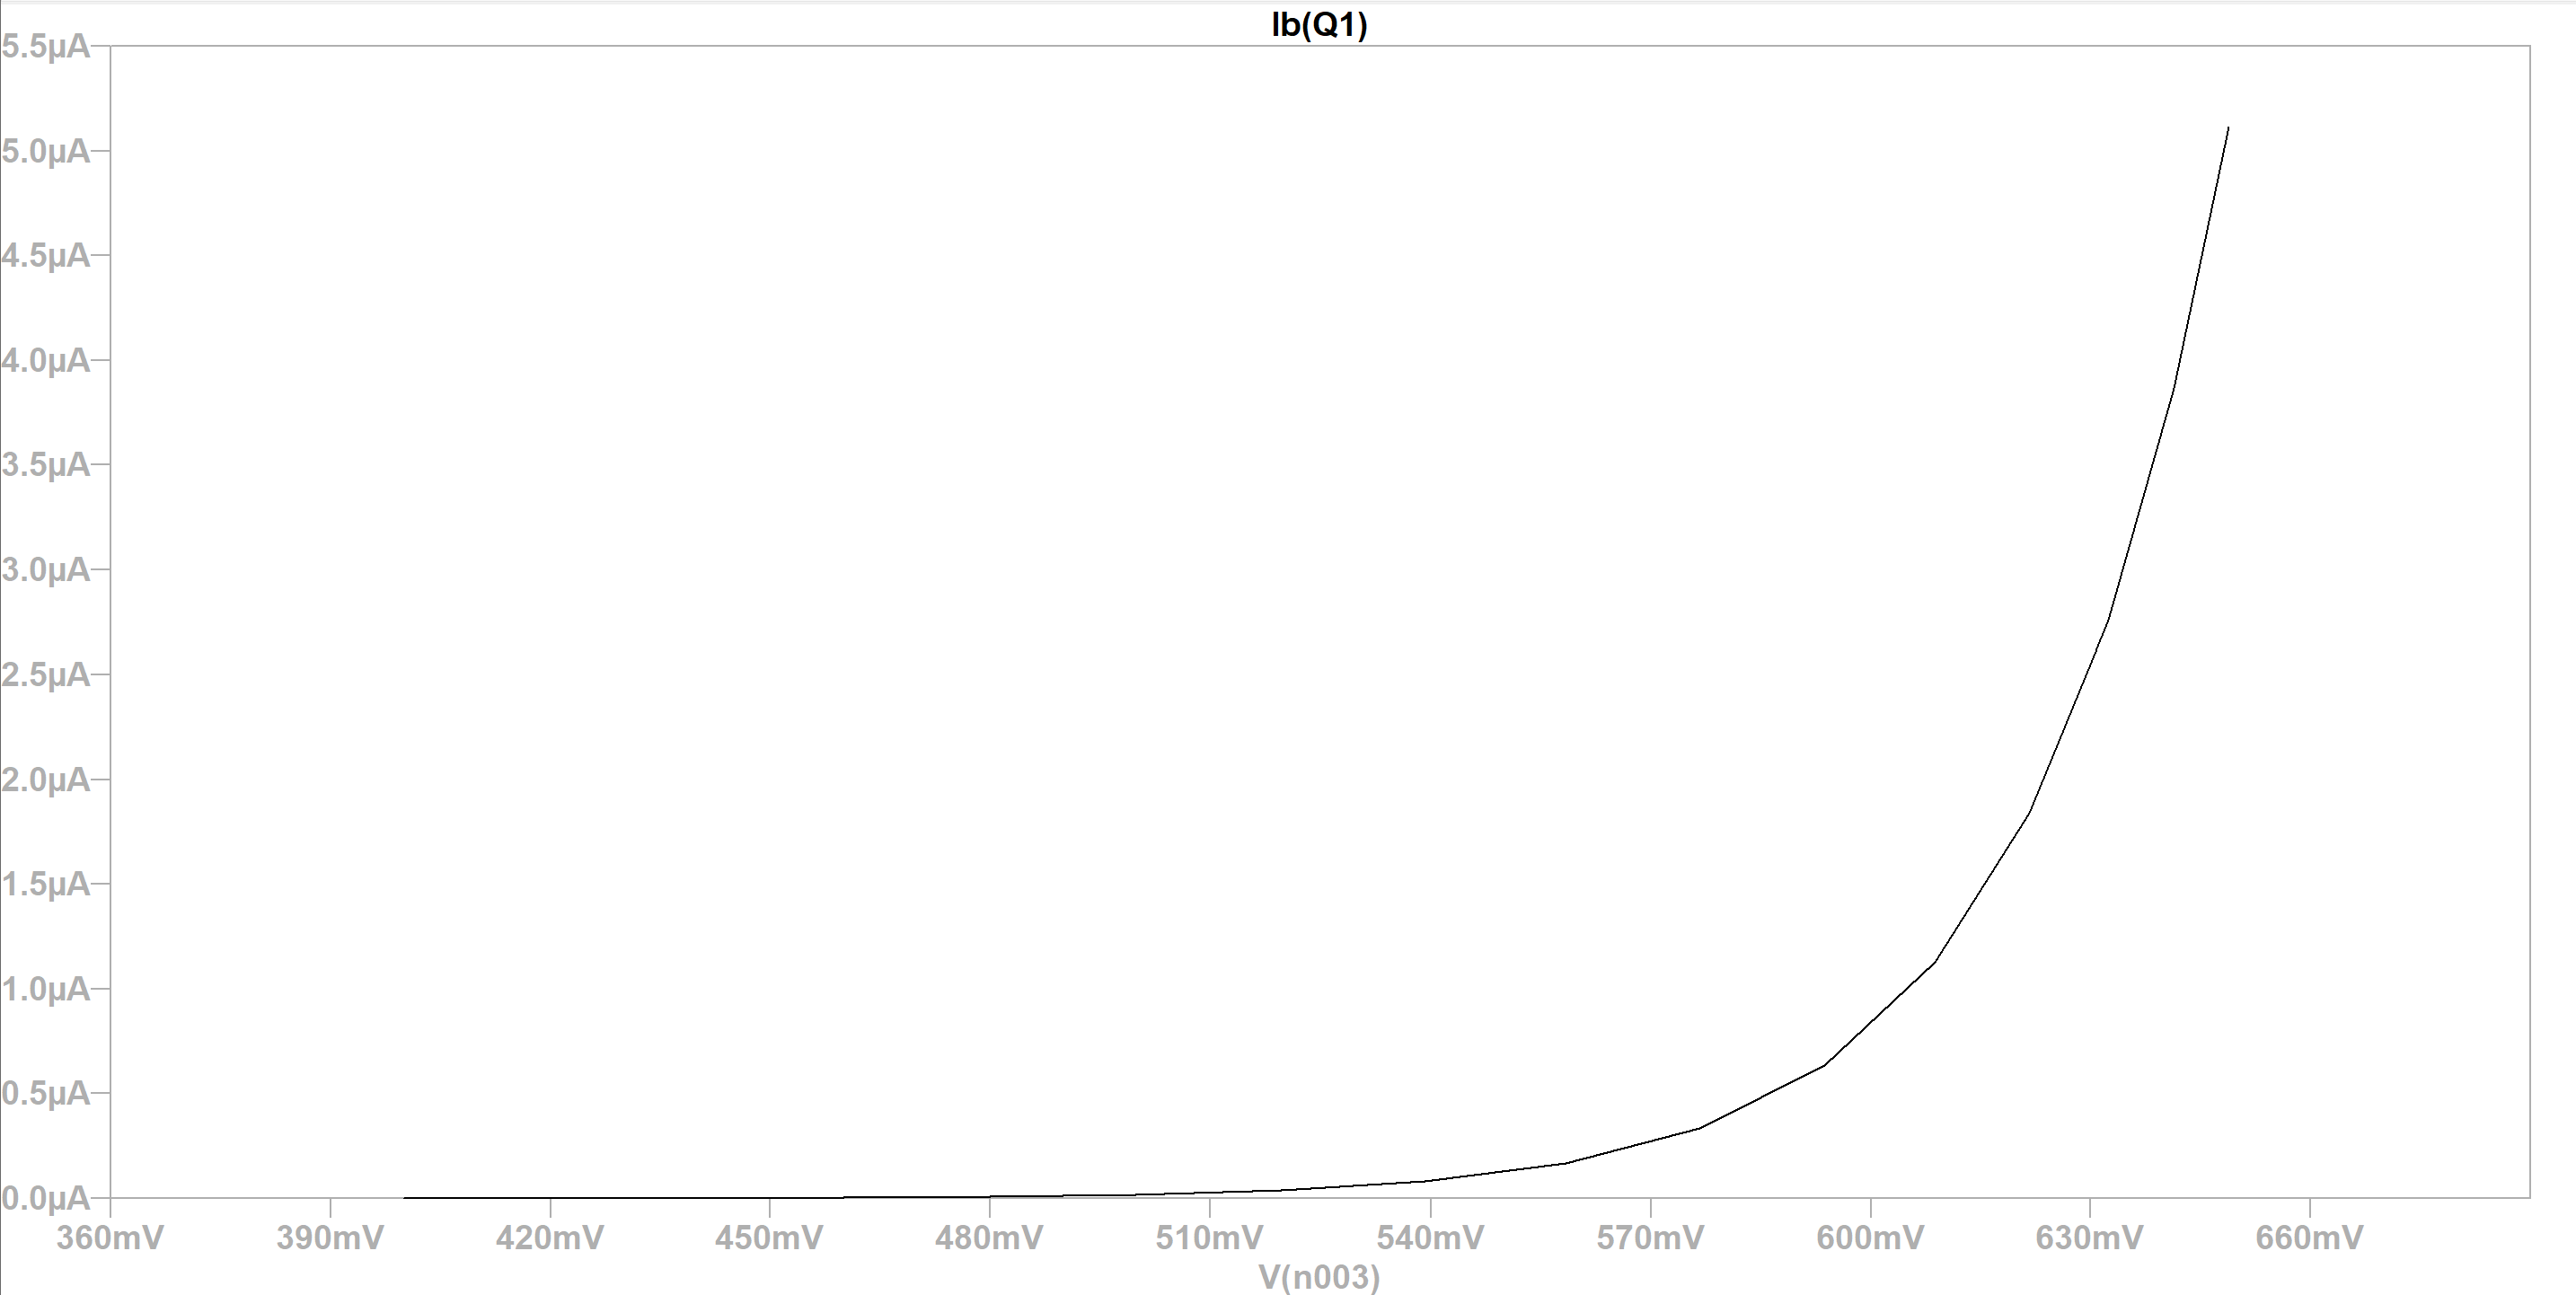
\includegraphics[width=\textwidth]{../CE-Configuration/input/input_0.4-0.7_VCE=10.png}
        \caption{$0.4\text{--}0.7\text{ V}$ ($V_{CE} = 10\text{ V}$)}
    \end{subfigure}
    \caption{LTspice Simulation of CE Input Characteristics ($I_B$ vs $V_{BE}$) for $V_{CE} = 1\text{ V}, 5\text{ V}, 10\text{ V}$.}
    \label{fig:ce_input_sim}
\end{figure}

\subsubsection{CE Output Characteristics Simulation}
\begin{figure}[H]
    \centering
    \begin{subfigure}[b]{0.31\textwidth}
        \centering
        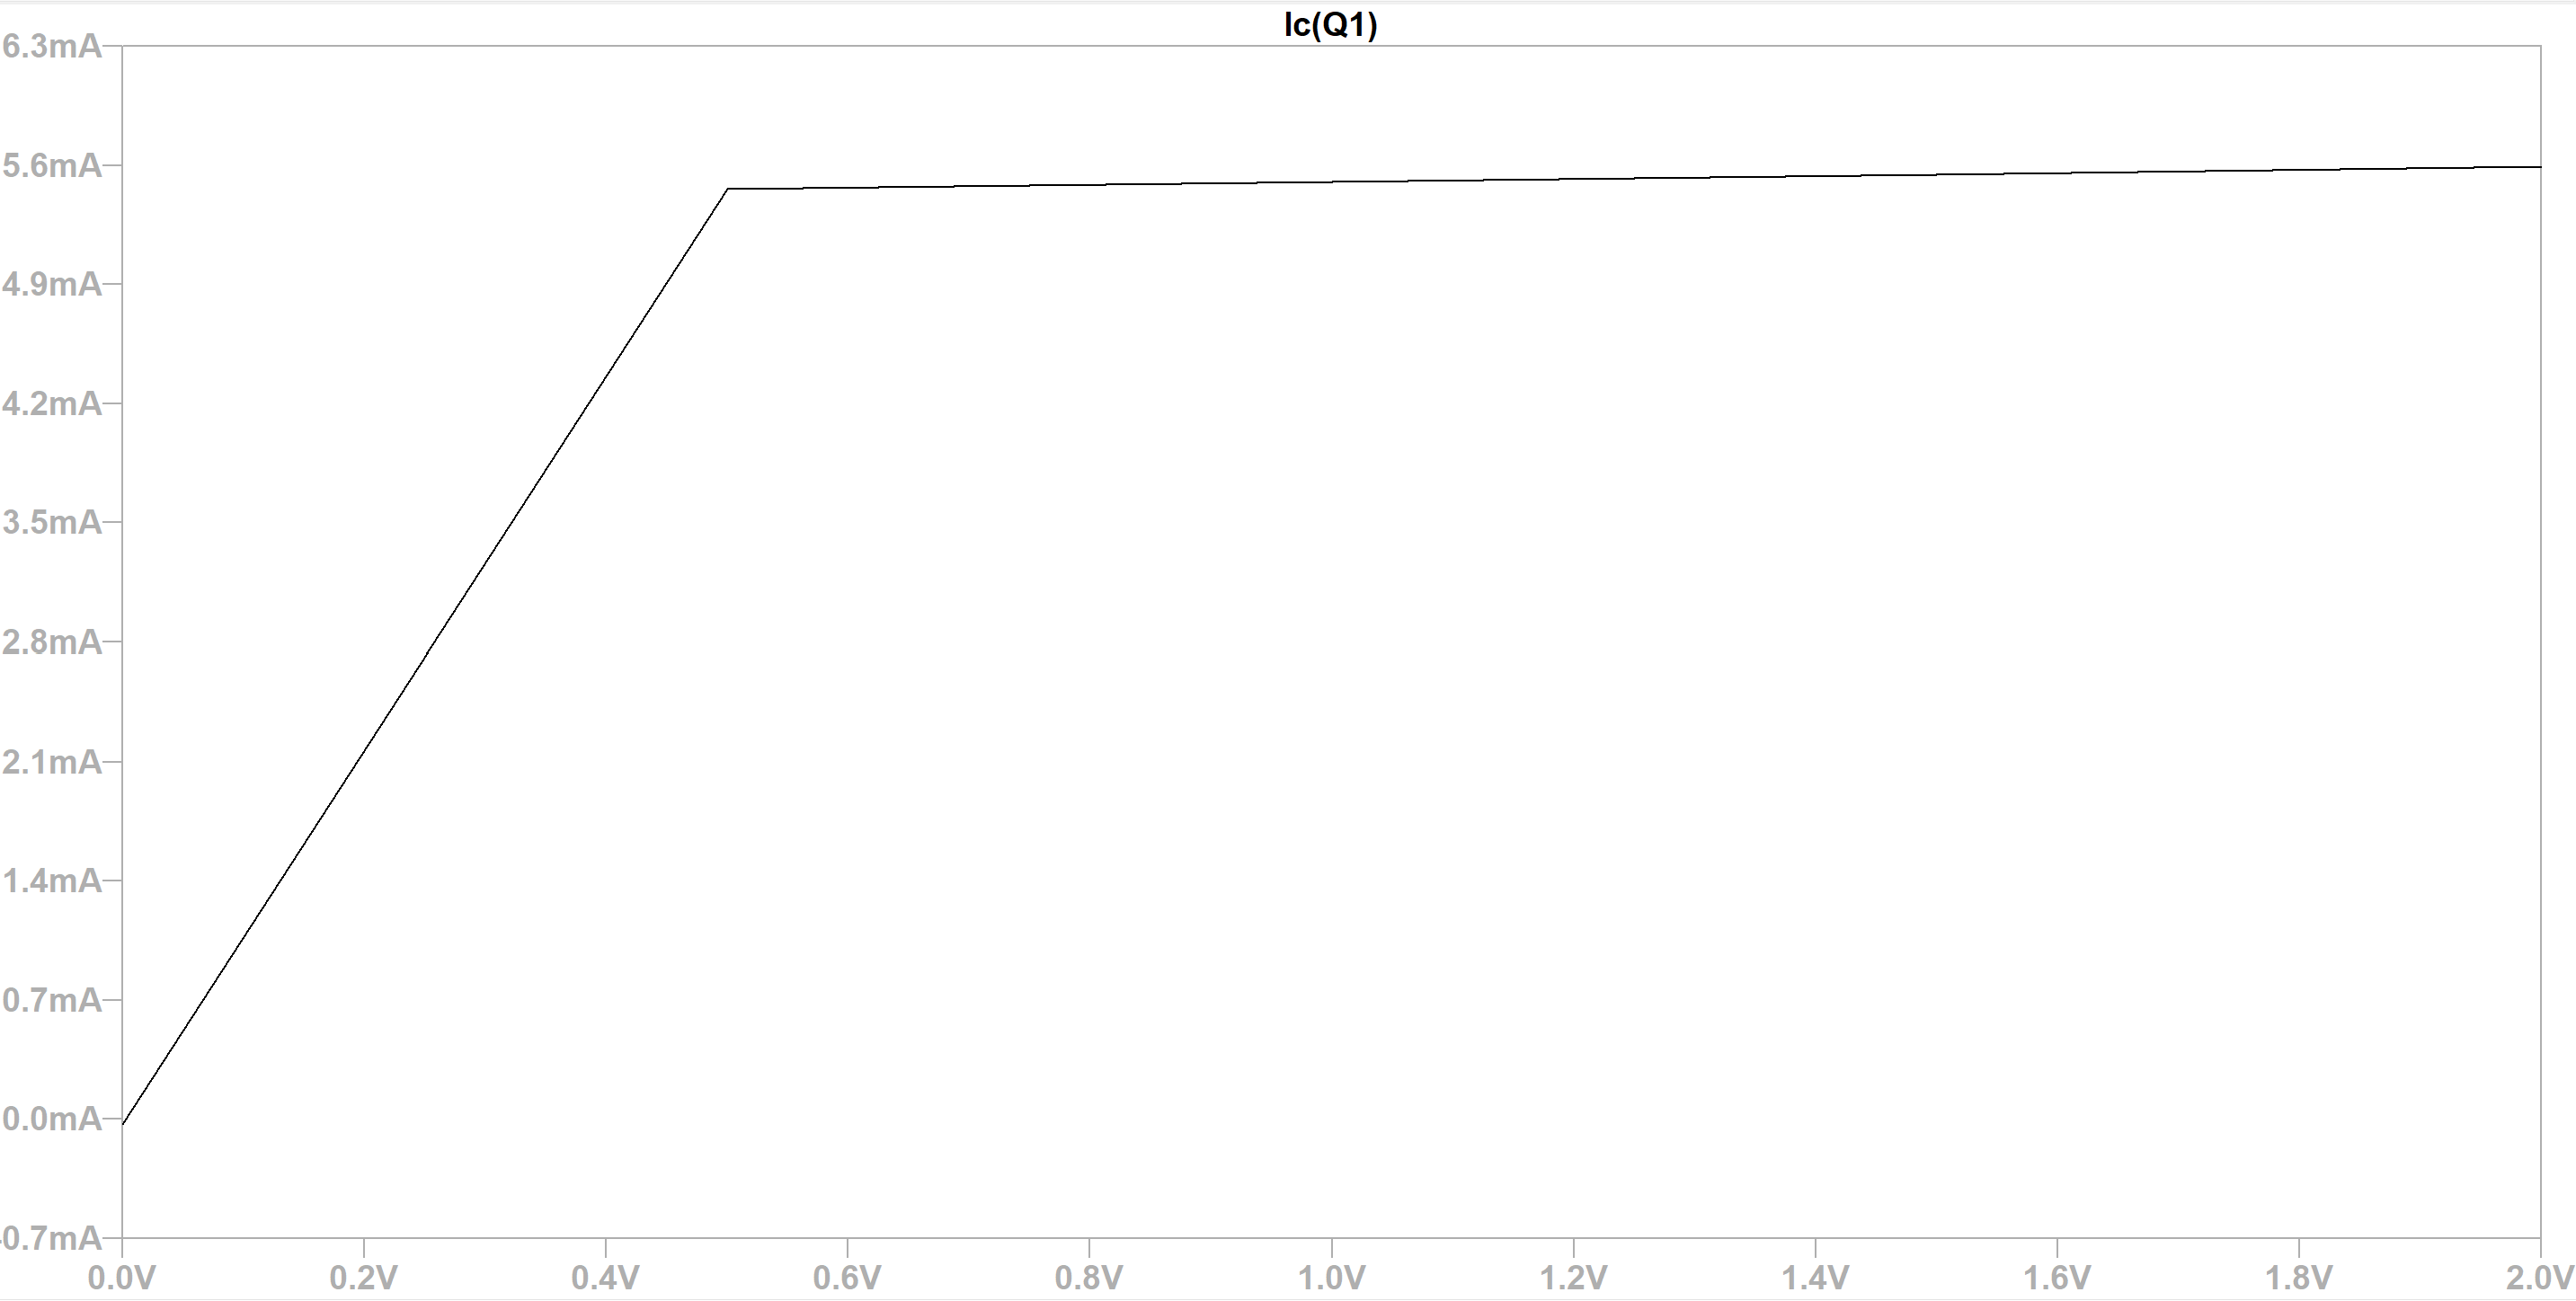
\includegraphics[width=\textwidth]{../CE-Configuration/output/output_0-2_IB=20u.png}
        \caption{$V_{CE}=0\text{--}2\text{V}$, $I_B=20\mu\text{A}$}
    \end{subfigure}
    \hfill
    \begin{subfigure}[b]{0.31\textwidth}
        \centering
        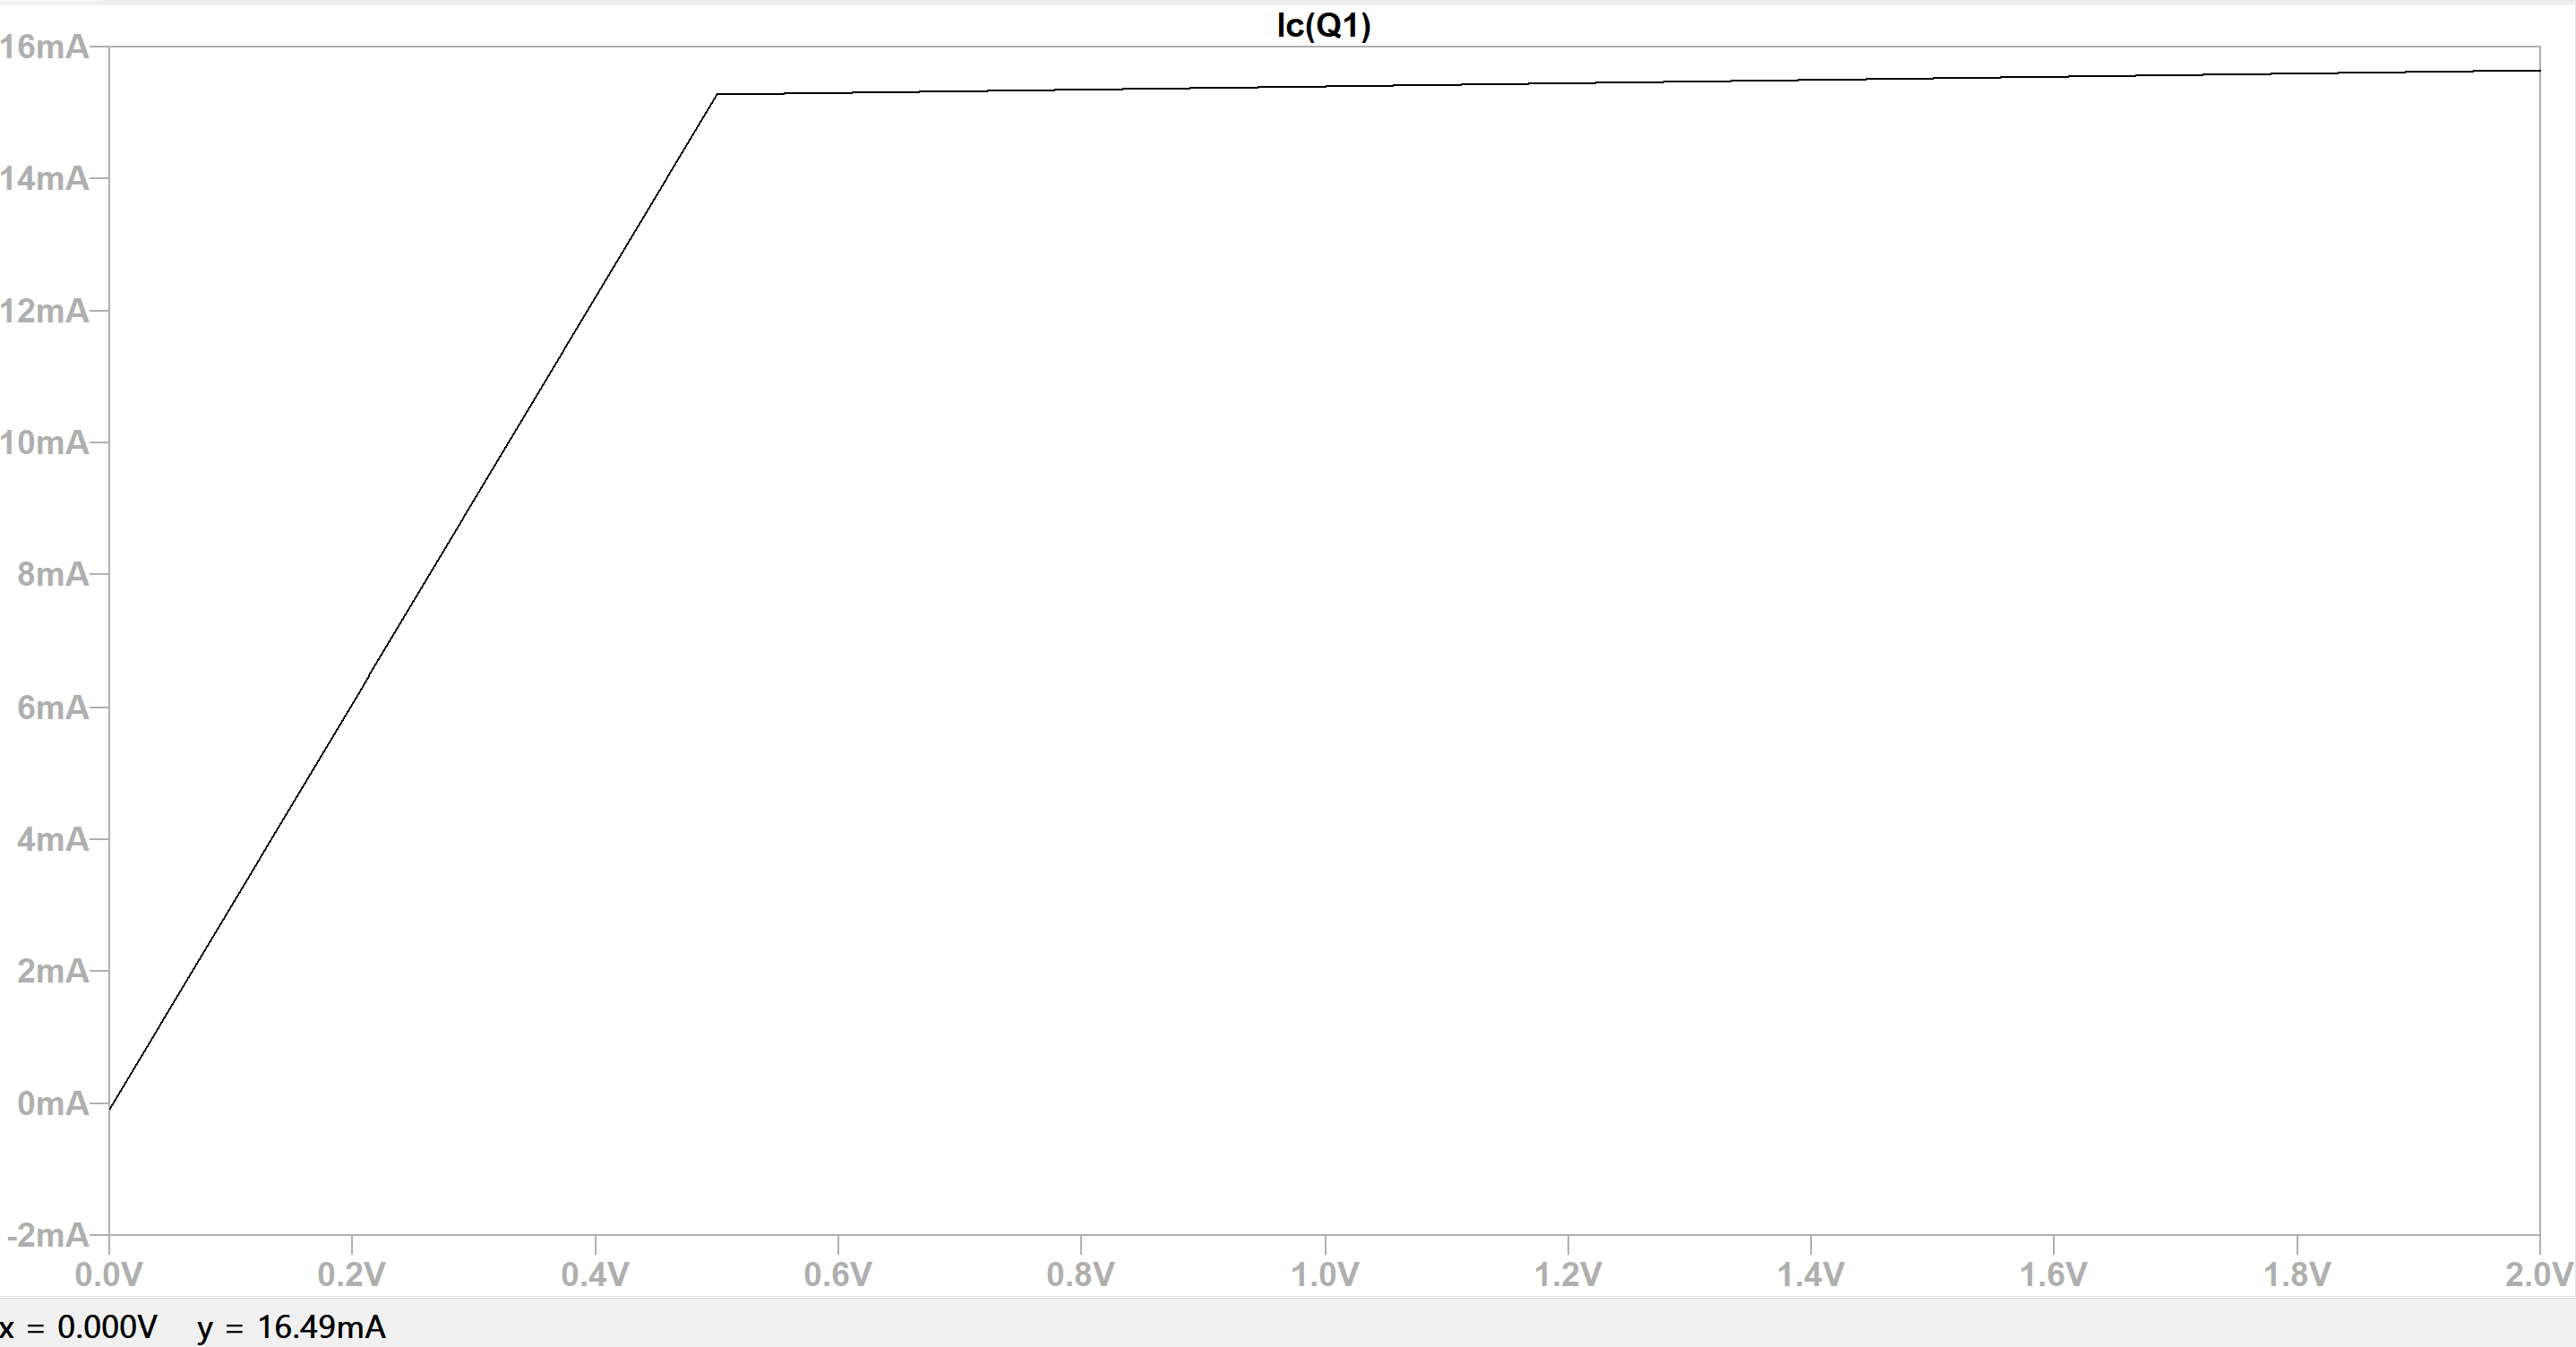
\includegraphics[width=\textwidth]{../CE-Configuration/output/output_0-2_IB=60u.png}
        \caption{$V_{CE}=0\text{--}2\text{V}$, $I_B=60\mu\text{A}$}
    \end{subfigure}
    \hfill
    \begin{subfigure}[b]{0.31\textwidth}
        \centering
        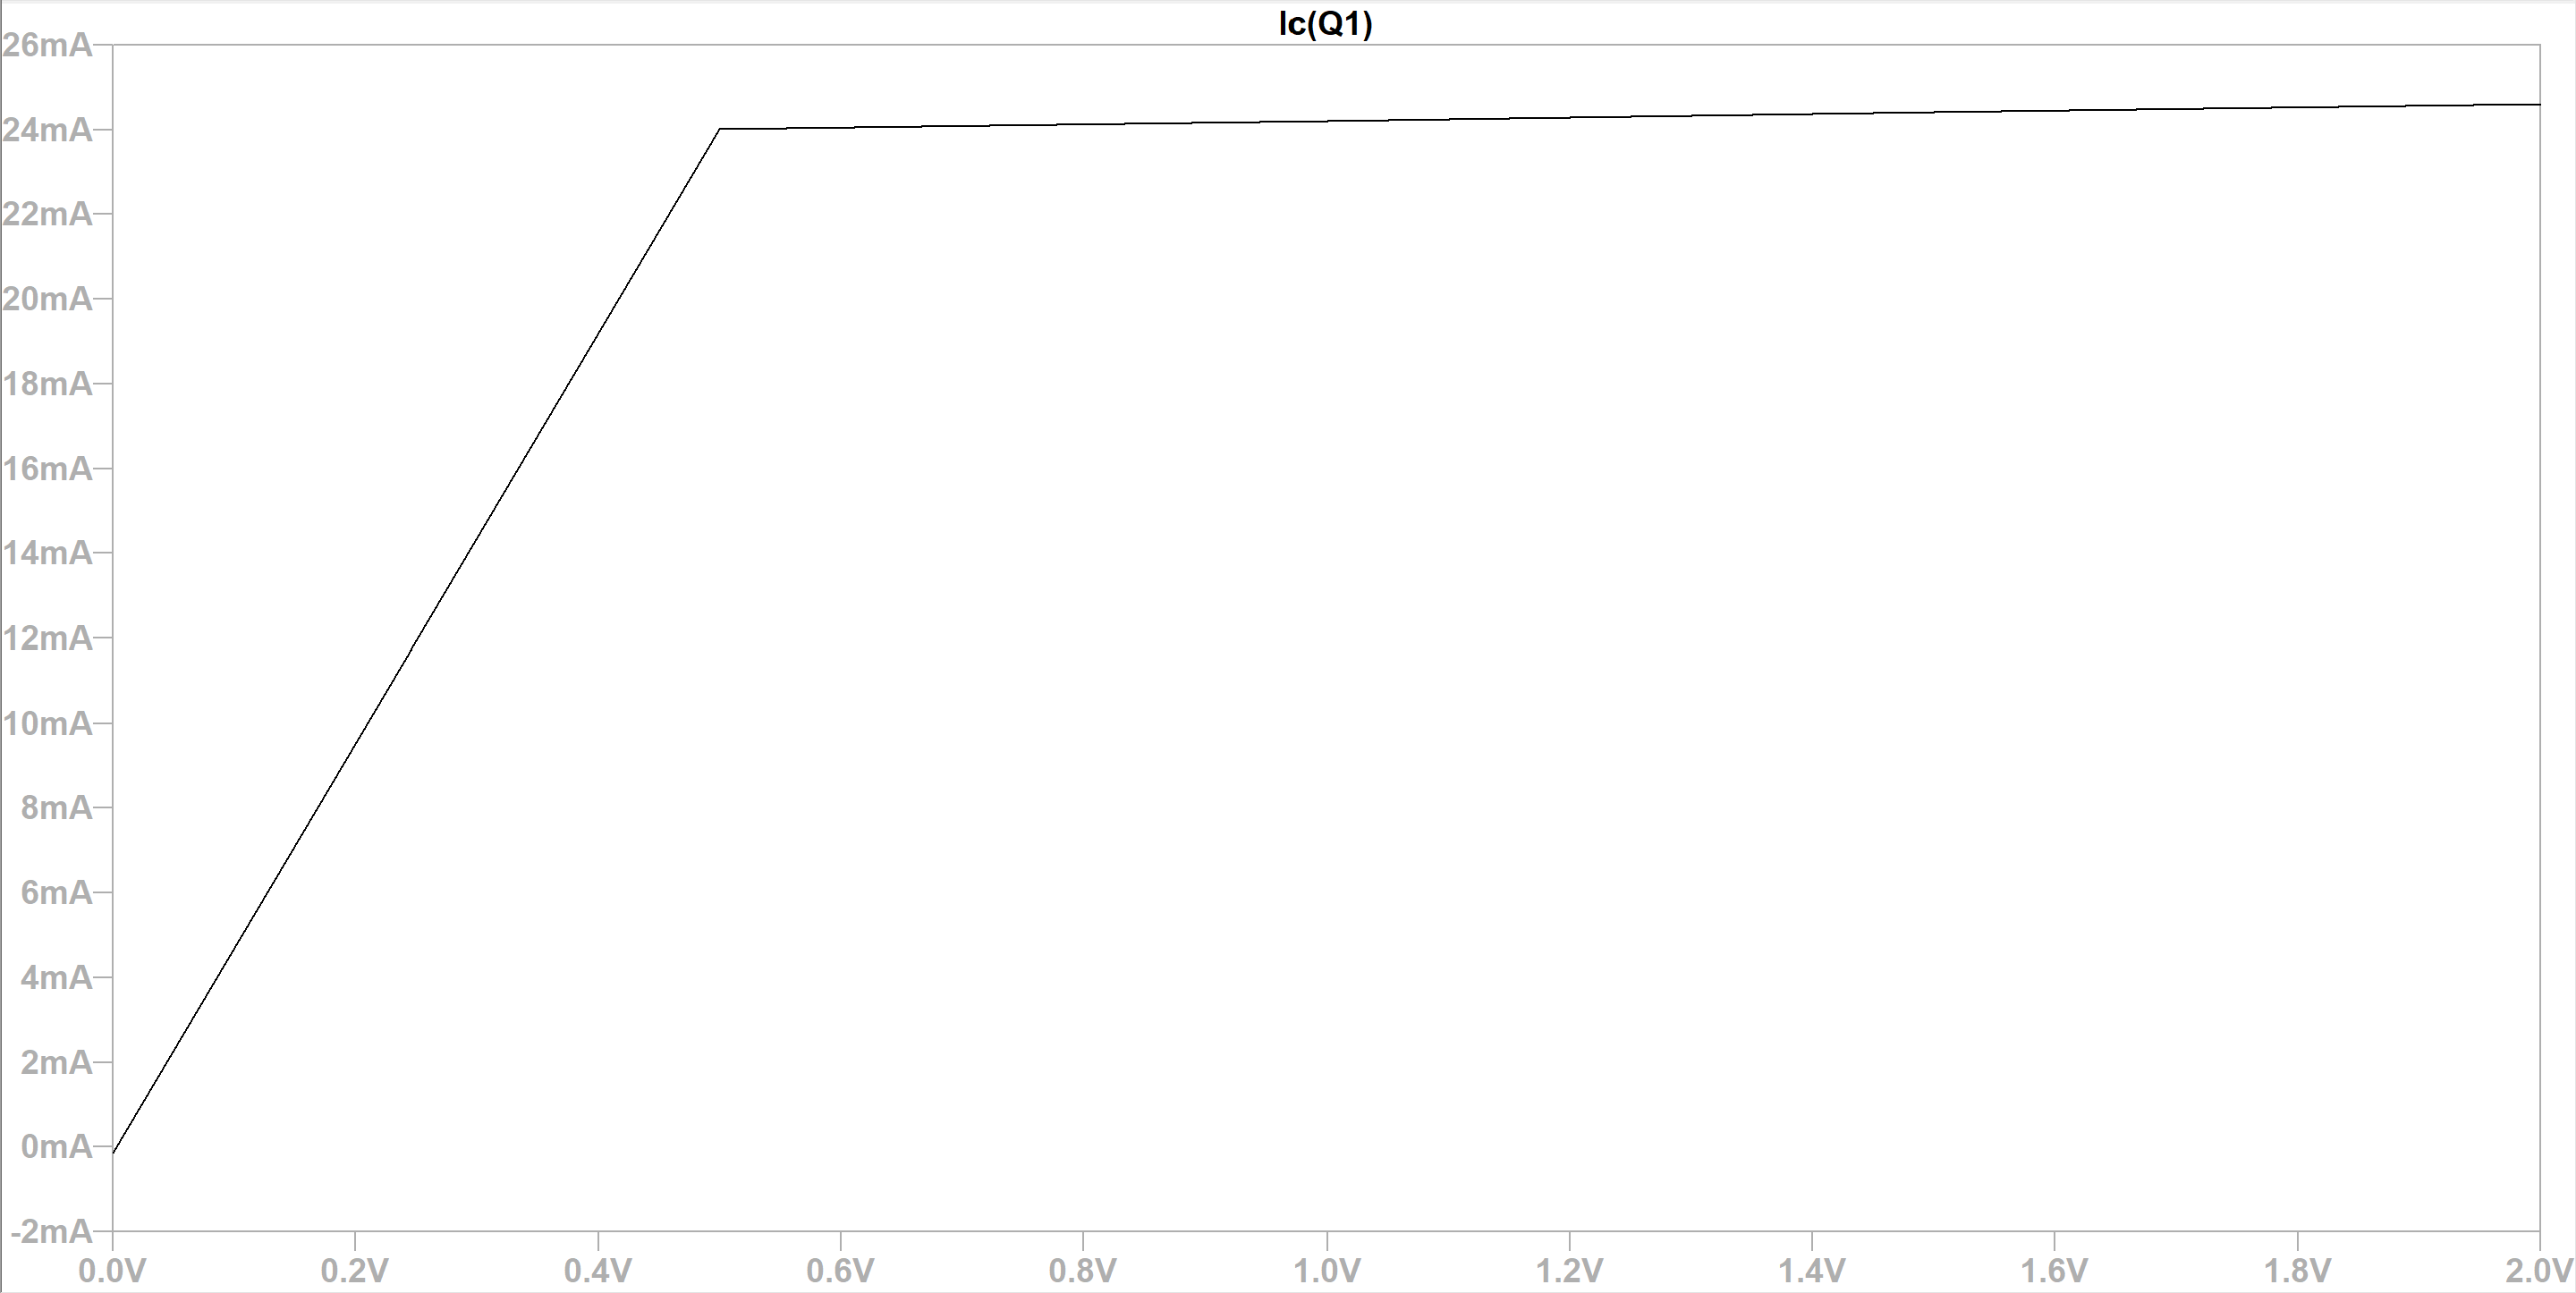
\includegraphics[width=\textwidth]{../CE-Configuration/output/output_0-2_IB=100u.png}
        \caption{$V_{CE}=0\text{--}2\text{V}$, $I_B=100\mu\text{A}$}
    \end{subfigure}

    \vspace{0.2cm}
    \begin{subfigure}[b]{0.31\textwidth}
        \centering
        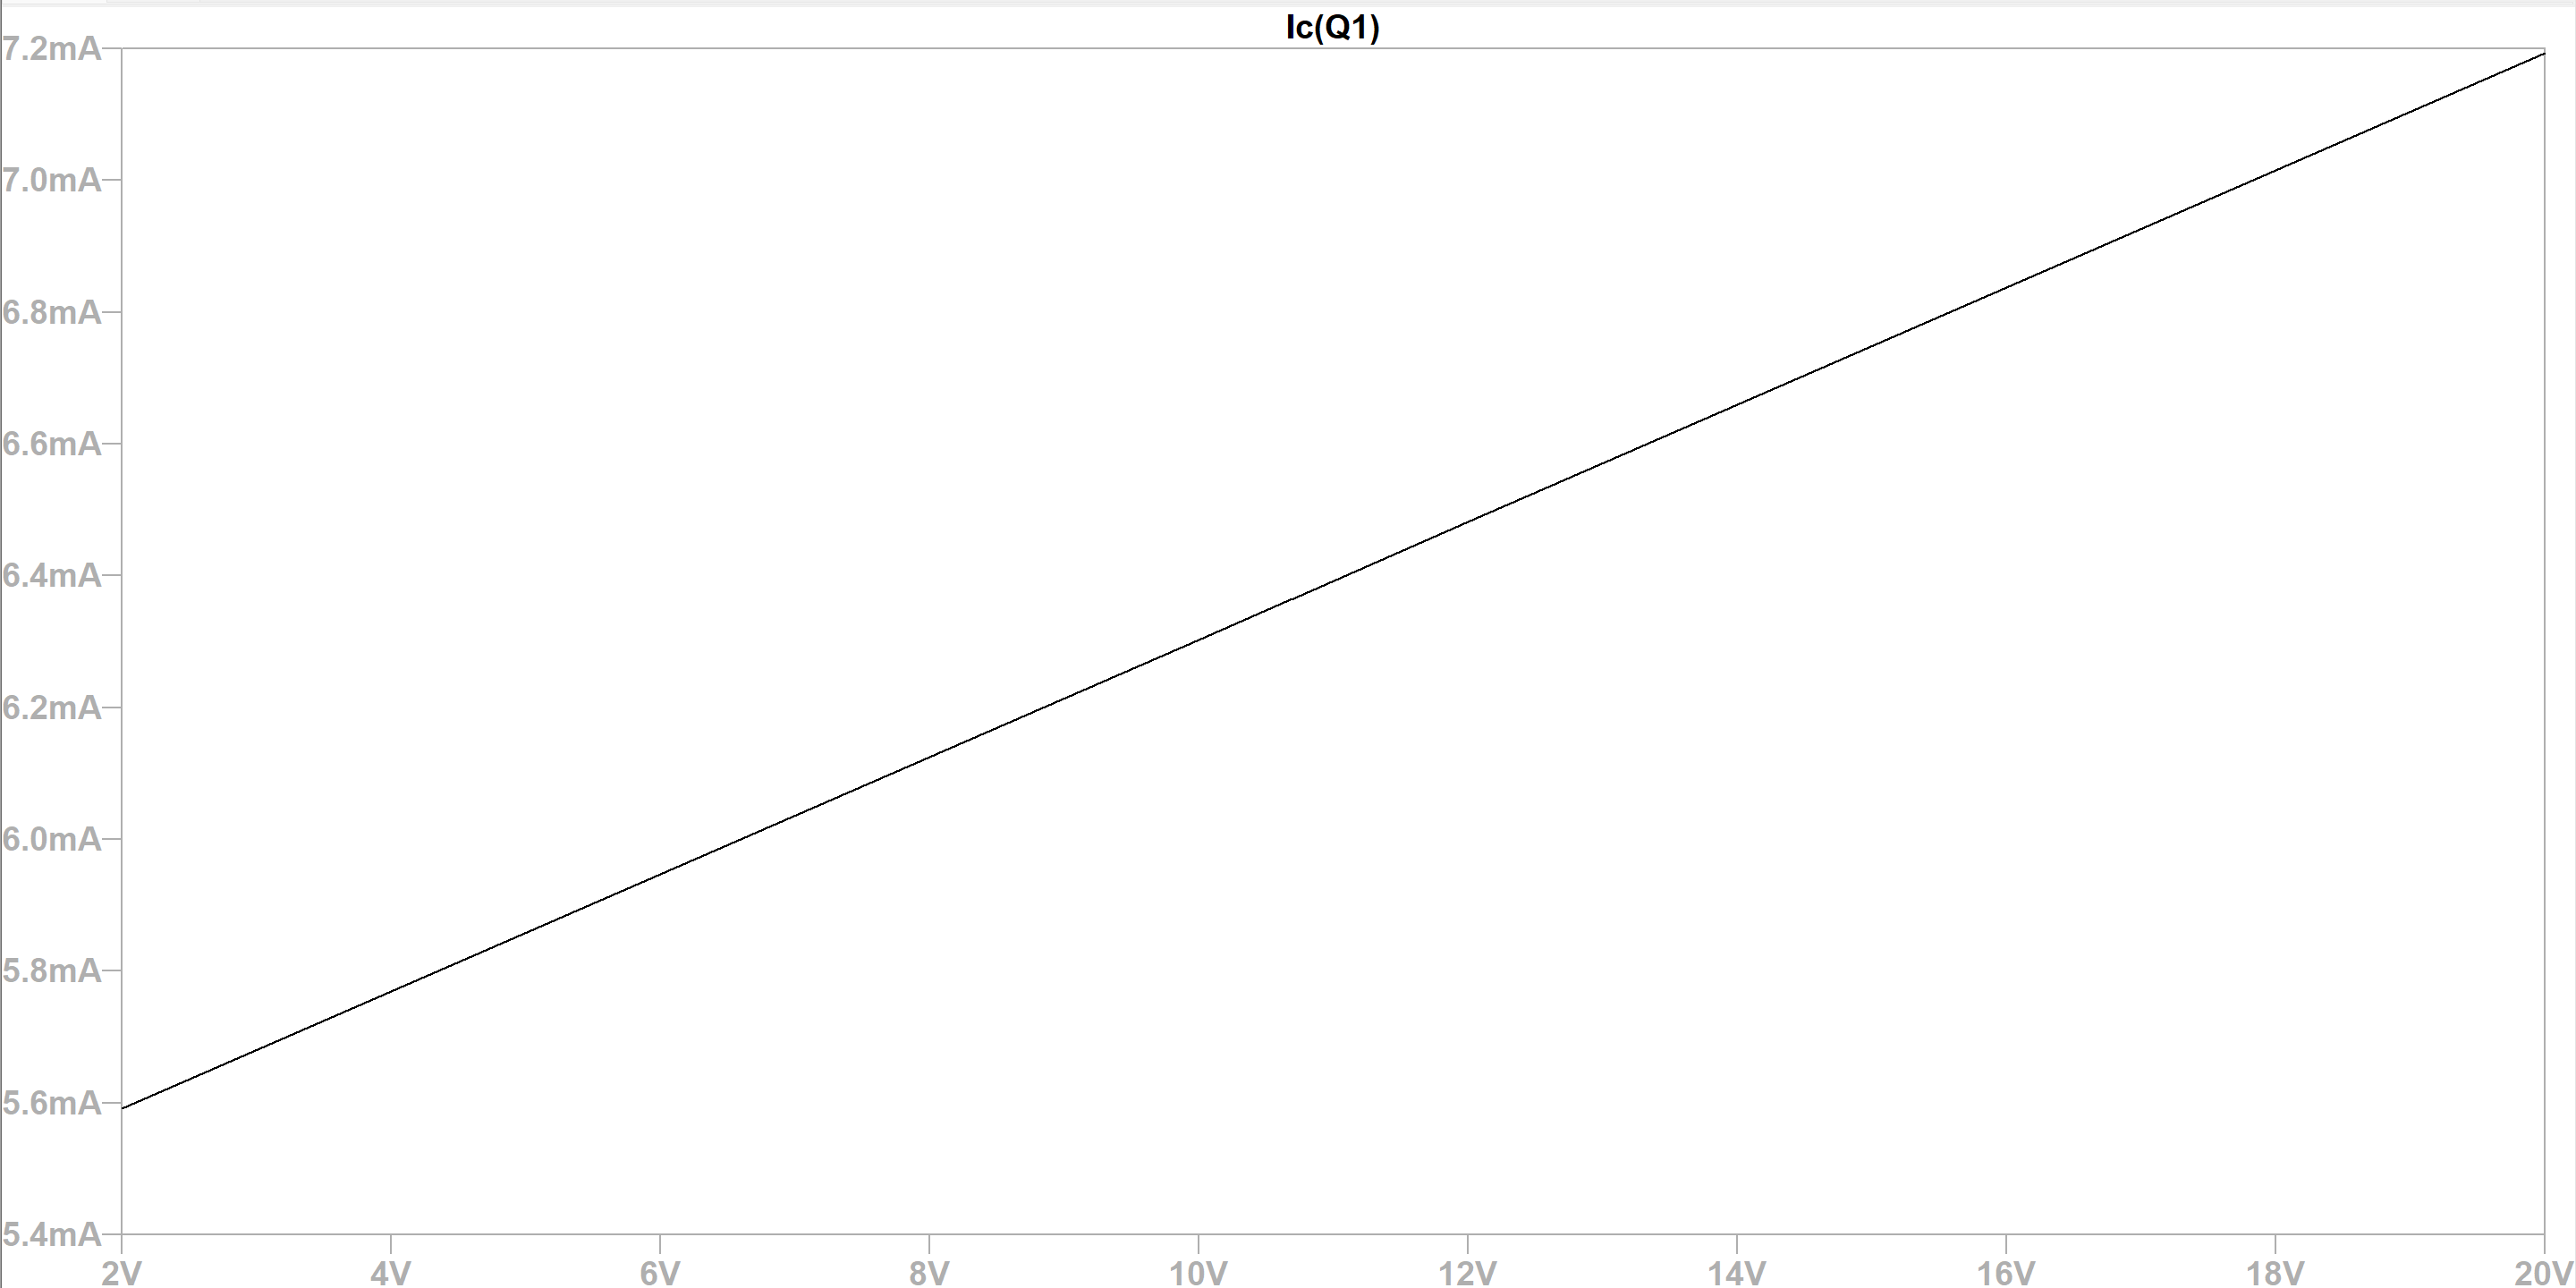
\includegraphics[width=\textwidth]{../CE-Configuration/output/output_2-20_IB=20u.png}
        \caption{$V_{CE}=2\text{--}20\text{V}$, $I_B=20\mu\text{A}$}
    \end{subfigure}
    \hfill
    \begin{subfigure}[b]{0.31\textwidth}
        \centering
        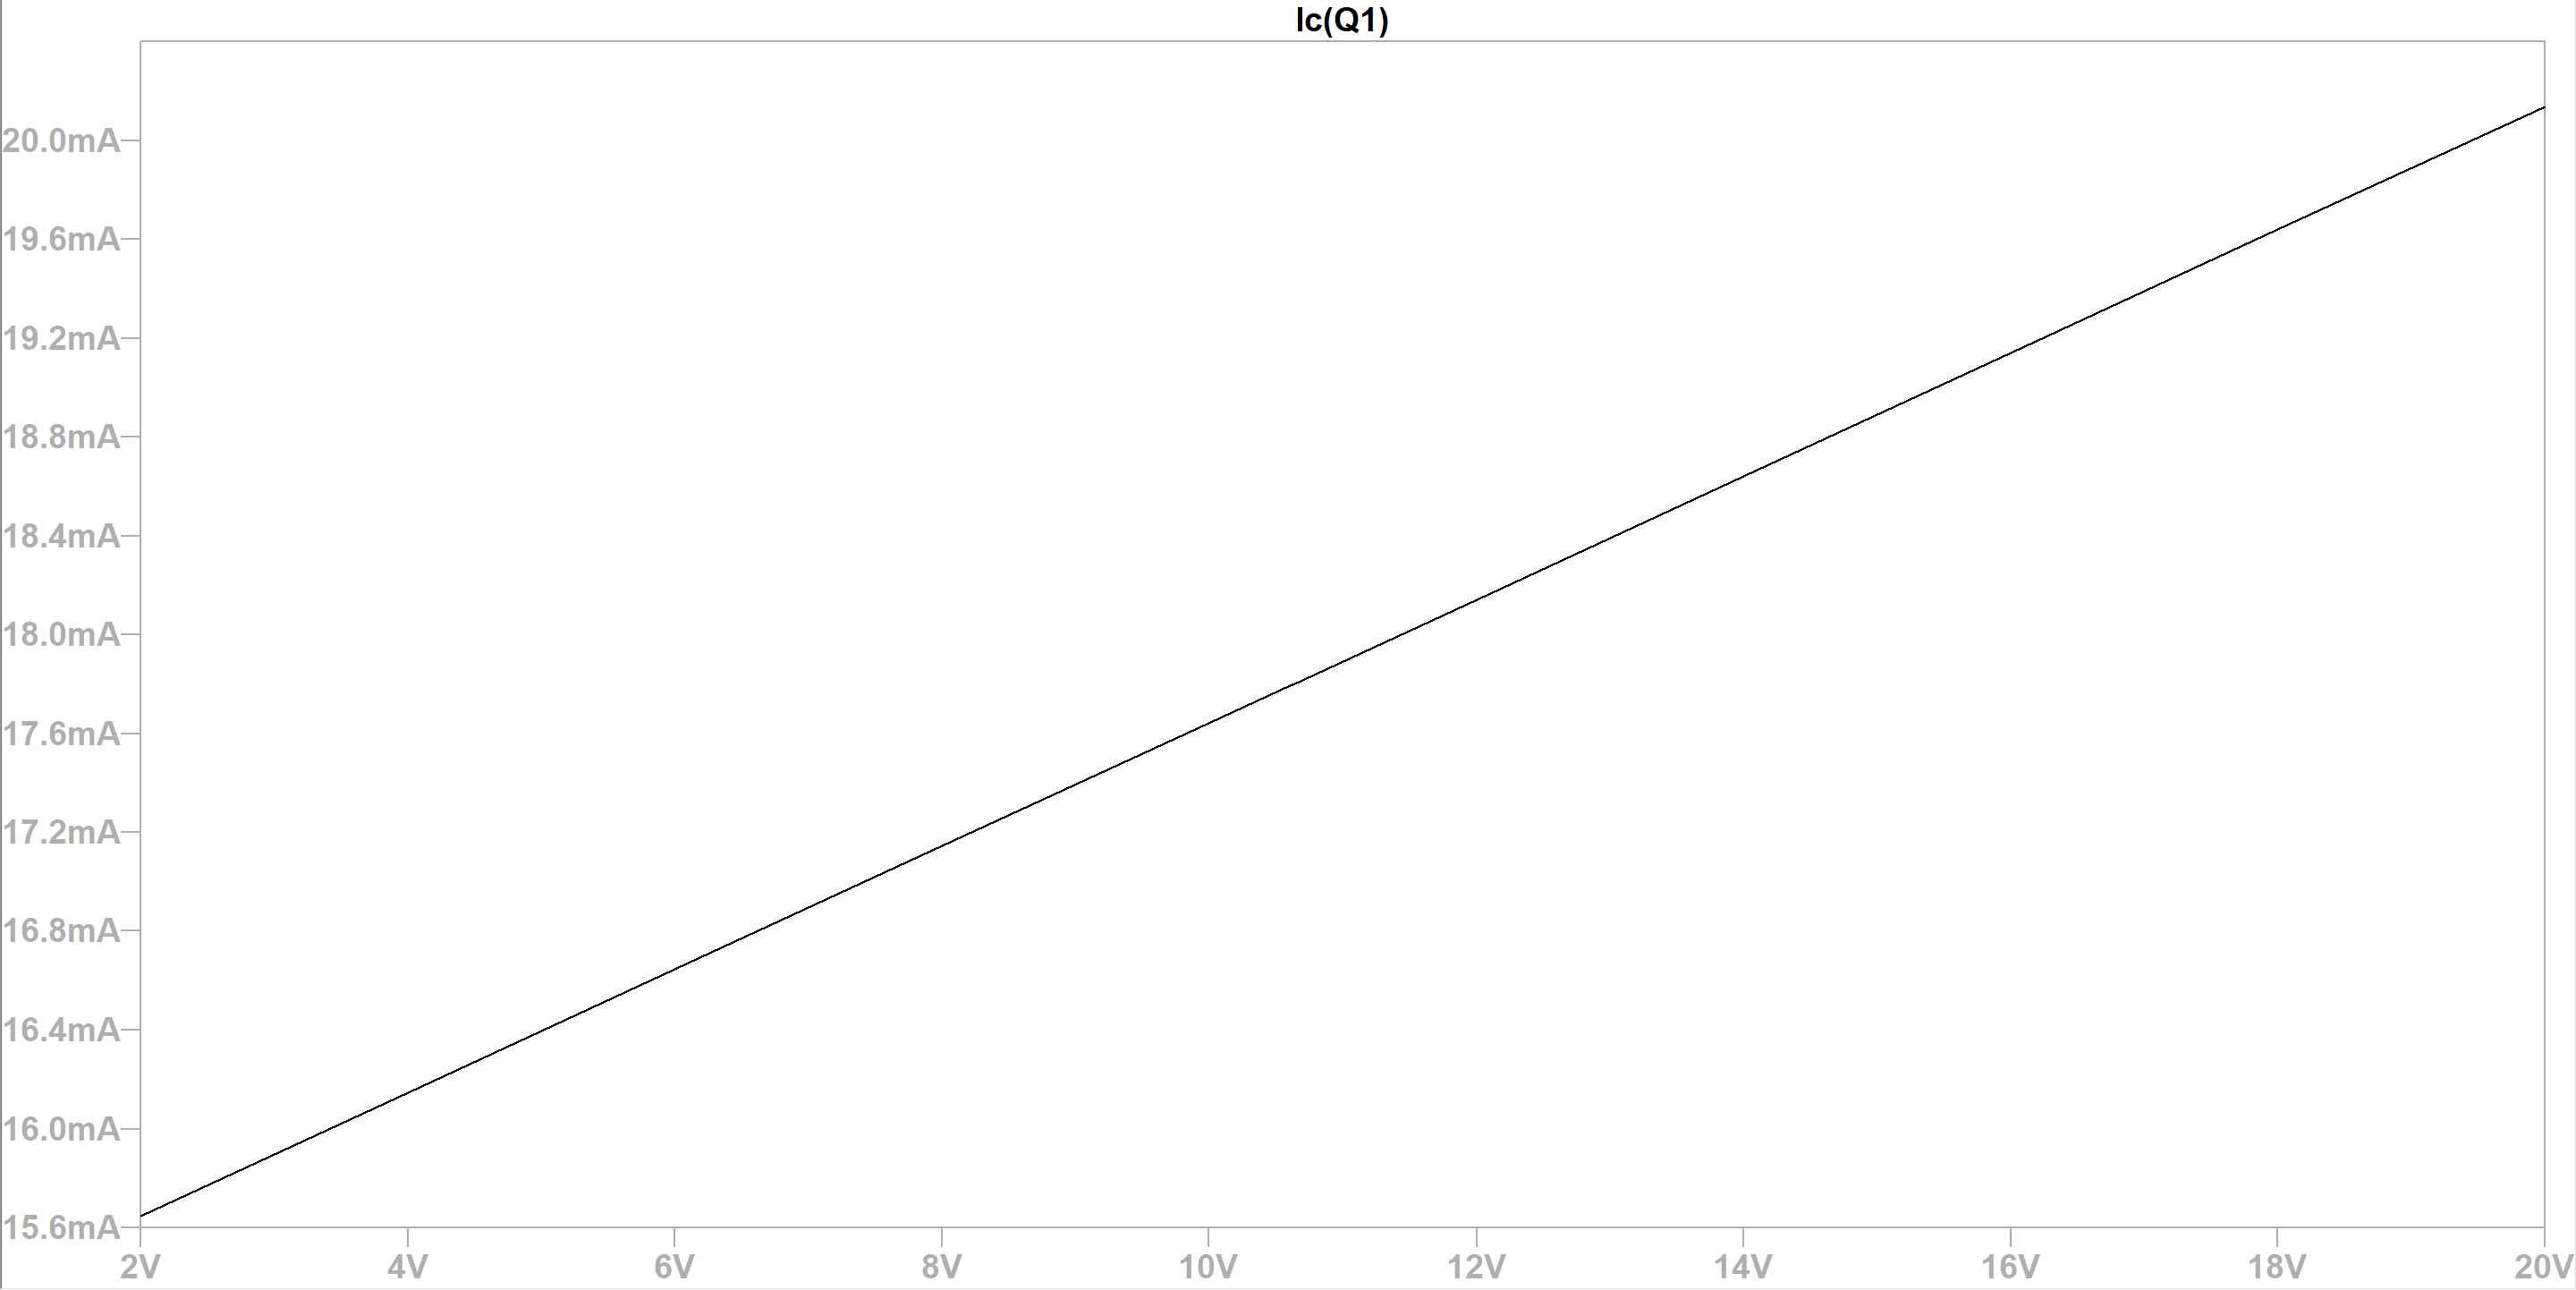
\includegraphics[width=\textwidth]{../CE-Configuration/output/output_2-20_IB=60u.png}
        \caption{$V_{CE}=2\text{--}20\text{V}$, $I_B=60\mu\text{A}$}
    \end{subfigure}
    \hfill
    \begin{subfigure}[b]{0.31\textwidth}
        \centering
        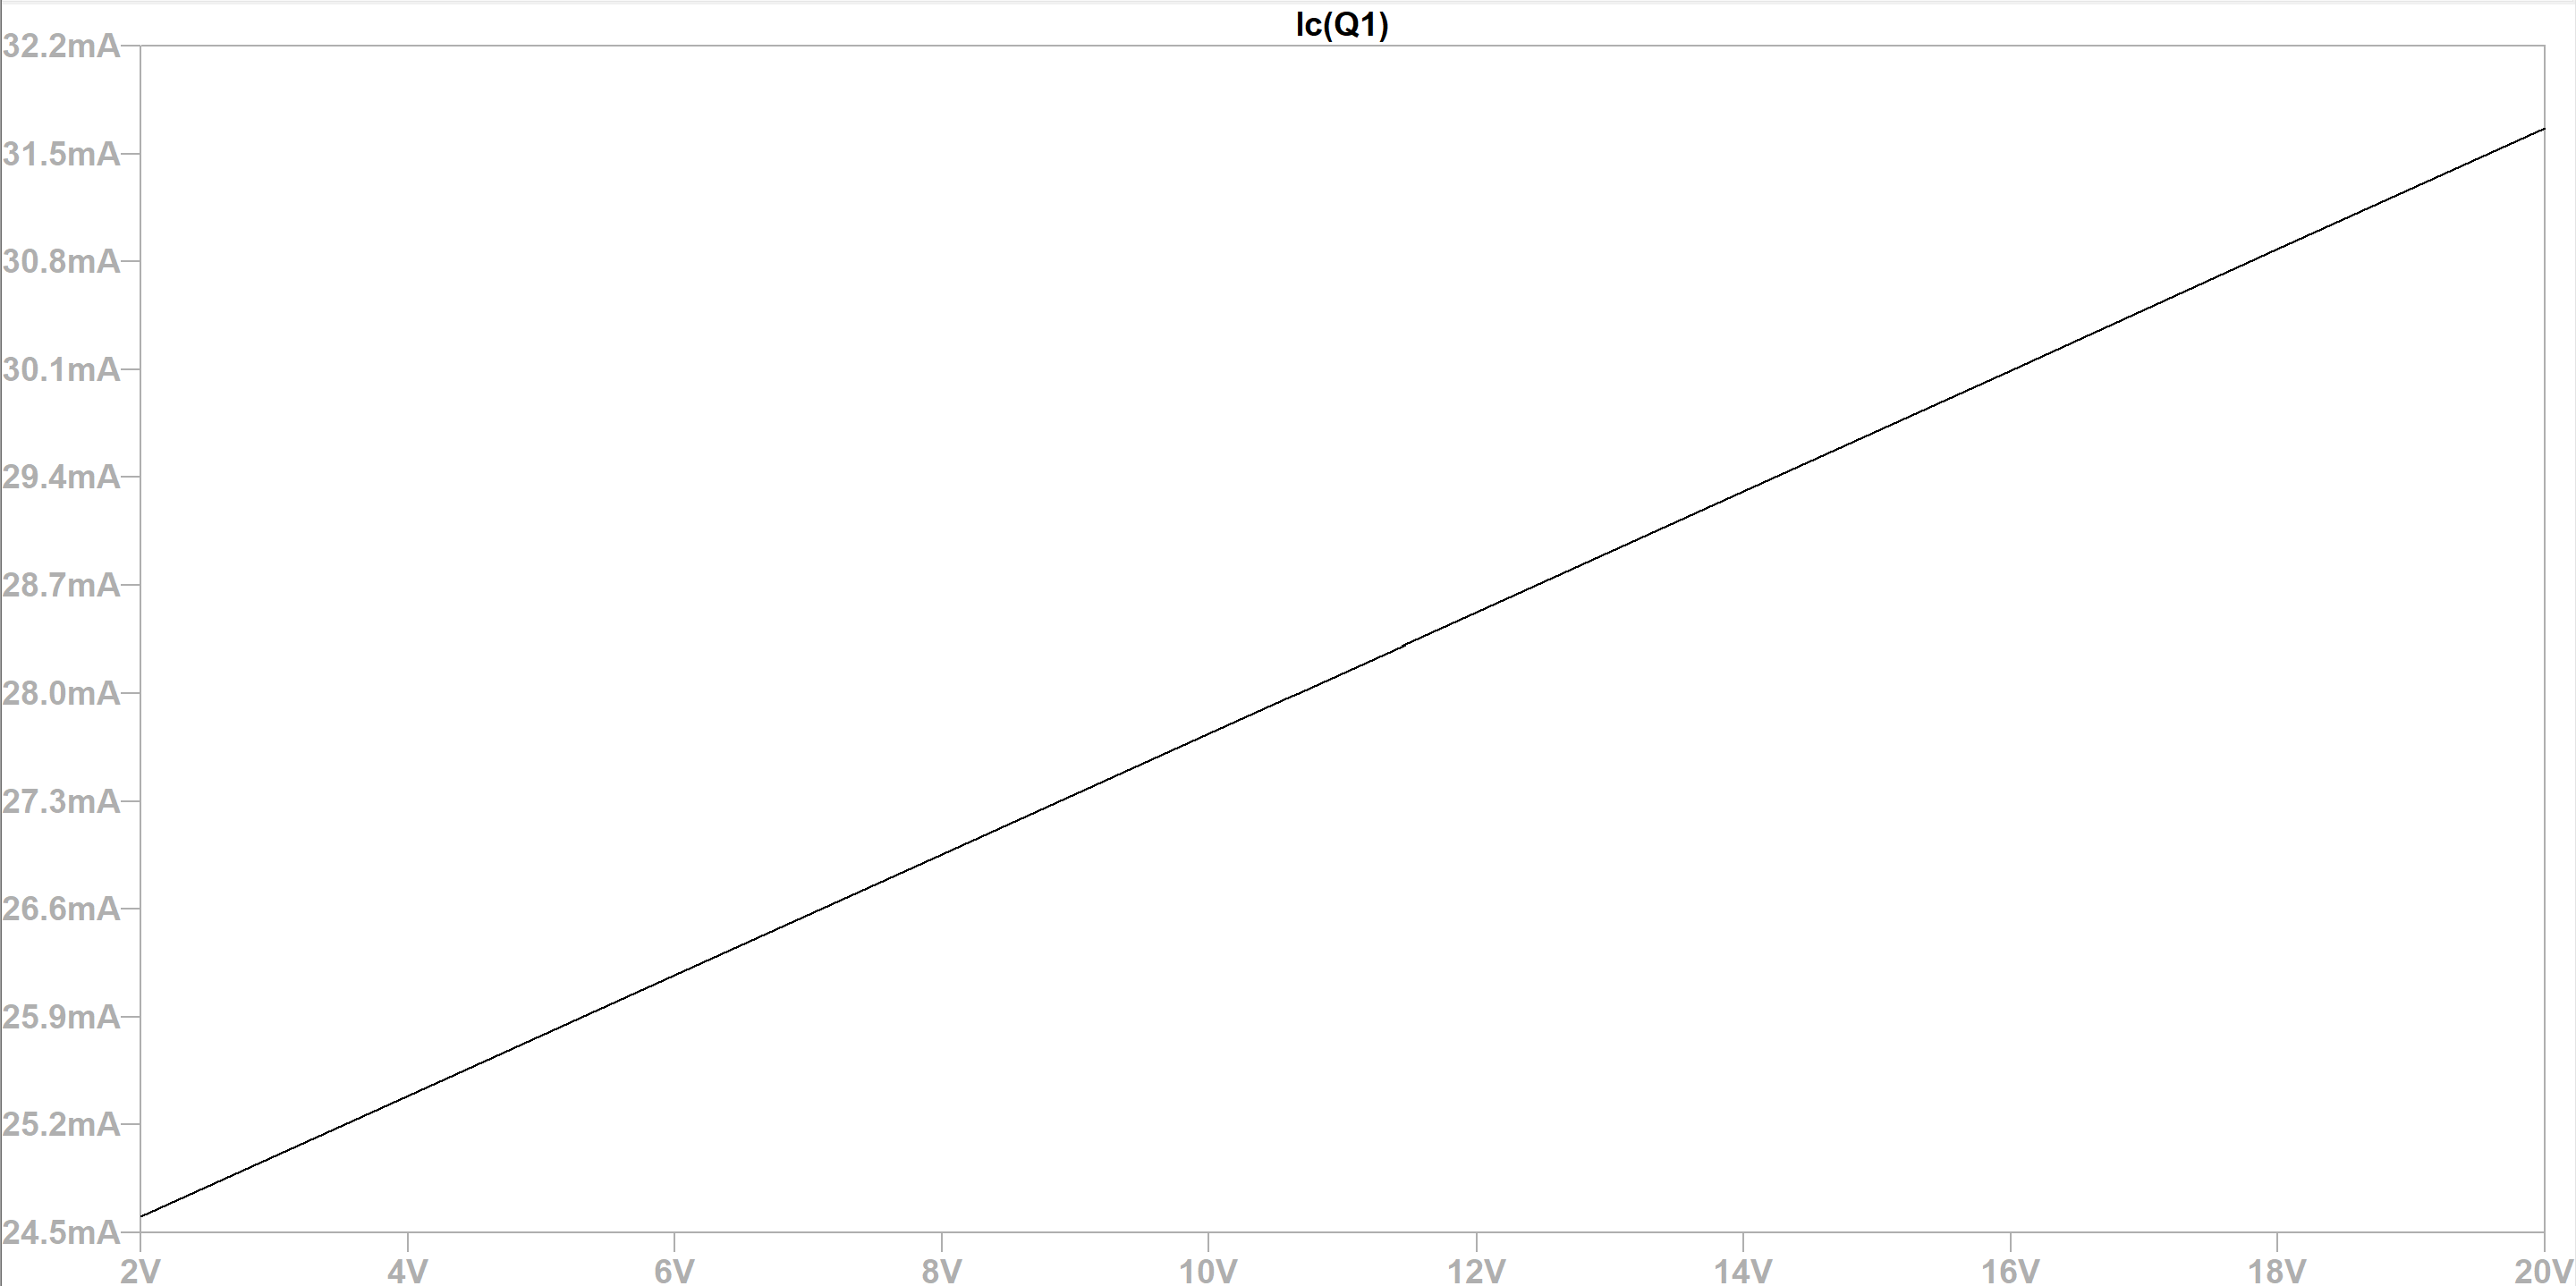
\includegraphics[width=\textwidth]{../CE-Configuration/output/output_2-20_IB=100u.png}
        \caption{$V_{CE}=2\text{--}20\text{V}$, $I_B=100\mu\text{A}$}
    \end{subfigure}
    \caption{LTspice Simulation of CE Output Characteristics ($I_C$ vs $V_{CE}$) in Saturation and Active Regions.}
    \label{fig:ce_output_sim}
\end{figure}

\subsection{Experimental Observation Tables (Hardware Data)}

\begin{table}[H]
\centering
\caption{CE Input Characteristics Observation Table ($I_B$ vs $V_{BE}$)}
\begin{tabular}{c c c c c}
\toprule
\textbf{S.No.} & \textbf{$V_{BE}$ (V)} & \textbf{$I_B$ ($\mu$A) at $V_{CE}=1$V} & \textbf{$I_B$ ($\mu$A) at $V_{CE}=5$V} & \textbf{$I_B$ ($\mu$A) at $V_{CE}=10$V} \\
\midrule
1  & 0.00 & & & \\
2  & 0.10 & & & \\
3  & 0.20 & & & \\
4  & 0.30 & & & \\
5  & 0.40 & & & \\
6  & 0.50 & & & \\
7  & 0.55 & & & \\
8  & 0.60 & & & \\
9  & 0.62 & & & \\
10 & 0.64 & & & \\
11 & 0.66 & & & \\
12 & 0.68 & & & \\
13 & 0.70 & & & \\
\bottomrule
\end{tabular}
\end{table}

\begin{table}[H]
\centering
\caption{CE Output Characteristics Observation Table ($I_C$ vs $V_{CE}$)}
\begin{tabular}{c c c c c}
\toprule
\textbf{S.No.} & \textbf{$V_{CE}$ (V)} & \textbf{$I_C$ (mA) at $I_B=20\ \mu$A} & \textbf{$I_C$ (mA) at $I_B=60\ \mu$A} & \textbf{$I_C$ (mA) at $I_B=100\ \mu$A} \\
\midrule
1  & 0.0 & & & \\
2  & 0.5 & & & \\
3  & 1.0 & & & \\
4  & 1.5 & & & \\
5  & 2.0 & & & \\
6  & 4.0 & & & \\
7  & 6.0 & & & \\
8  & 8.0 & & & \\
9  & 10.0 & & & \\
10 & 15.0 & & & \\
11 & 20.0 & & & \\
\bottomrule
\end{tabular}
\end{table}

\clearpage

\section{Part C \& D: Common Base (CB) Configuration}

\subsection{Theoretical Background}
In the Common Base (CB) configuration, the base terminal is grounded and common to both input (emitter-base) and output (collector-base) circuits.
\begin{itemize}
    \item \textbf{Input Characteristics:} Plot of Emitter Current ($I_E$) vs Emitter-Base Voltage ($V_{EB}$) at constant $V_{CB}$. $J_{EB}$ is forward-biased, yielding a very sharp exponential diode curve. Increasing $V_{CB}$ accelerates minority carrier extraction across the base, slightly increasing $I_E$ for a given $V_{EB}$.
    \item \textbf{Output Characteristics:} Plot of Collector Current ($I_C$) vs $V_{CB}$ at constant $I_E$. Once $V_{CB} > 0\text{ V}$, $I_C \approx \alpha I_E$. The curves are almost perfectly flat, indicating extremely high output resistance.
    \item \textbf{Key Parameters:}
    \begin{align}
        \text{Input Resistance: } r_i &= \left. \frac{\Delta V_{EB}}{\Delta I_E} \right|_{V_{CB} = \text{const}} \quad (\text{Very Low: }\approx 10\text{--}50\ \Omega) \\
        \text{Output Resistance: } r_o &= \left. \frac{\Delta V_{CB}}{\Delta I_C} \right|_{I_E = \text{const}} \quad (\text{Very High: }\approx 1\text{ M}\Omega) \\
        \text{Current Gain: } \alpha &= \left. \frac{\Delta I_C}{\Delta I_E} \right|_{V_{CB} = \text{const}} \quad (< 1\text{, typically } 0.95\text{--}0.99)
    \end{align}
\end{itemize}

\subsection{Circuit Schematic and Simulation Waveforms}
\begin{figure}[H]
    \centering
    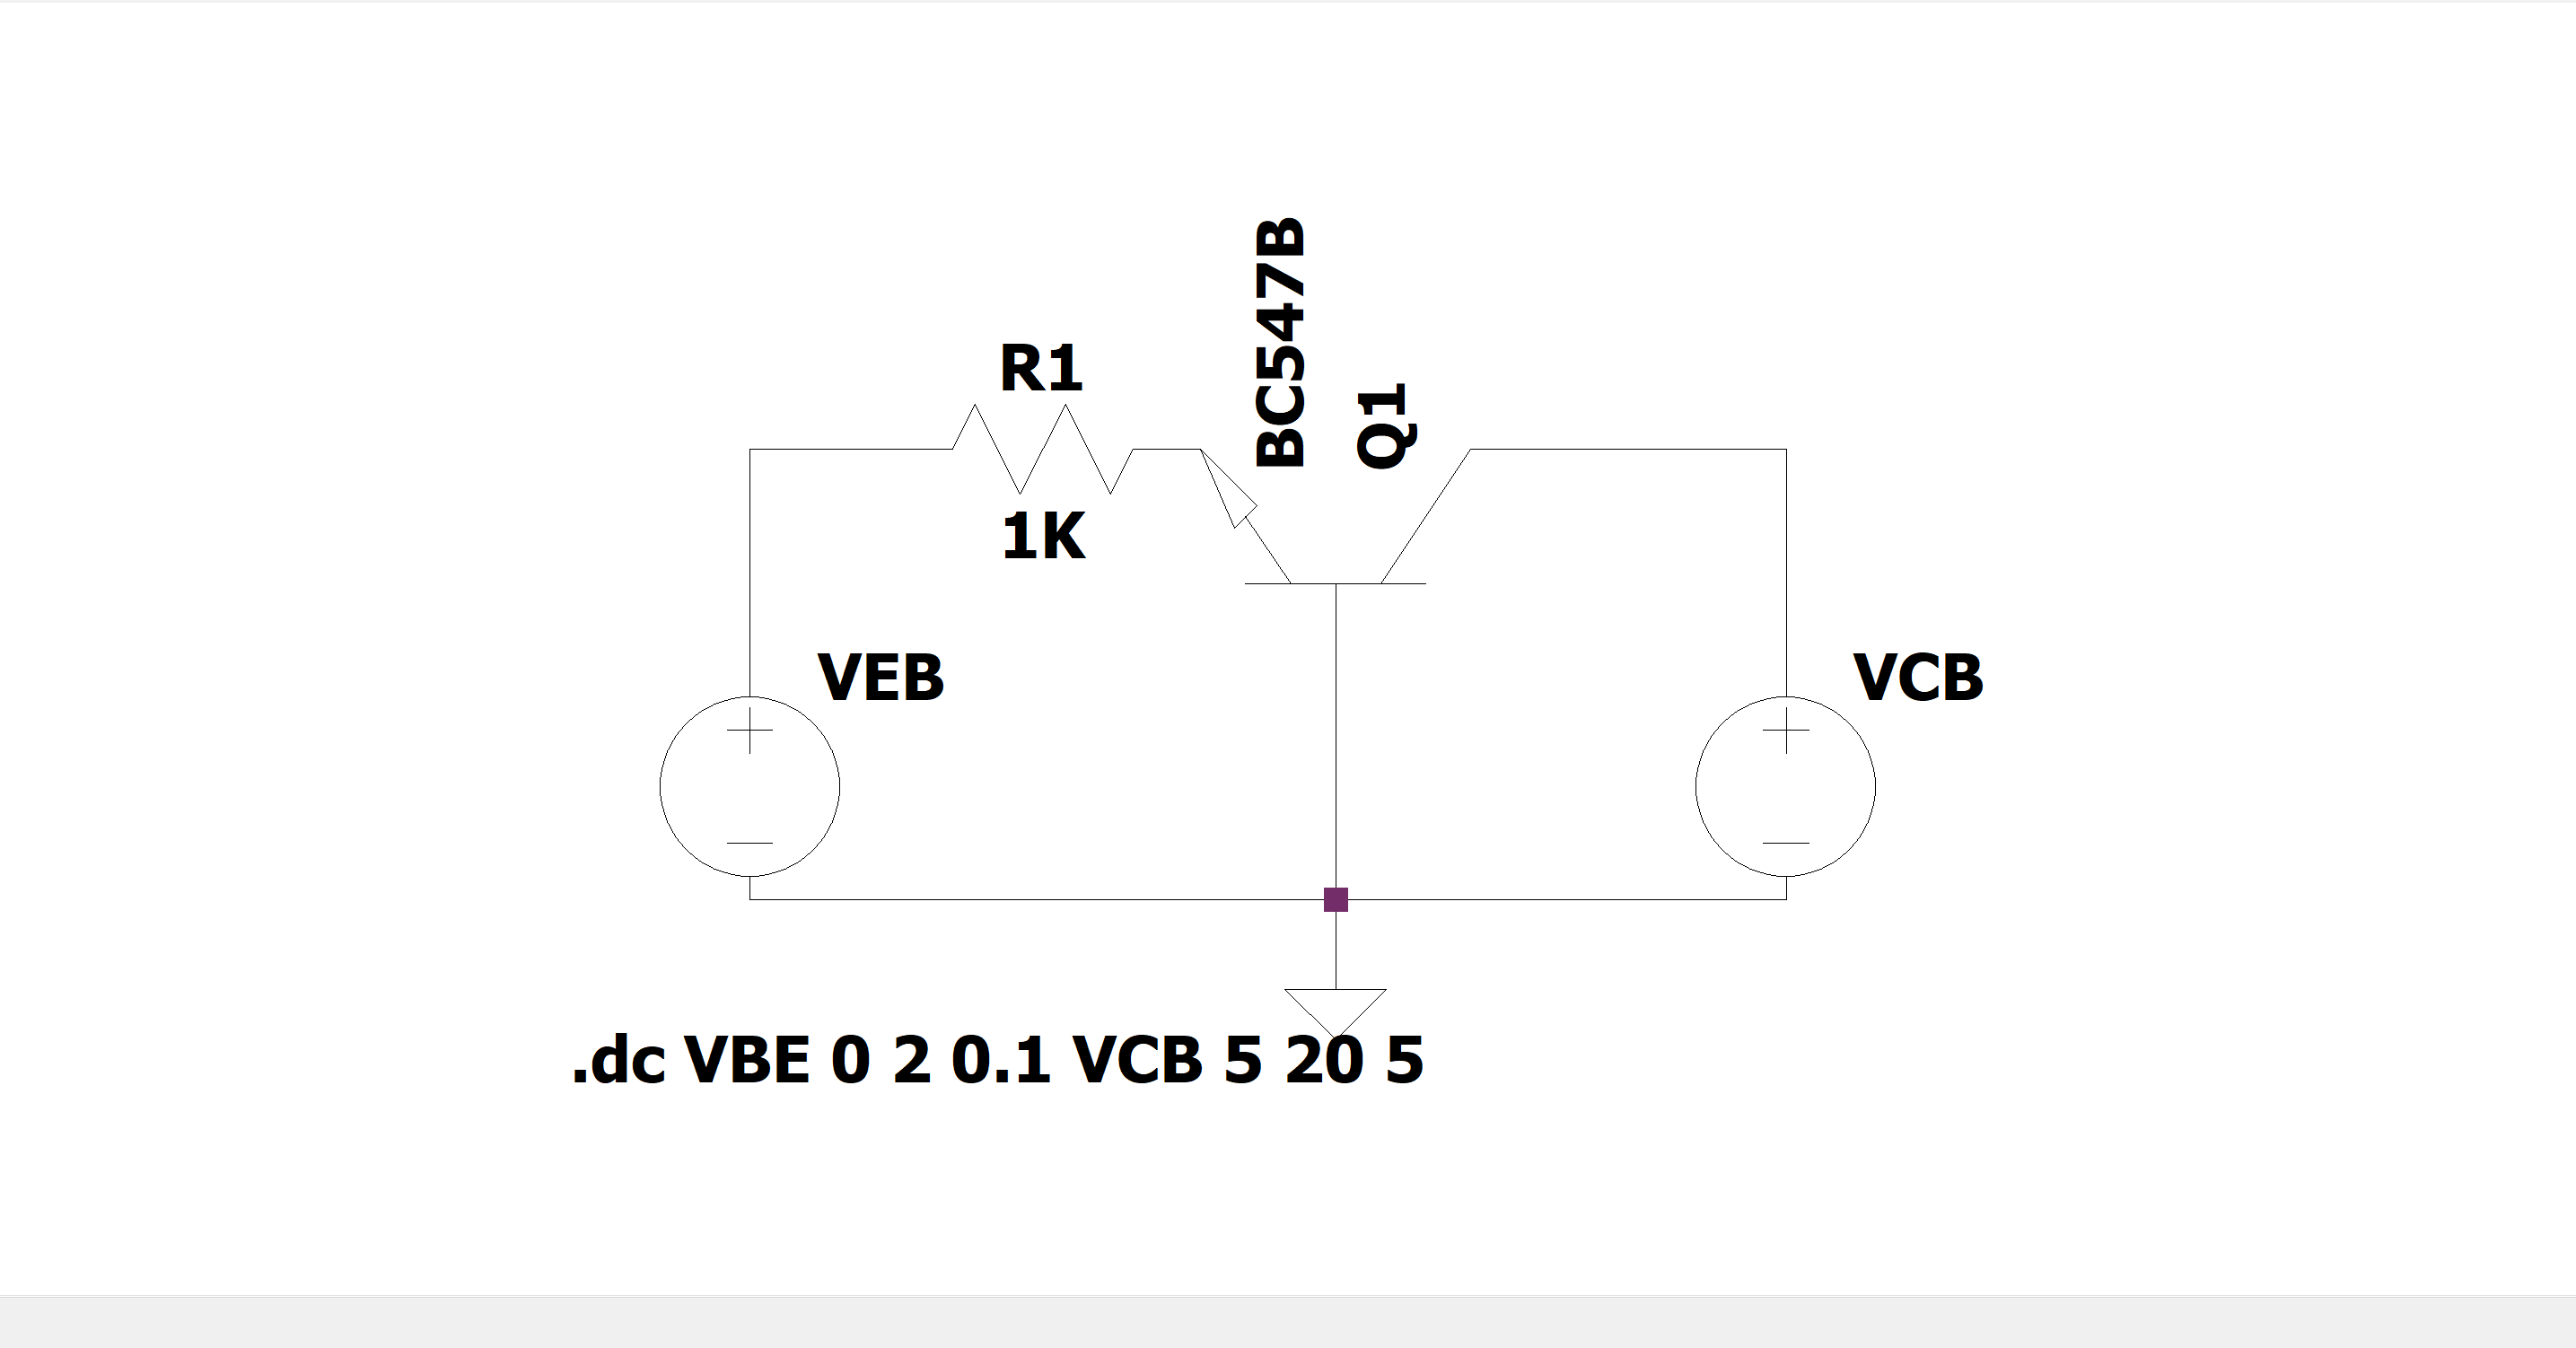
\includegraphics[width=0.55\textwidth]{../CB-Configuration/Schematic.png}
    \caption{LTspice Circuit Schematic for Common Base (CB) Configuration.}
    \label{fig:cb_schematic}
\end{figure}

\subsubsection{CB Input Characteristics Simulation}
\begin{figure}[H]
    \centering
    \begin{subfigure}[b]{0.45\textwidth}
        \centering
        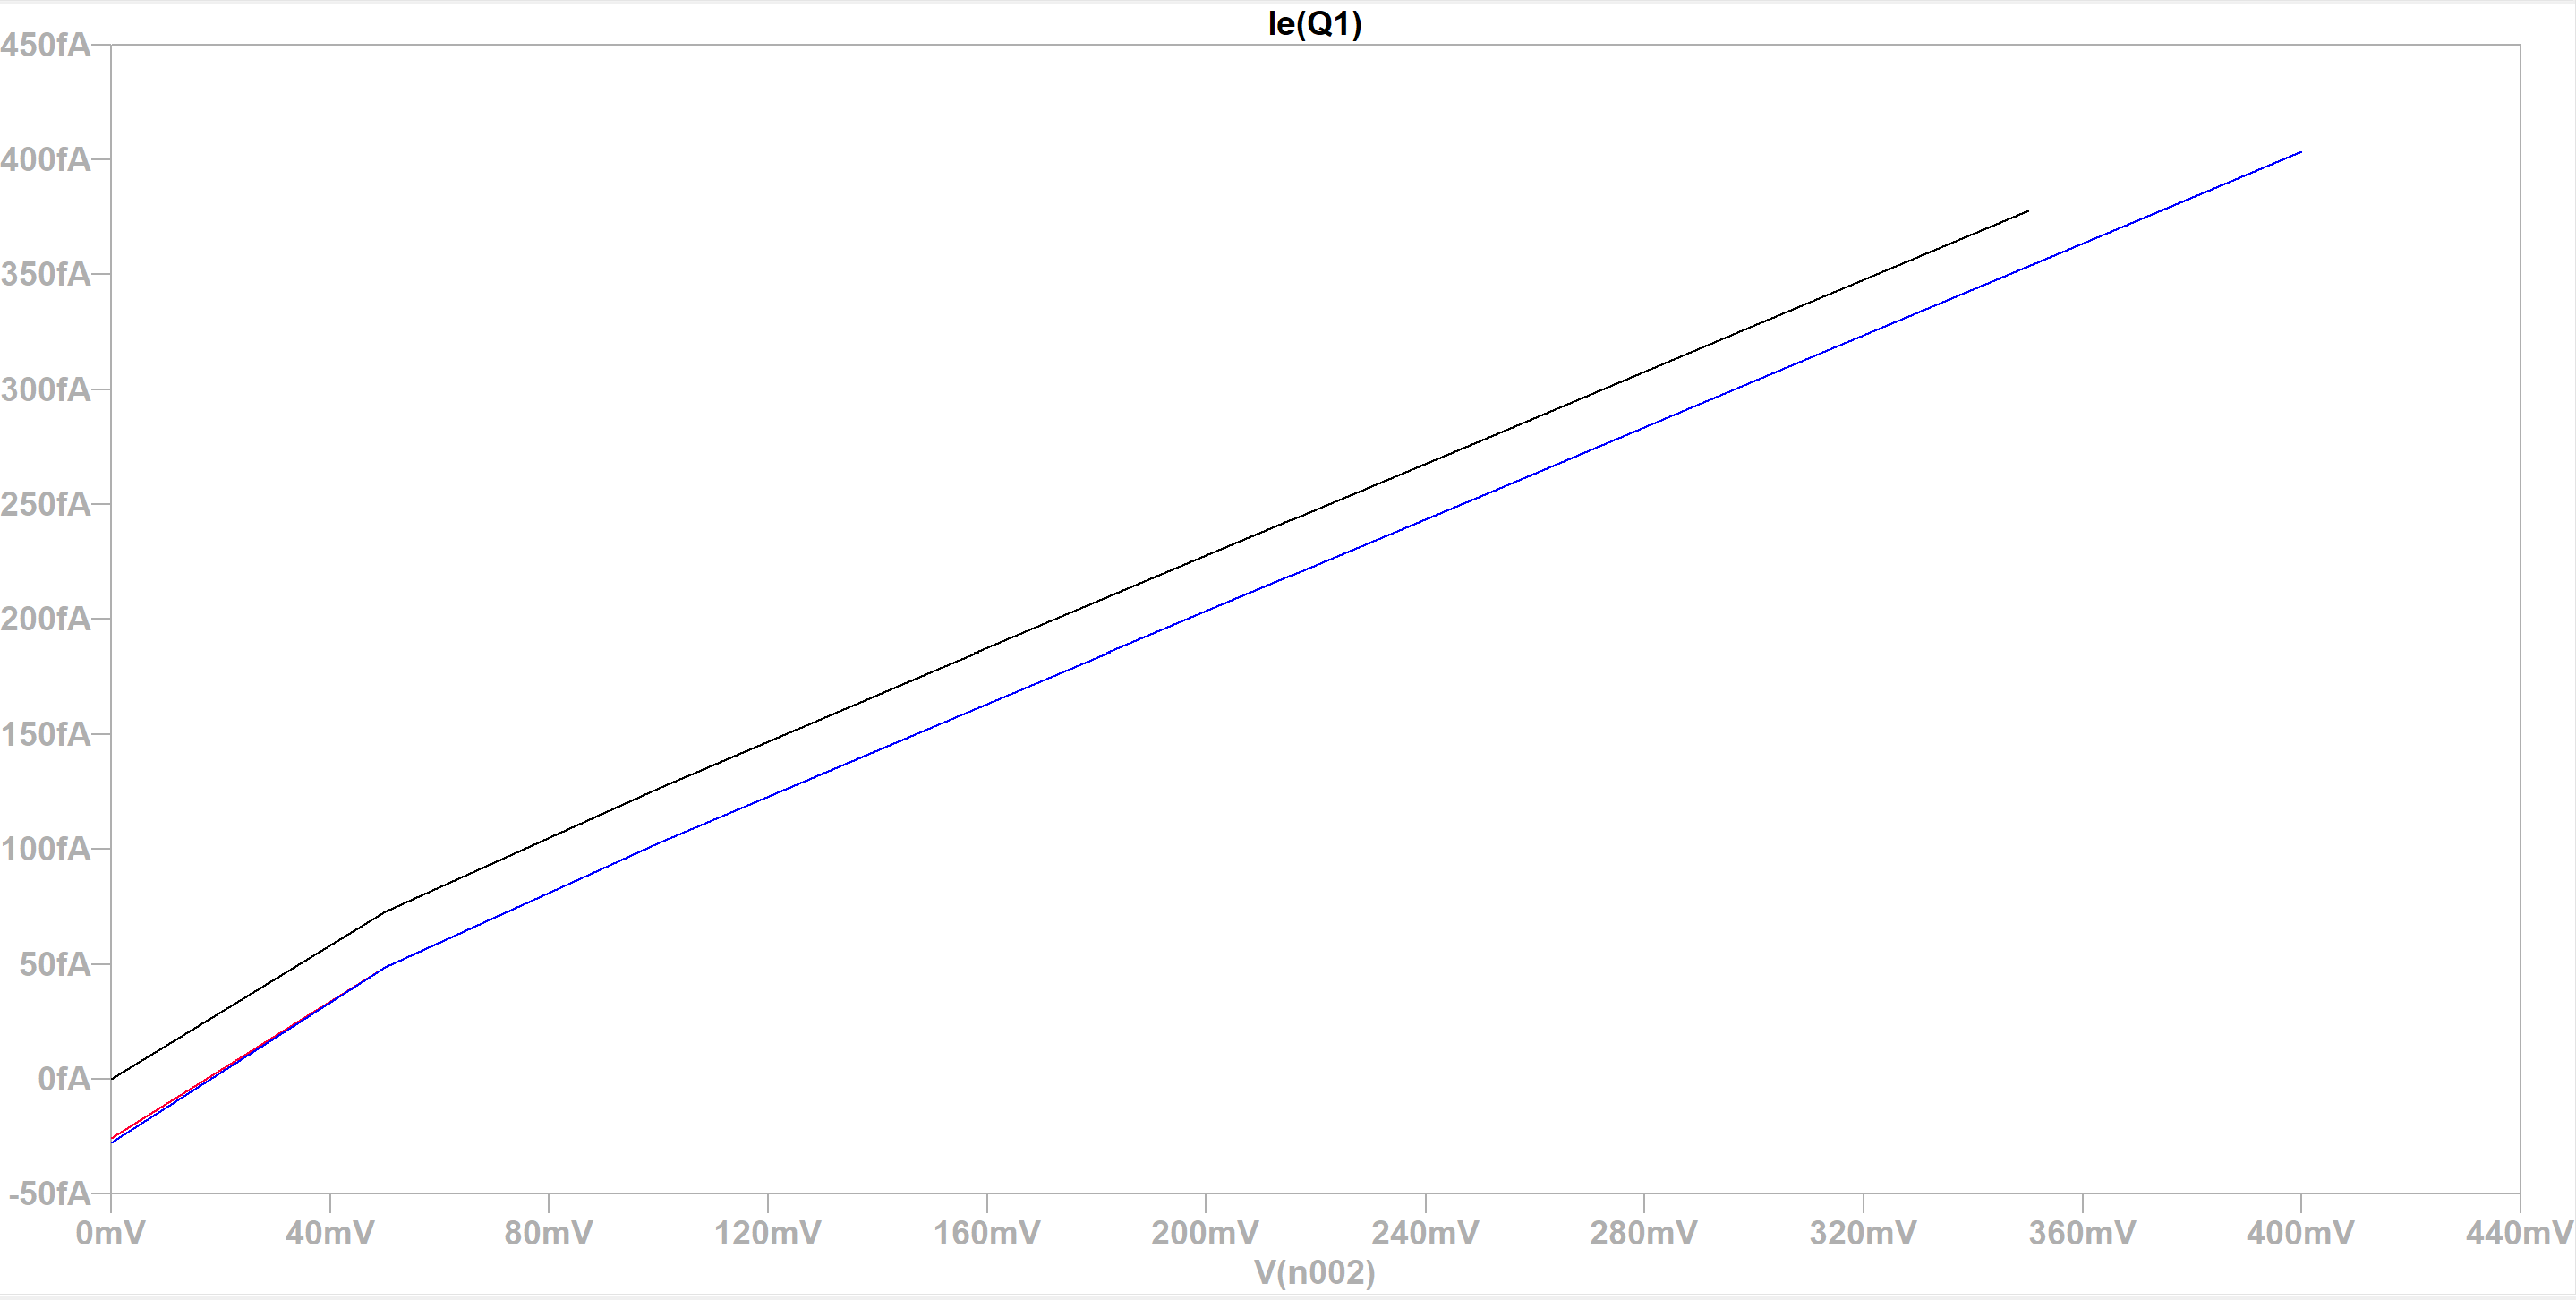
\includegraphics[width=\textwidth]{../CB-Configuration/input/input_0-0.4.png}
        \caption{Low Voltage Range ($V_{EB} = 0\text{--}0.4\text{ V}$)}
    \end{subfigure}
    \hfill
    \begin{subfigure}[b]{0.45\textwidth}
        \centering
        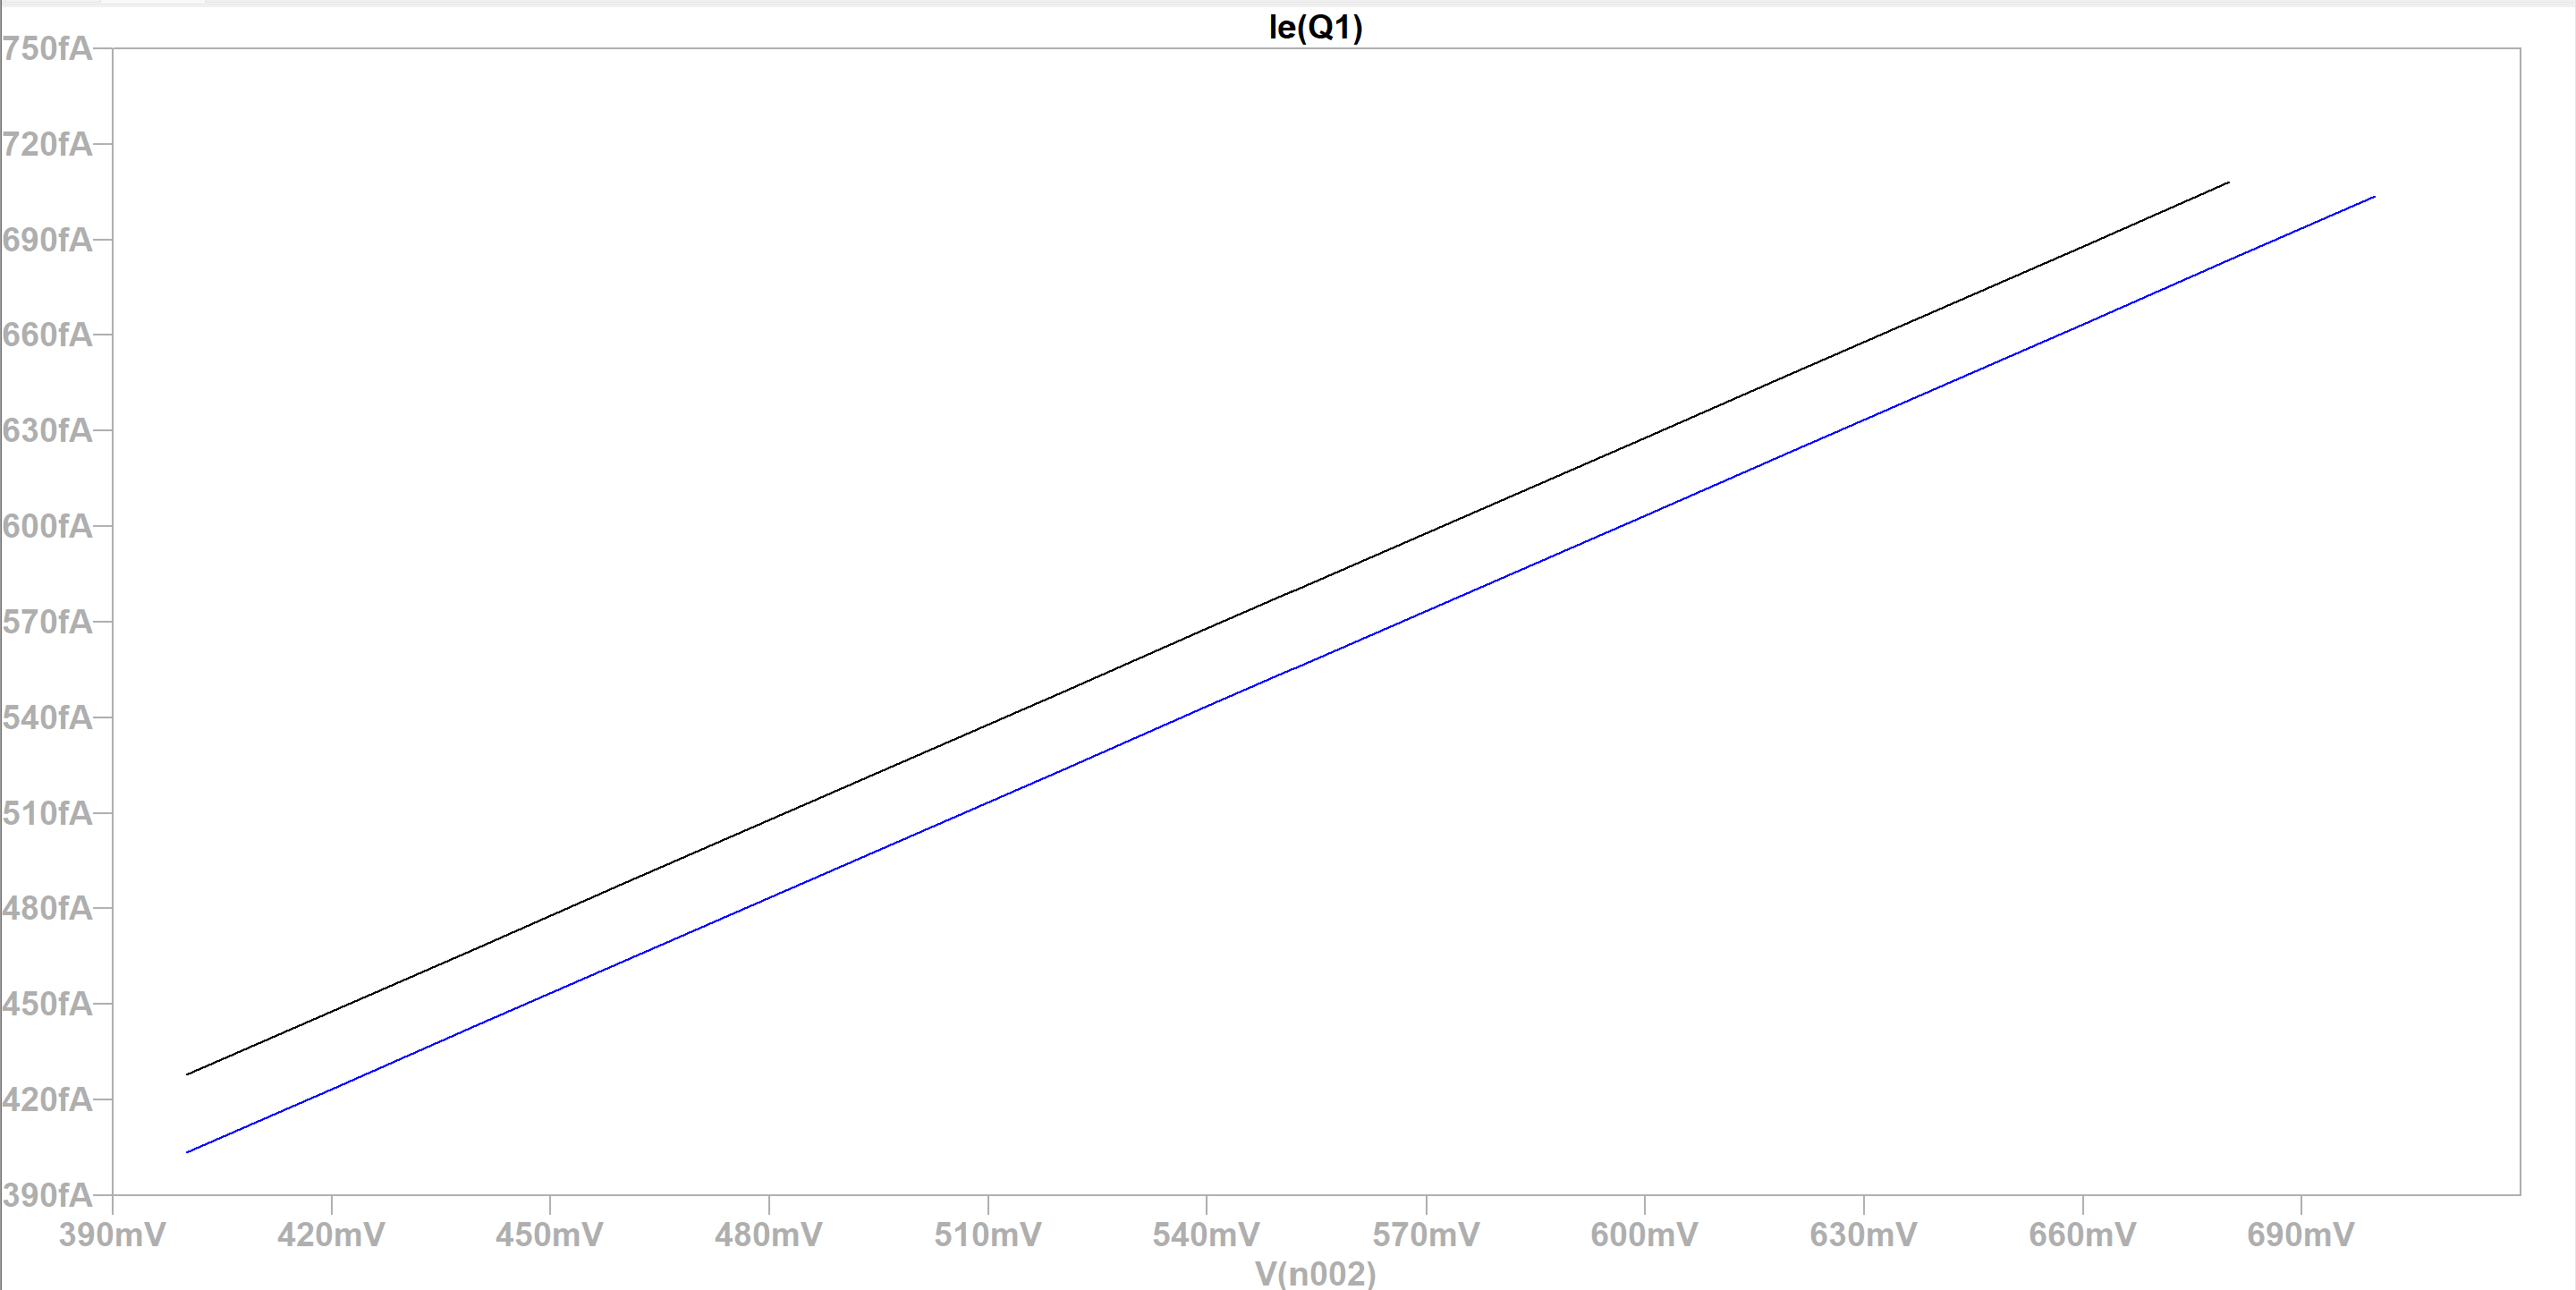
\includegraphics[width=\textwidth]{../CB-Configuration/input/input_0.4-0.7.png}
        \caption{Conduction Range ($V_{EB} = 0.4\text{--}0.7\text{ V}$)}
    \end{subfigure}
    \caption{LTspice Simulation of CB Input Characteristics ($I_E$ vs $V_{EB}$) for various $V_{CB}$ values.}
    \label{fig:cb_input_sim}
\end{figure}

\subsubsection{CB Output Characteristics Simulation}
\begin{figure}[H]
    \centering
    \begin{subfigure}[b]{0.45\textwidth}
        \centering
        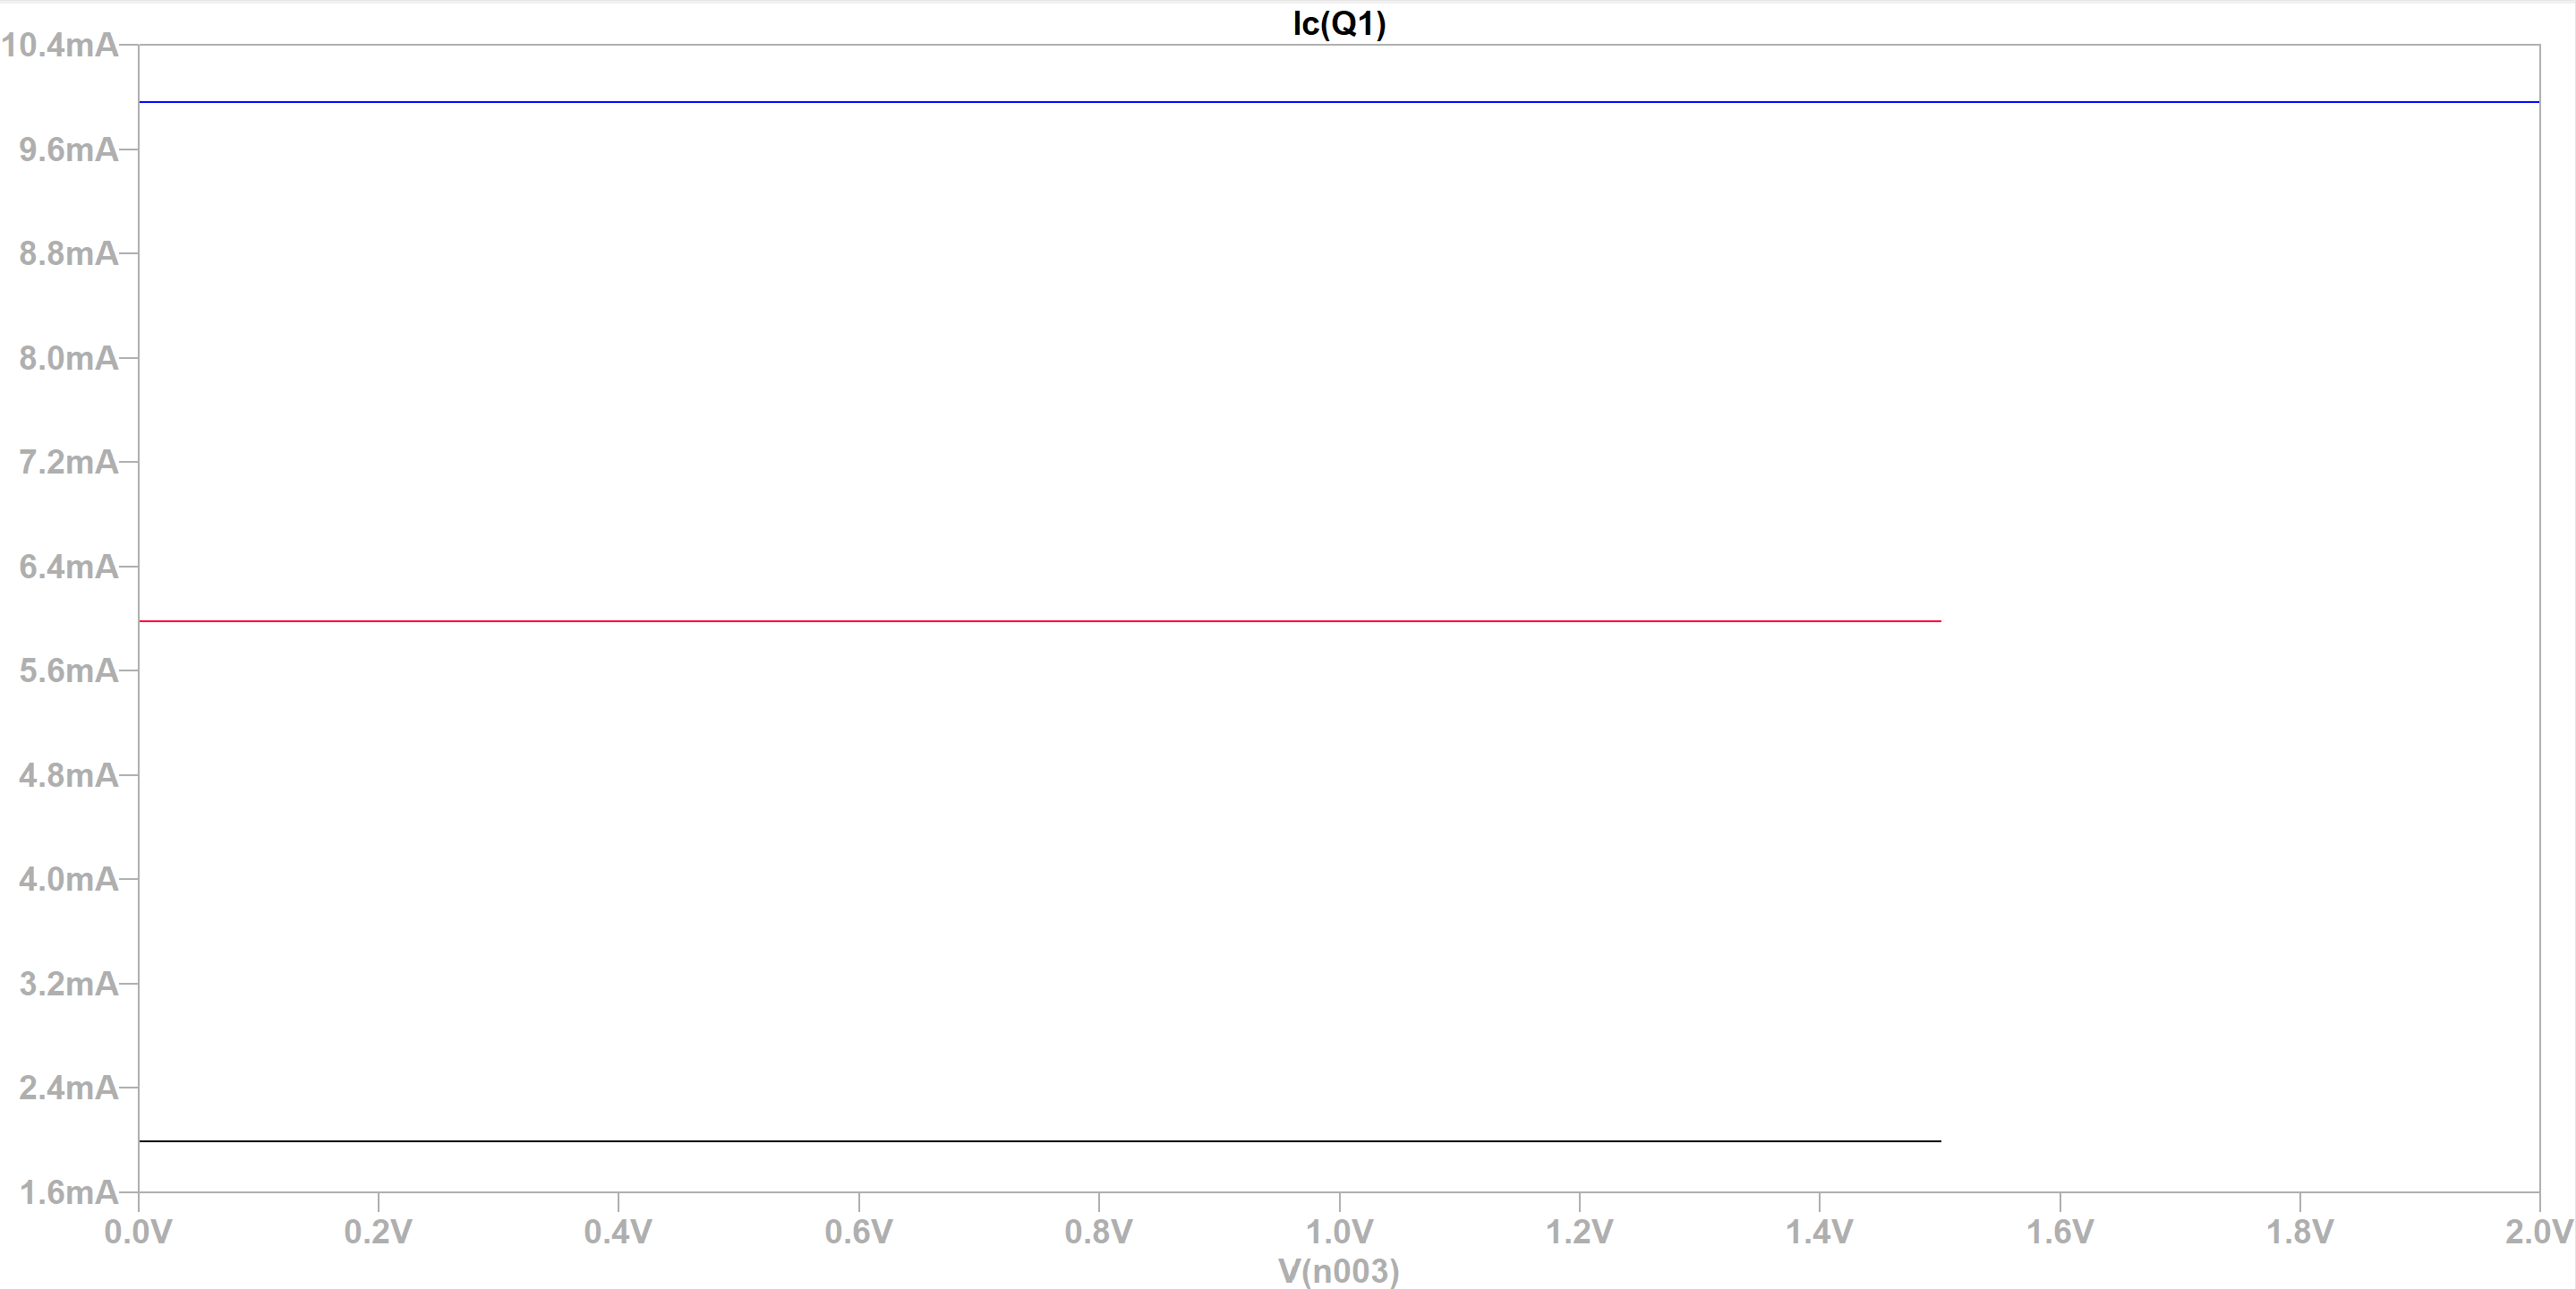
\includegraphics[width=\textwidth]{../CB-Configuration/output/output_0-2.png}
        \caption{Knee / Transition Region ($V_{CB} = 0\text{--}2\text{ V}$)}
    \end{subfigure}
    \hfill
    \begin{subfigure}[b]{0.45\textwidth}
        \centering
        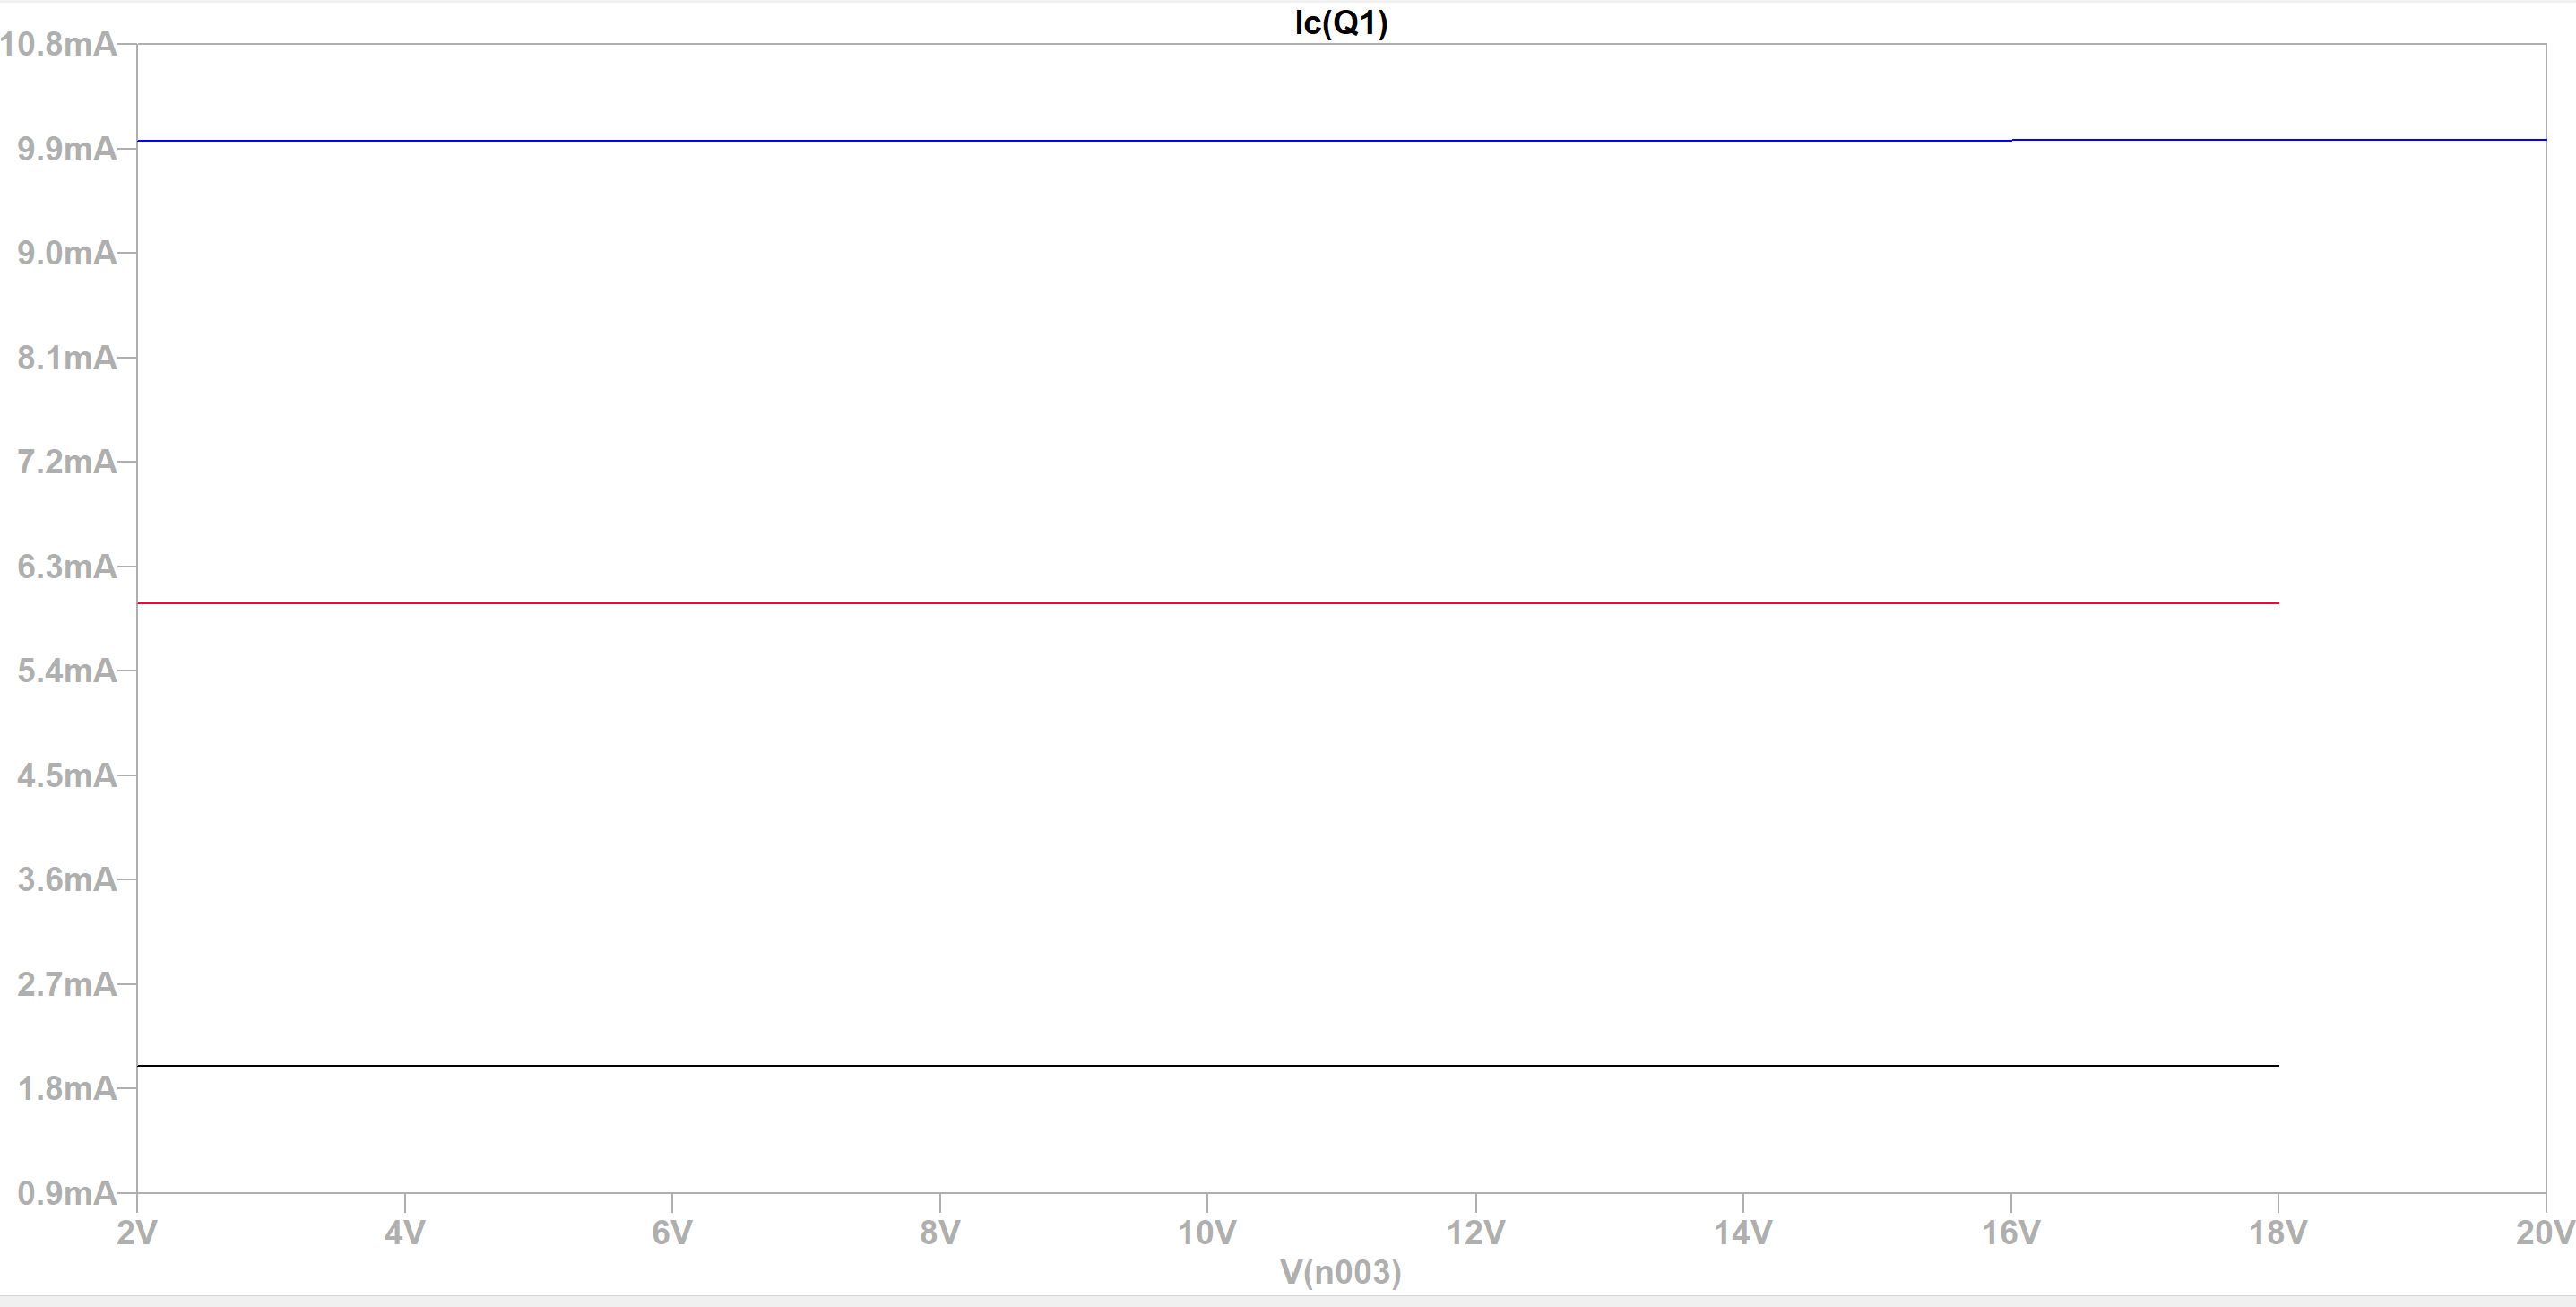
\includegraphics[width=\textwidth]{../CB-Configuration/output/output_2-20.png}
        \caption{Active Region ($V_{CB} = 2\text{--}20\text{ V}$)}
    \end{subfigure}
    \caption{LTspice Simulation of CB Output Characteristics ($I_C$ vs $V_{CB}$) for $I_E = 2\text{ mA}, 6\text{ mA}, 10\text{ mA}$.}
    \label{fig:cb_output_sim}
\end{figure}

\subsection{Experimental Observation Tables (Hardware Data)}

\begin{table}[H]
\centering
\caption{CB Input Characteristics Observation Table ($I_E$ vs $V_{EB}$)}
\begin{tabular}{c c c c c}
\toprule
\textbf{S.No.} & \textbf{$V_{EB}$ (V)} & \textbf{$I_E$ (mA) at $V_{CB}=0$V} & \textbf{$I_E$ (mA) at $V_{CB}=5$V} & \textbf{$I_E$ (mA) at $V_{CB}=10$V} \\
\midrule
1  & 0.00 & & & \\
2  & 0.10 & & & \\
3  & 0.20 & & & \\
4  & 0.30 & & & \\
5  & 0.40 & & & \\
6  & 0.50 & & & \\
7  & 0.55 & & & \\
8  & 0.60 & & & \\
9  & 0.62 & & & \\
10 & 0.64 & & & \\
11 & 0.66 & & & \\
12 & 0.68 & & & \\
13 & 0.70 & & & \\
\bottomrule
\end{tabular}
\end{table}

\begin{table}[H]
\centering
\caption{CB Output Characteristics Observation Table ($I_C$ vs $V_{CB}$)}
\begin{tabular}{c c c c c}
\toprule
\textbf{S.No.} & \textbf{$V_{CB}$ (V)} & \textbf{$I_C$ (mA) at $I_E=2$mA} & \textbf{$I_C$ (mA) at $I_E=6$mA} & \textbf{$I_C$ (mA) at $I_E=10$mA} \\
\midrule
1  & 0.0 & & & \\
2  & 0.5 & & & \\
3  & 1.0 & & & \\
4  & 1.5 & & & \\
5  & 2.0 & & & \\
6  & 4.0 & & & \\
7  & 6.0 & & & \\
8  & 8.0 & & & \\
9  & 10.0 & & & \\
10 & 15.0 & & & \\
11 & 20.0 & & & \\
\bottomrule
\end{tabular}
\end{table}

\clearpage

\section{Part E \& F: Common Collector (CC) Configuration}

\subsection{Theoretical Background}
In the Common Collector (CC) configuration (Emitter Follower), the collector terminal is common to both input (base-collector) and output (emitter-collector) ports.
\begin{itemize}
    \item \textbf{Input Characteristics:} Plot of Base Current ($I_B$) vs Base-Collector Voltage ($V_{BC}$) at constant $V_{EC}$. As $V_{BC}$ increases (increasing reverse bias), $I_B$ decreases because $V_{BE} = V_{EC} - V_{BC}$ decreases for a fixed $V_{EC}$.
    \item \textbf{Output Characteristics:} Plot of Emitter Current ($I_E$) vs $V_{EC}$ at constant $I_B$. Since $I_E = (\beta + 1) I_B \approx I_C$, the curves closely mirror the CE output characteristics.
    \item \textbf{Key Parameters:}
    \begin{align}
        \text{Input Resistance: } r_i &= \left. \frac{\Delta V_{BC}}{\Delta I_B} \right|_{V_{EC} = \text{const}} \quad (\text{Very High: }\approx 100\text{ k}\Omega\text{ -- }500\text{ k}\Omega) \\
        \text{Output Resistance: } r_o &= \left. \frac{\Delta V_{EC}}{\Delta I_E} \right|_{I_B = \text{const}} \quad (\text{Very Low: }\approx 20\text{--}100\ \Omega) \\
        \text{Current Gain: } \gamma &= \left. \frac{\Delta I_E}{\Delta I_B} \right|_{V_{EC} = \text{const}} \quad (= \beta + 1 \approx 50\text{--}300)
    \end{align}
\end{itemize}

\subsection{Circuit Schematic and Simulation Waveforms}
\begin{figure}[H]
    \centering
    
\includegraphics[width=0.55\textwidth]{../CC-Configutation/Schematic.png}
    \caption{LTspice Circuit Schematic for Common Collector (CC) Configuration.}
    \label{fig:cc_schematic}
\end{figure}

\subsubsection{CC Input Characteristics Simulation}
\begin{figure}[H]
    \centering
    \begin{subfigure}[b]{0.45\textwidth}
        \centering
        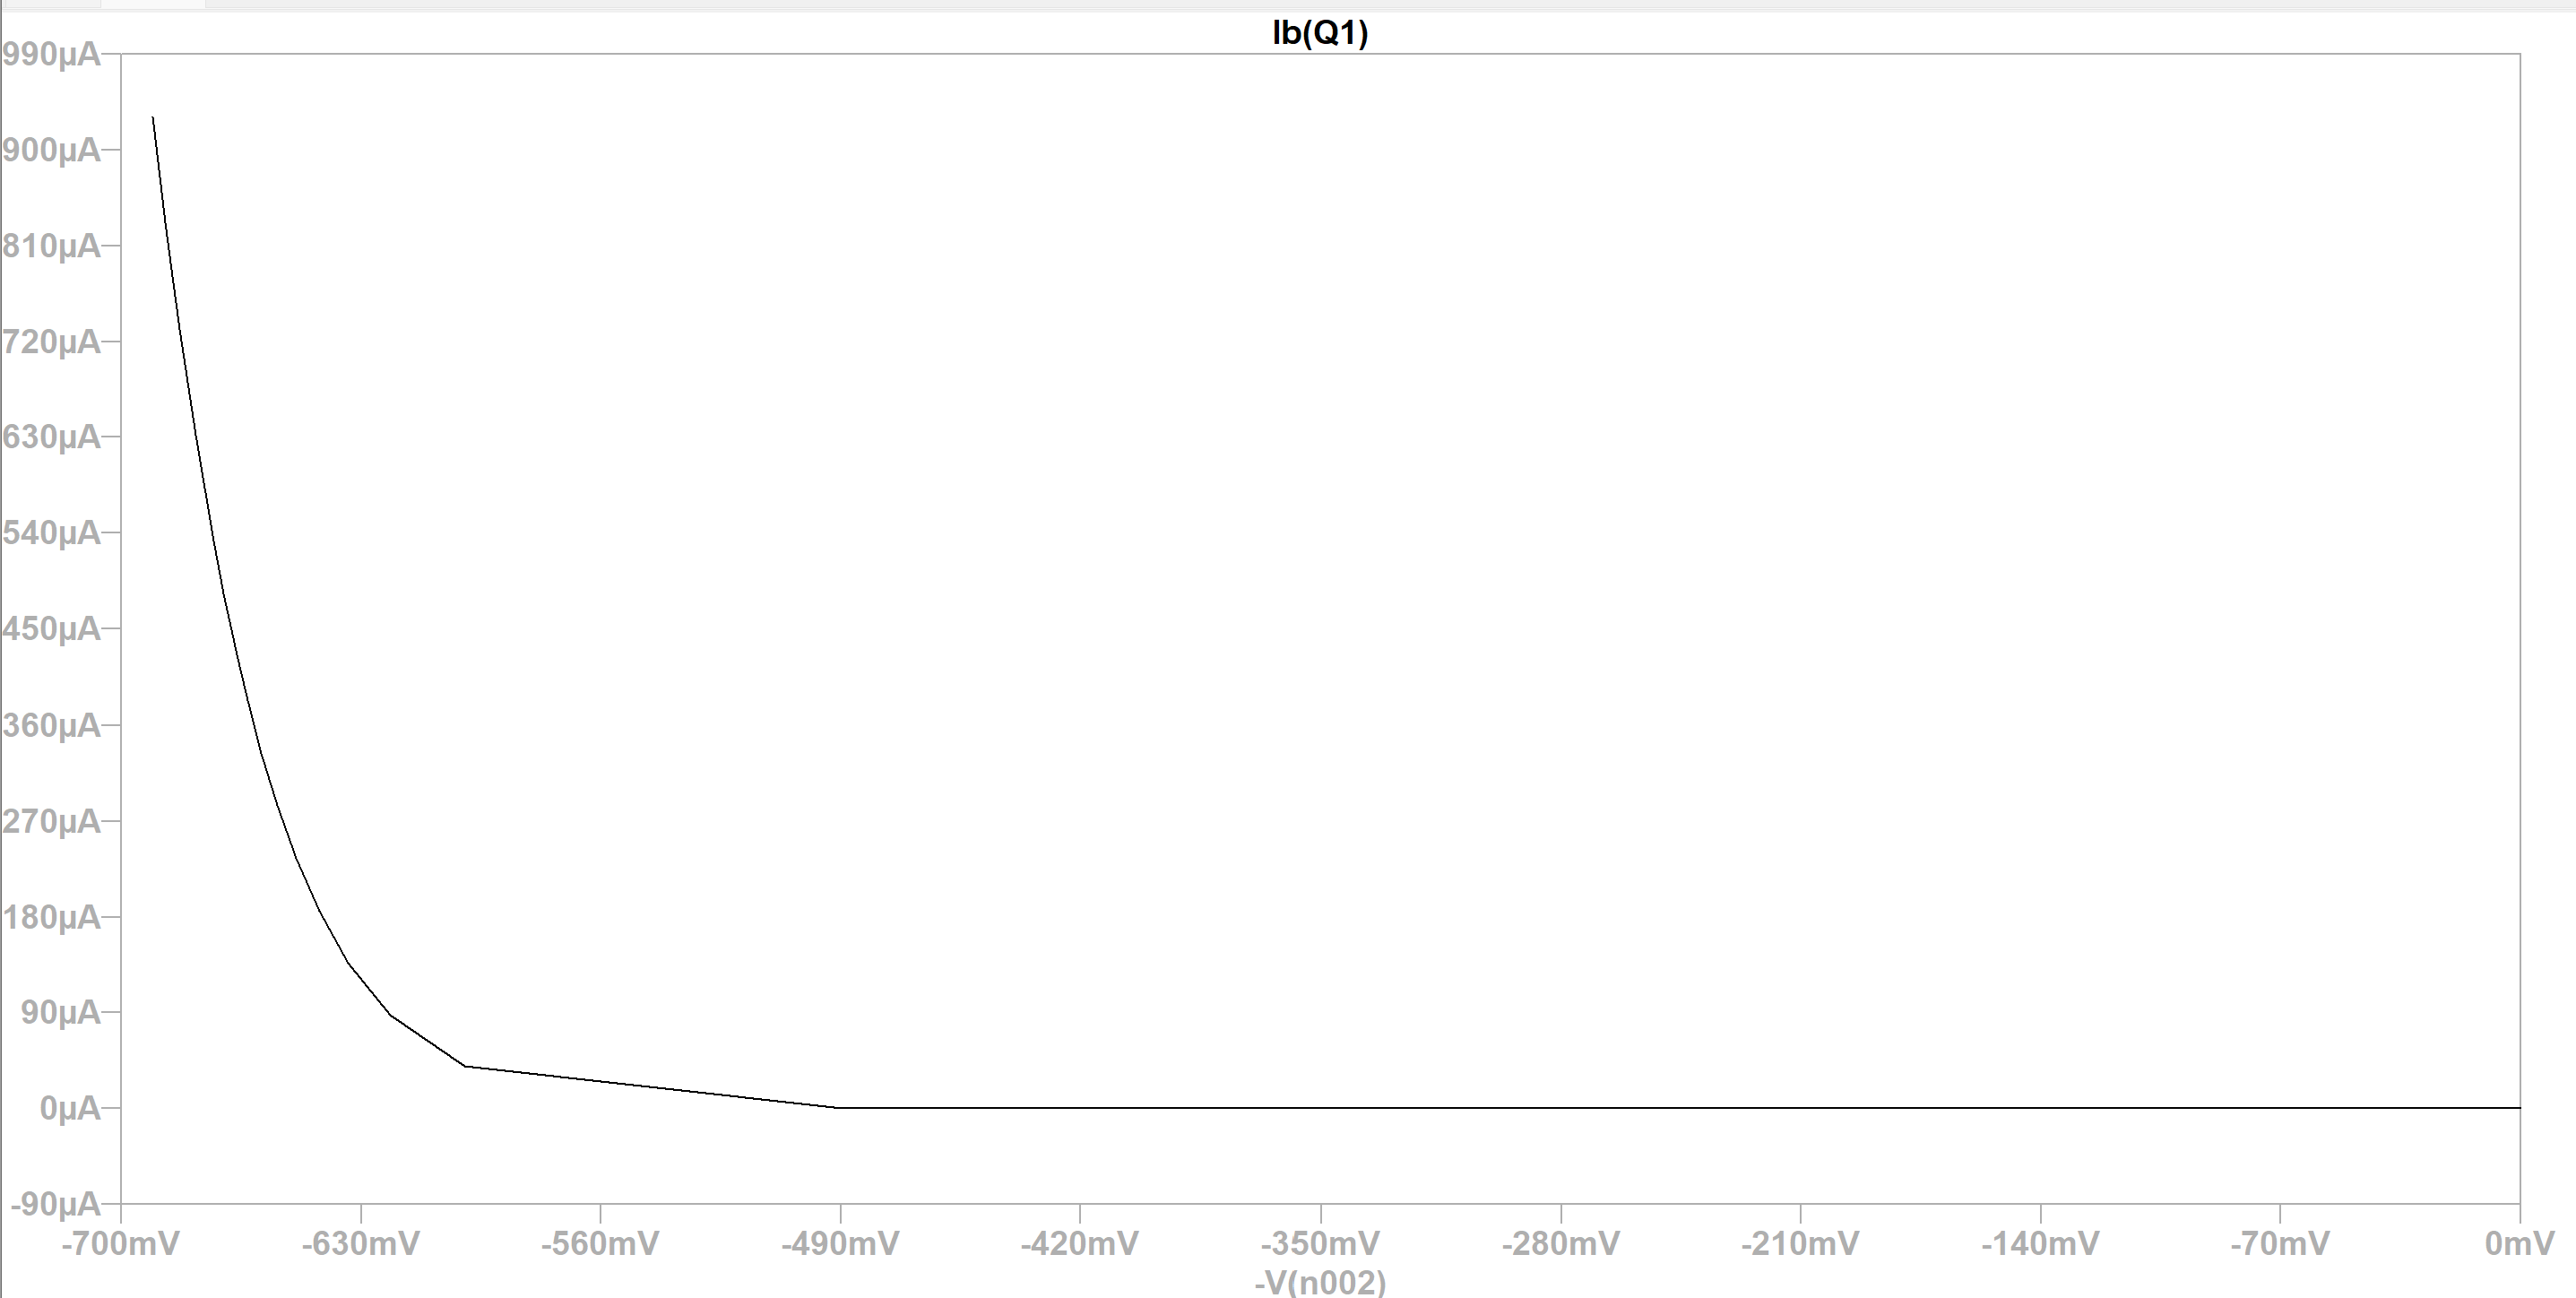
\includegraphics[width=\textwidth]{../CC-Configutation/input/input_VEC=1.png}
        \caption{$I_B$ vs $V_{BC}$ at fixed $V_{EC} = 1\text{ V}$}
    \end{subfigure}
    \hfill
    \begin{subfigure}[b]{0.45\textwidth}
        \centering
        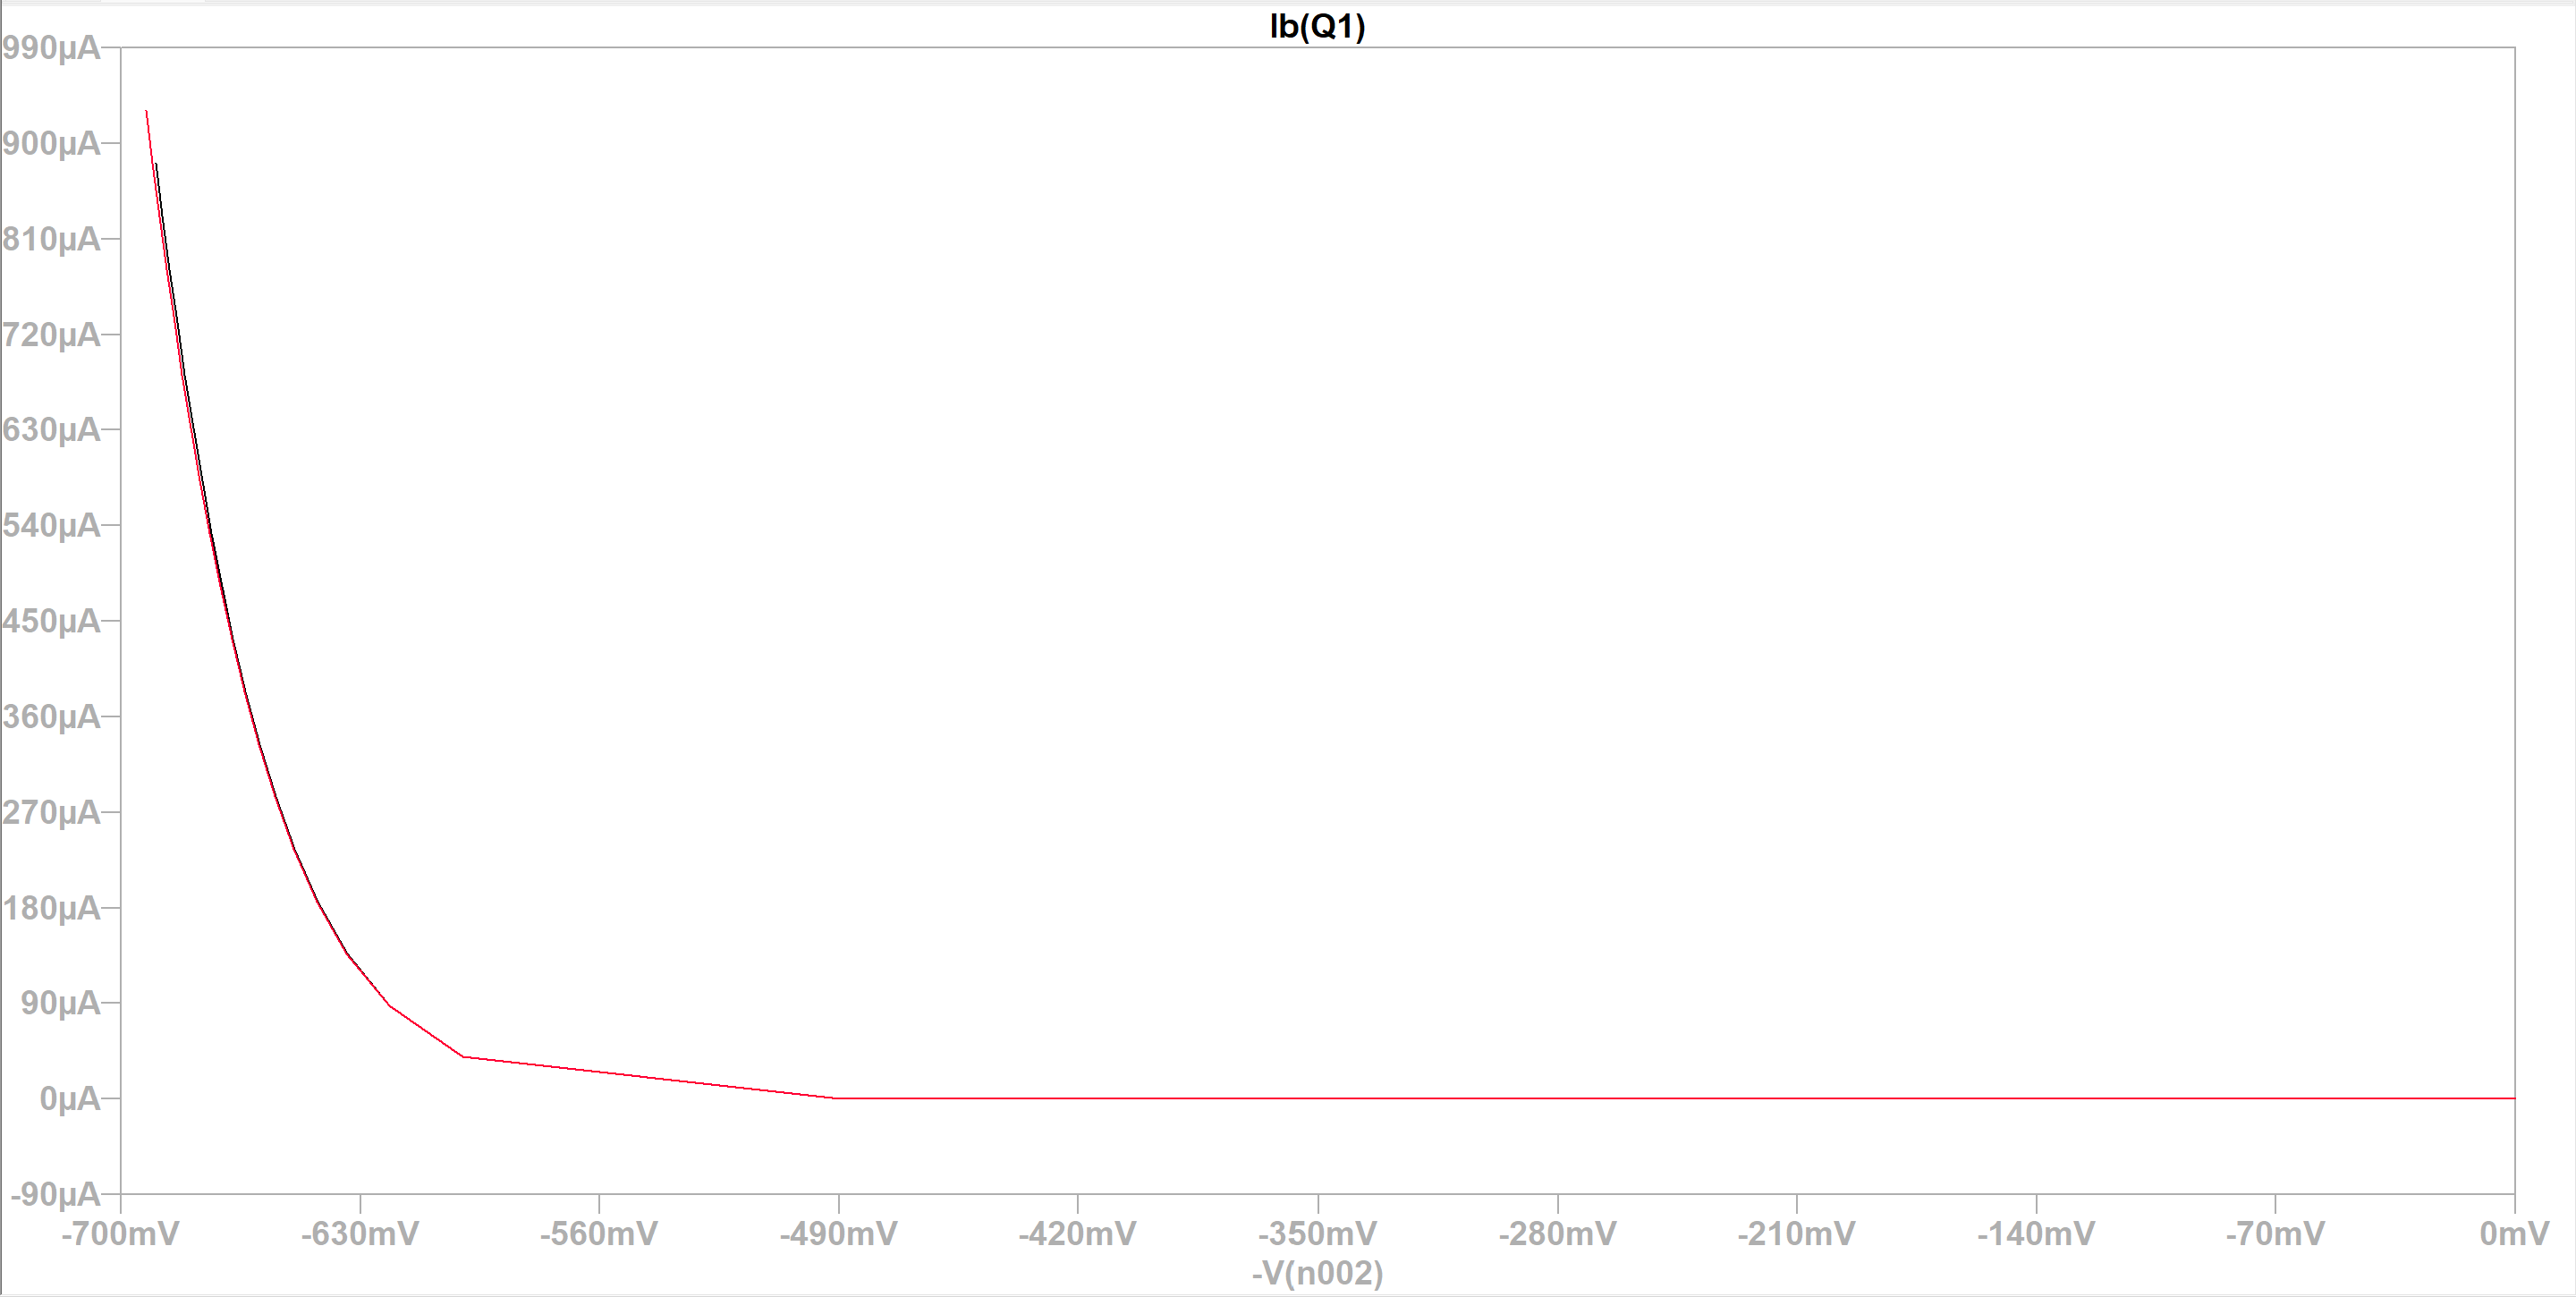
\includegraphics[width=\textwidth]{../CC-Configutation/input/input_VEC=5,10.png}
        \caption{$I_B$ vs $V_{BC}$ at fixed $V_{EC} = 5\text{ V}, 10\text{ V}$}
    \end{subfigure}
    \caption{LTspice Simulation of CC Input Characteristics ($I_B$ vs $V_{BC}$).}
    \label{fig:cc_input_sim}
\end{figure}

\subsubsection{CC Output Characteristics Simulation}
\begin{figure}[H]
    \centering
    \begin{subfigure}[b]{0.45\textwidth}
        \centering
        
\includegraphics[width=\textwidth]{../CC-Configutation/output/output_0-2.png}
        \caption{Saturation / Low Voltage Region ($V_{EC} = 0\text{--}2\text{ V}$)}
    \end{subfigure}
    \hfill
    \begin{subfigure}[b]{0.45\textwidth}
        \centering
        
\includegraphics[width=\textwidth]{../CC-Configutation/output/output_2-20.png}
        \caption{Active Region ($V_{EC} = 2\text{--}20\text{ V}$)}
    \end{subfigure}
    \caption{LTspice Simulation of CC Output Characteristics ($I_E$ vs $V_{EC}$) for $I_B = 20\ \mu\text{A}, 60\ \mu\text{A}, 100\ \mu\text{A}$.}
    \label{fig:cc_output_sim}
\end{figure}

\subsection{Experimental Observation Tables (Hardware Data)}

\begin{table}[H]
\centering
\caption{CC Input Characteristics Observation Table ($I_B$ vs $V_{BC}$)}
\begin{tabular}{c c c c c}
\toprule
\textbf{S.No.} & \textbf{$V_{BC}$ (V)} & \textbf{$I_B$ ($\mu$A) at $V_{EC}=1$V} & \textbf{$I_B$ ($\mu$A) at $V_{EC}=5$V} & \textbf{$I_B$ ($\mu$A) at $V_{EC}=10$V} \\
\midrule
1  & 0.0 & & & \\
2  & 1.0 & & & \\
3  & 2.0 & & & \\
4  & 3.0 & & & \\
5  & 4.0 & & & \\
6  & 5.0 & & & \\
7  & 6.0 & & & \\
8  & 7.0 & & & \\
9  & 8.0 & & & \\
10 & 9.0 & & & \\
11 & 10.0 & & & \\
\bottomrule
\end{tabular}
\end{table}

\begin{table}[H]
\centering
\caption{CC Output Characteristics Observation Table ($I_E$ vs $V_{EC}$)}
\begin{tabular}{c c c c c}
\toprule
\textbf{S.No.} & \textbf{$V_{EC}$ (V)} & \textbf{$I_E$ (mA) at $I_B=20\ \mu$A} & \textbf{$I_E$ (mA) at $I_B=60\ \mu$A} & \textbf{$I_E$ (mA) at $I_B=100\ \mu$A} \\
\midrule
1  & 0.0 & & & \\
2  & 0.5 & & & \\
3  & 1.0 & & & \\
4  & 1.5 & & & \\
5  & 2.0 & & & \\
6  & 4.0 & & & \\
7  & 6.0 & & & \\
8  & 8.0 & & & \\
9  & 10.0 & & & \\
10 & 15.0 & & & \\
11 & 20.0 & & & \\
\bottomrule
\end{tabular}
\end{table}

\clearpage

\section{Calculations and Verification of Relations}
\subsection{Formulae for Parameter Extraction}
\begin{enumerate}
    \item \textbf{Common Emitter Parameters:}
    \begin{equation}
        \beta = \frac{\Delta I_C}{\Delta I_B} \quad (\text{at const } V_{CE}), \quad r_{i(\text{CE})} = \frac{\Delta V_{BE}}{\Delta I_B} \quad (\text{at const } V_{CE}), \quad r_{o(\text{CE})} = \frac{\Delta V_{CE}}{\Delta I_C} \quad (\text{at const } I_B)
    \end{equation}
    \item \textbf{Common Base Parameters:}
    \begin{equation}
        \alpha = \frac{\Delta I_C}{\Delta I_E} \quad (\text{at const } V_{CB}), \quad r_{i(\text{CB})} = \frac{\Delta V_{EB}}{\Delta I_E} \quad (\text{at const } V_{CB}), \quad r_{o(\text{CB})} = \frac{\Delta V_{CB}}{\Delta I_C} \quad (\text{at const } I_E)
    \end{equation}
    \item \textbf{Common Collector Parameters:}
    \begin{equation}
        \gamma = \frac{\Delta I_E}{\Delta I_B} \quad (\text{at const } V_{EC}), \quad r_{i(\text{CC})} = \frac{\Delta V_{BC}}{\Delta I_B} \quad (\text{at const } V_{EC}), \quad r_{o(\text{CC})} = \frac{\Delta V_{EC}}{\Delta I_E} \quad (\text{at const } I_B)
    \end{equation}
\end{enumerate}

\subsection{Inter-relationship Verification}
The theoretical relations between the current gains are given by:
\begin{equation}
    \beta_{calc} = \frac{\alpha}{1 - \alpha} \quad \text{and} \quad \gamma_{calc} = \beta + 1
\end{equation}

\begin{table}[H]
\centering
\caption{Comparison of Calculated vs Directly Measured Parameters}
\begin{tabular}{l c c c}
\toprule
\textbf{Parameter / Gain} & \textbf{Directly Measured} & \textbf{Calculated from Formula} & \textbf{\% Error} \\
\midrule
Common Base Gain ($\alpha$) & & -- & -- \\
Common Emitter Gain ($\beta$) & & $\beta_{calc} = \frac{\alpha}{1-\alpha} =$ & \\
Common Collector Gain ($\gamma$) & & $\gamma_{calc} = \beta + 1 =$ & \\
\bottomrule
\end{tabular}
\end{table}

\subsection{Comparative Summary of BJT Configurations}
\begin{table}[H]
\centering
\caption{Comparison of Key Parameters across Configurations}
\begin{tabular}{l c c c}
\toprule
\textbf{Parameter} & \textbf{Common Emitter (CE)} & \textbf{Common Base (CB)} & \textbf{Common Collector (CC)} \\
\midrule
\textbf{Input Resistance ($r_i$)} & Medium ($\approx 1\text{ k}\Omega$) & Low ($\approx 20\ \Omega$) & High ($\approx 300\text{ k}\Omega$) \\
\textbf{Output Resistance ($r_o$)} & Medium ($\approx 50\text{ k}\Omega$) & Very High ($\approx 1\text{ M}\Omega$) & Low ($\approx 50\ \Omega$) \\
\textbf{Current Gain} & High ($\beta \approx 100$) & Low ($\alpha < 1$) & High ($\gamma \approx 101$) \\
\textbf{Voltage Gain} & High & High & $\approx 1$ (Unity) \\
\textbf{Phase Shift} & $180^\circ$ & $0^\circ$ & $0^\circ$ \\
\textbf{Primary Application} & Audio / General Amplification & High Frequency Amplification & Impedance Matching / Buffer \\
\bottomrule
\end{tabular}
\end{table}

\section{Results and Conclusion}
\begin{enumerate}
    \item The input and output characteristics of the BC547 NPN transistor were simulated in LTspice and studied for Common Emitter (CE), Common Base (CB), and Common Collector (CC) configurations.
    \item The schematics and simulation waveforms for each case were integrated and analyzed.
    \item The observation tables are prepared for logging experimental hardware readings. Upon completing physical lab testing, calculated parameters ($r_i, r_o, \alpha, \beta, \gamma$) will be evaluated to verify the theoretical relationships $\beta = \frac{\alpha}{1-\alpha}$ and $\gamma = \beta + 1$.
\end{enumerate}

\end{document}
